\setcounter{chapter}{6}
\chapter{Phase 1 FPix upgrade module production}\label{ch:pixel}

\section{Introduction}

In chapter \ref{ch:cms}, a description of the CMS pixel detector used during the collection of the data sets, considered in this analysis, was presented. During the extended year-end technical stop (EYETS) 2017, the complete CMS pixel detector was replaced in order to support the full performance of the CMS experiment under the higher radiation conditions produced by the increasing instantaneous luminosity delivered  by the LHC accelerator. It also was designed to address and mitigate the identified weaknesses in the previous system.

In this chapter, a description of the upgraded detector will be presented. Emphasis will be put on the contributions made by the University of Nebraska - Lincoln (UNL) HEP group. The contribution consisted of the assembly of about 600 of the modules that make up the phase 1 upgraded forward pixel detector (FPix); in particular, the gluing and encapsulation stages will be described in detail since they are my contributions. A complete description of the upgrade design and plans is presented in Reference \cite{pix_tdr} which is the main source of the information contained in this section unless additional references are provided.   

\section{CMS pixel detector upgrade}

The previous pixel detector was designed to record efficiently and with high precision the first three space-points near the interaction region, in the range of $|\eta|<2.5$,  at an instantaneous luminosity of $1\times10^{34}$ cm$^{-2}$s$^{-1}$ and a bunch crossing each 25 ns. An average pileup of about 25 simultaneous overlapping events is expected. The increasing luminosity would affect the performance of the detector reducing track reconstruction efficiency, and increasing the data losses caused by the degradation of the readout system; furthermore, if the LHC runs with 50 ns bunch spacing at twice the luminosity, then the data losses would increase almost exponentially, to losses of 50\% for the innermost layer. An illustration of the foreseen reduced performance in tracking efficiency and data loss is shown in Figure \ref{fig:reduced_performance} in the case of simulated \ttbar events at instantaneous luminosity up to $2\times10^{34}$ cm$^{-2}$s$^{-1}$ with 25 ns and 50 ns bunch spacing. The increasing fake rate is also shown. In conclusion, the previous pixel detector was not able to perform efficiently under the new luminosity, pileup, radiation, and running conditions.  

\begin{figure}[!h]
\centering
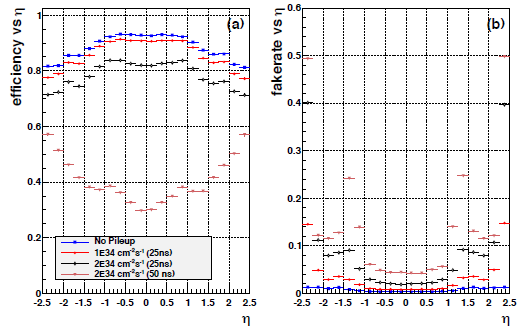
\includegraphics[width=0.9\textwidth]{pixel/reducedperformance2}
%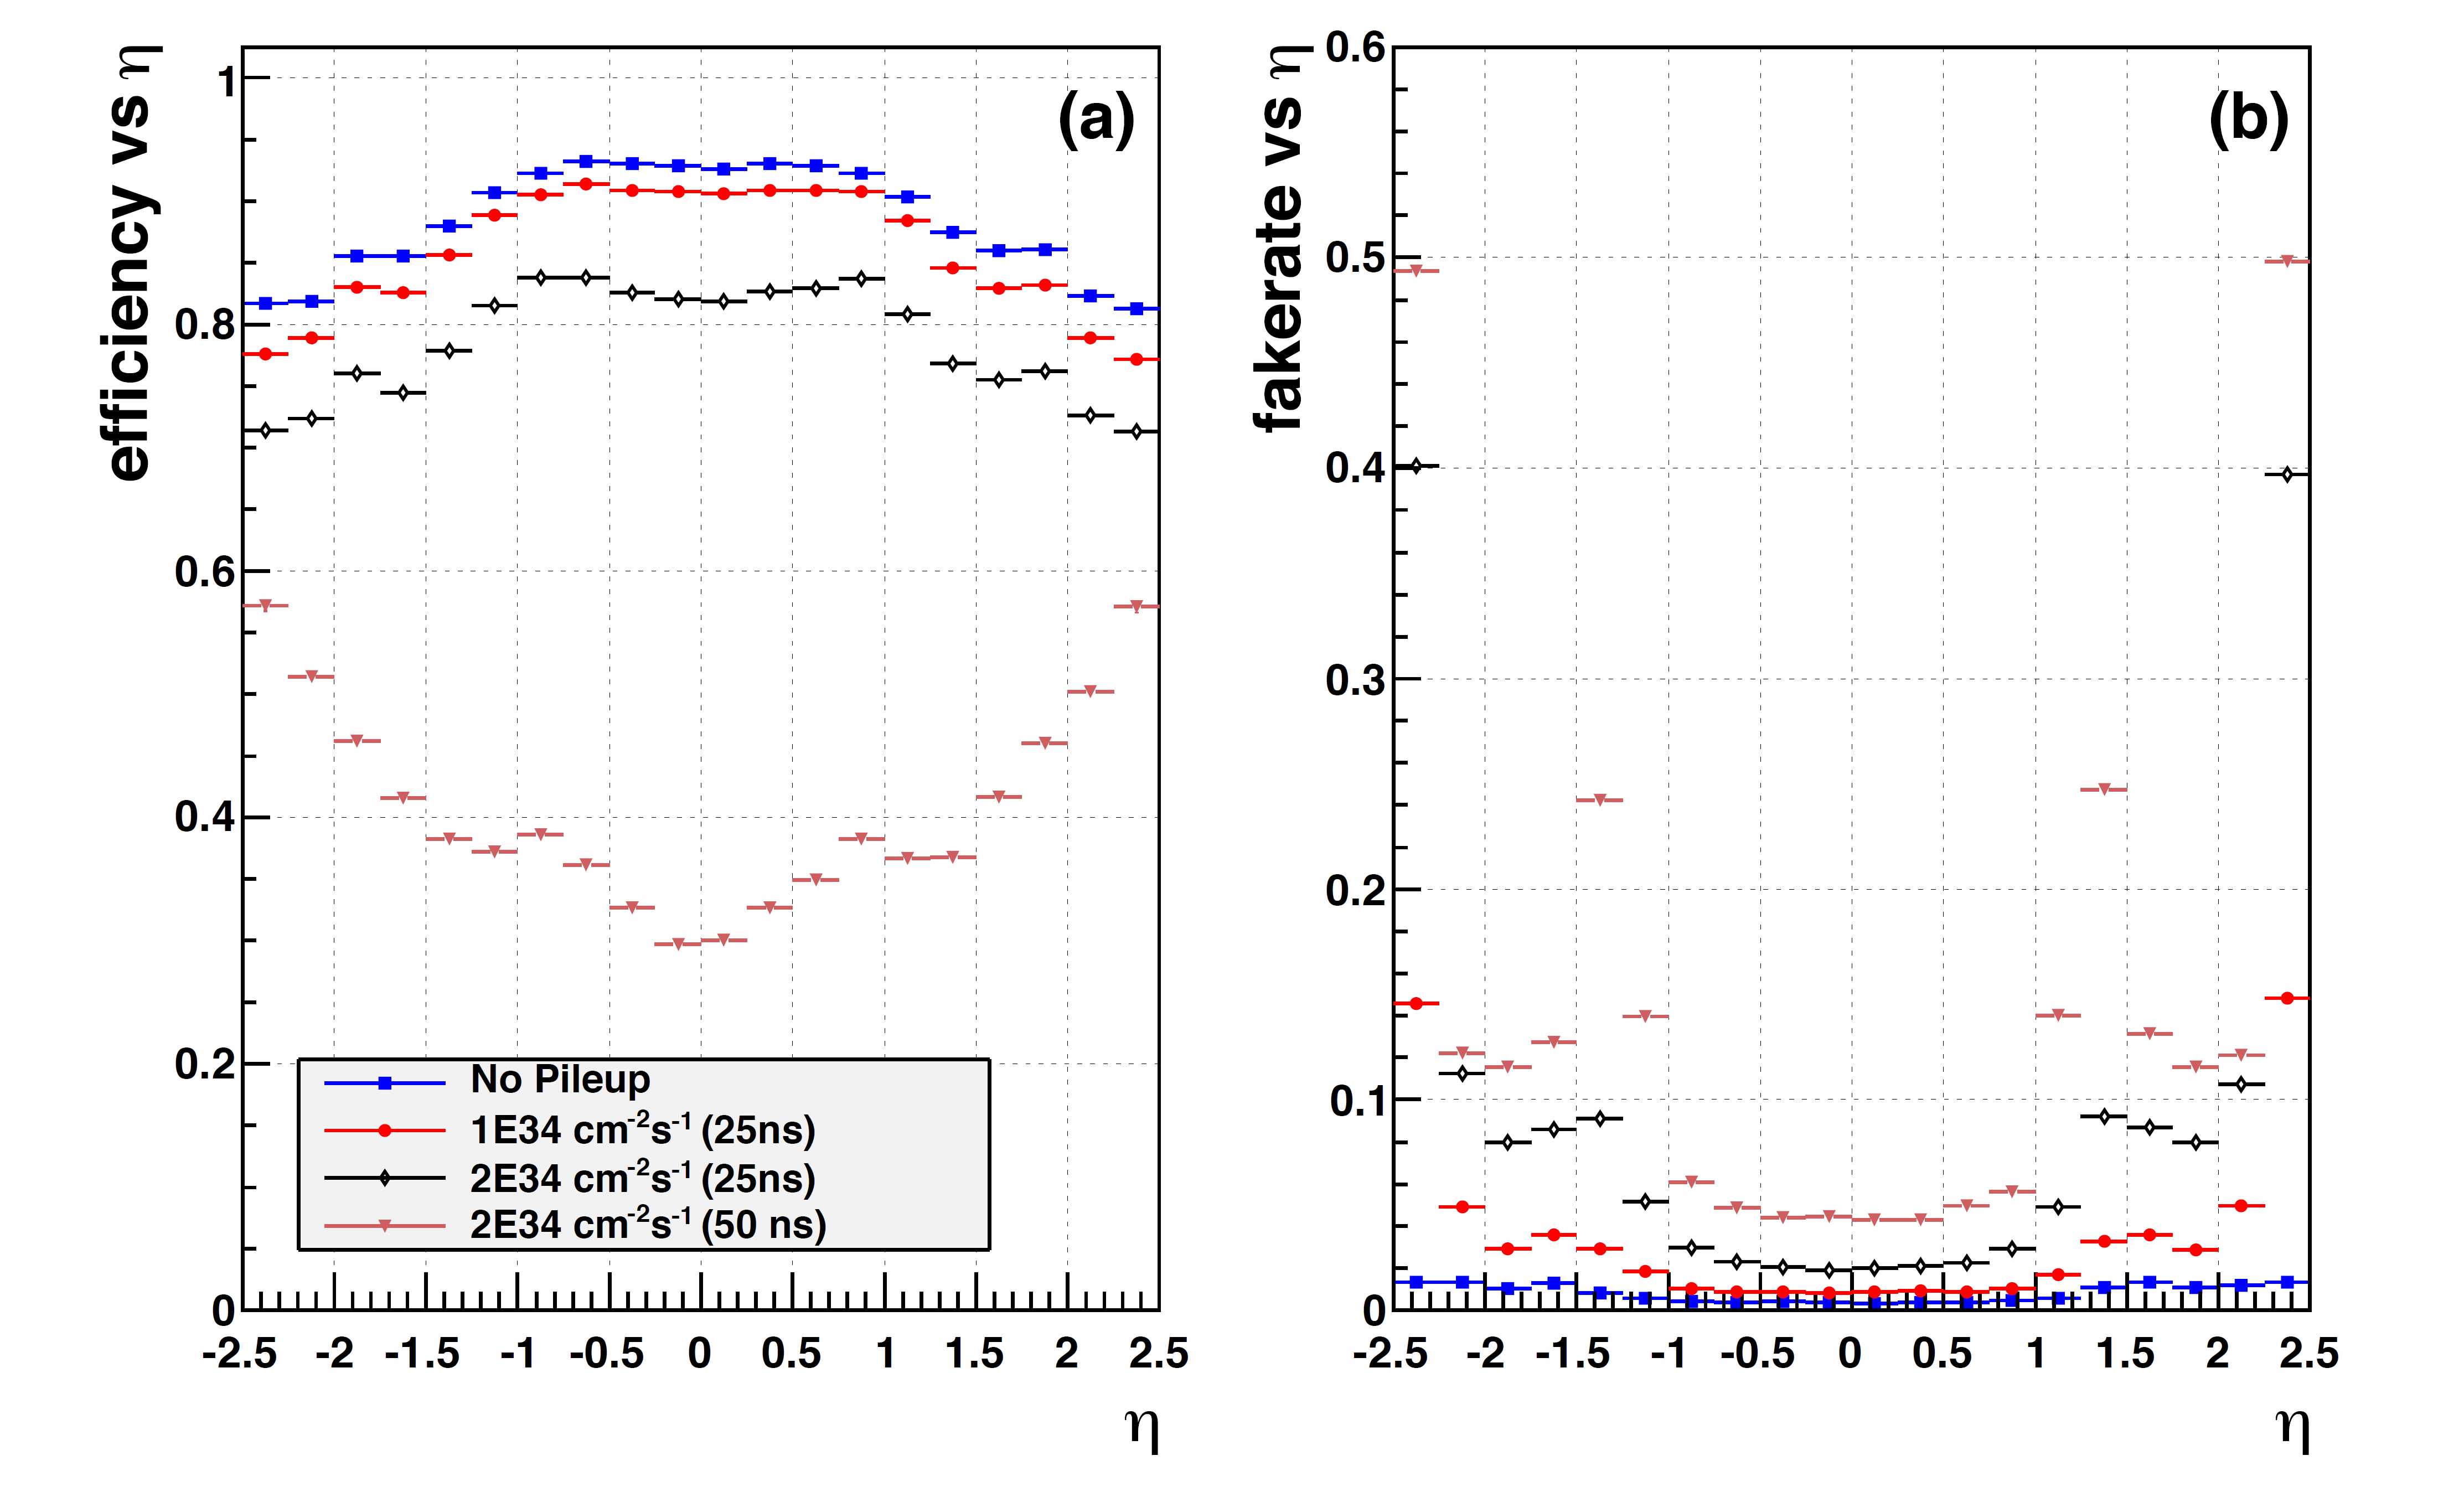
\includegraphics[width=0.9\textwidth]{pixel/reducedperformance}
\caption[Expected performance of the previous pixel detector in simulated \ttbar events.]{Expected performance of the previous pixel detector in simulated \ttbar events: a) efficiency; b) fake rate. Conventions are the same for both plots, considering zero pileup (blue squares), average pileup of 25 (red dots), average pileup of 50 (black diamonds), and average pileup of 100 (magenta triangles).}\label{fig:reduced_performance}
\end{figure}

The current system is designed to offer high performance under these new operational conditions; it is composed of four-layers/three-disks, low mass silicon pixel detectors providing a high performance tracking in the high luminosity environment.

%% The design was led by the following requirements\footnote{Taken literally from the technical design report.} 

%% \bit
%% \item In running with 50 or more pile-up, maintain the high efficiencies and low fake rates.
%% \item New pixel readout chip (ROC) to minimize data loss due to latencies and limited buffering in high luminosity running.
%% \item Minimize degradation due to radiation damage.
%% \item Optimized detector layout for 4-pixel-hit coverage over the \etac range with minimal innermost layer radius improving pattern recognition and track reconstruction.
%% \item To reduce material, adopt two-phase $CO_2$ cooling and light-weight mechanical support, moving the electronic boards and connections out of the tracking volume.
%% \item To reuse the current patch panel and off-detector services, cooling pipes, cables, and fibers, adopt DC-DC power converters and higher bandwidth electronics.
%% \item Reduce number of module types and interfaces simplifying production and maintenance.
%% \item New smaller diameter beam pipe to accommodate the placement of the inner pixel layer closer to the interaction region.
%% \eit

The upgraded detector is expected to provide higher efficiencies, lower fake rates, lower dead-time/data-loss, and an extended lifetime of the detector, which translate in better muon ID, b-tagging, photon/electron ID, and tau reconstruction, at both HLT and offline levels. No details about the performance of the current pixel detector are given here since that matter falls beyond the purpose of this document; however, it is documented in Reference\cite{pixel_performance}.

Figure \ref{fig:new_pix} shows the layout of the upgraded pixel detector. The old 3-layer barrel (BPIX), 2-disk endcap (FPIX) system is replaced with a 4-layer barrel, 3-disk endcap system. The additional barrel layer and forward disk provide redundancy for the track pattern recognition and reconstruction.

\begin{figure}[!h]
\centering
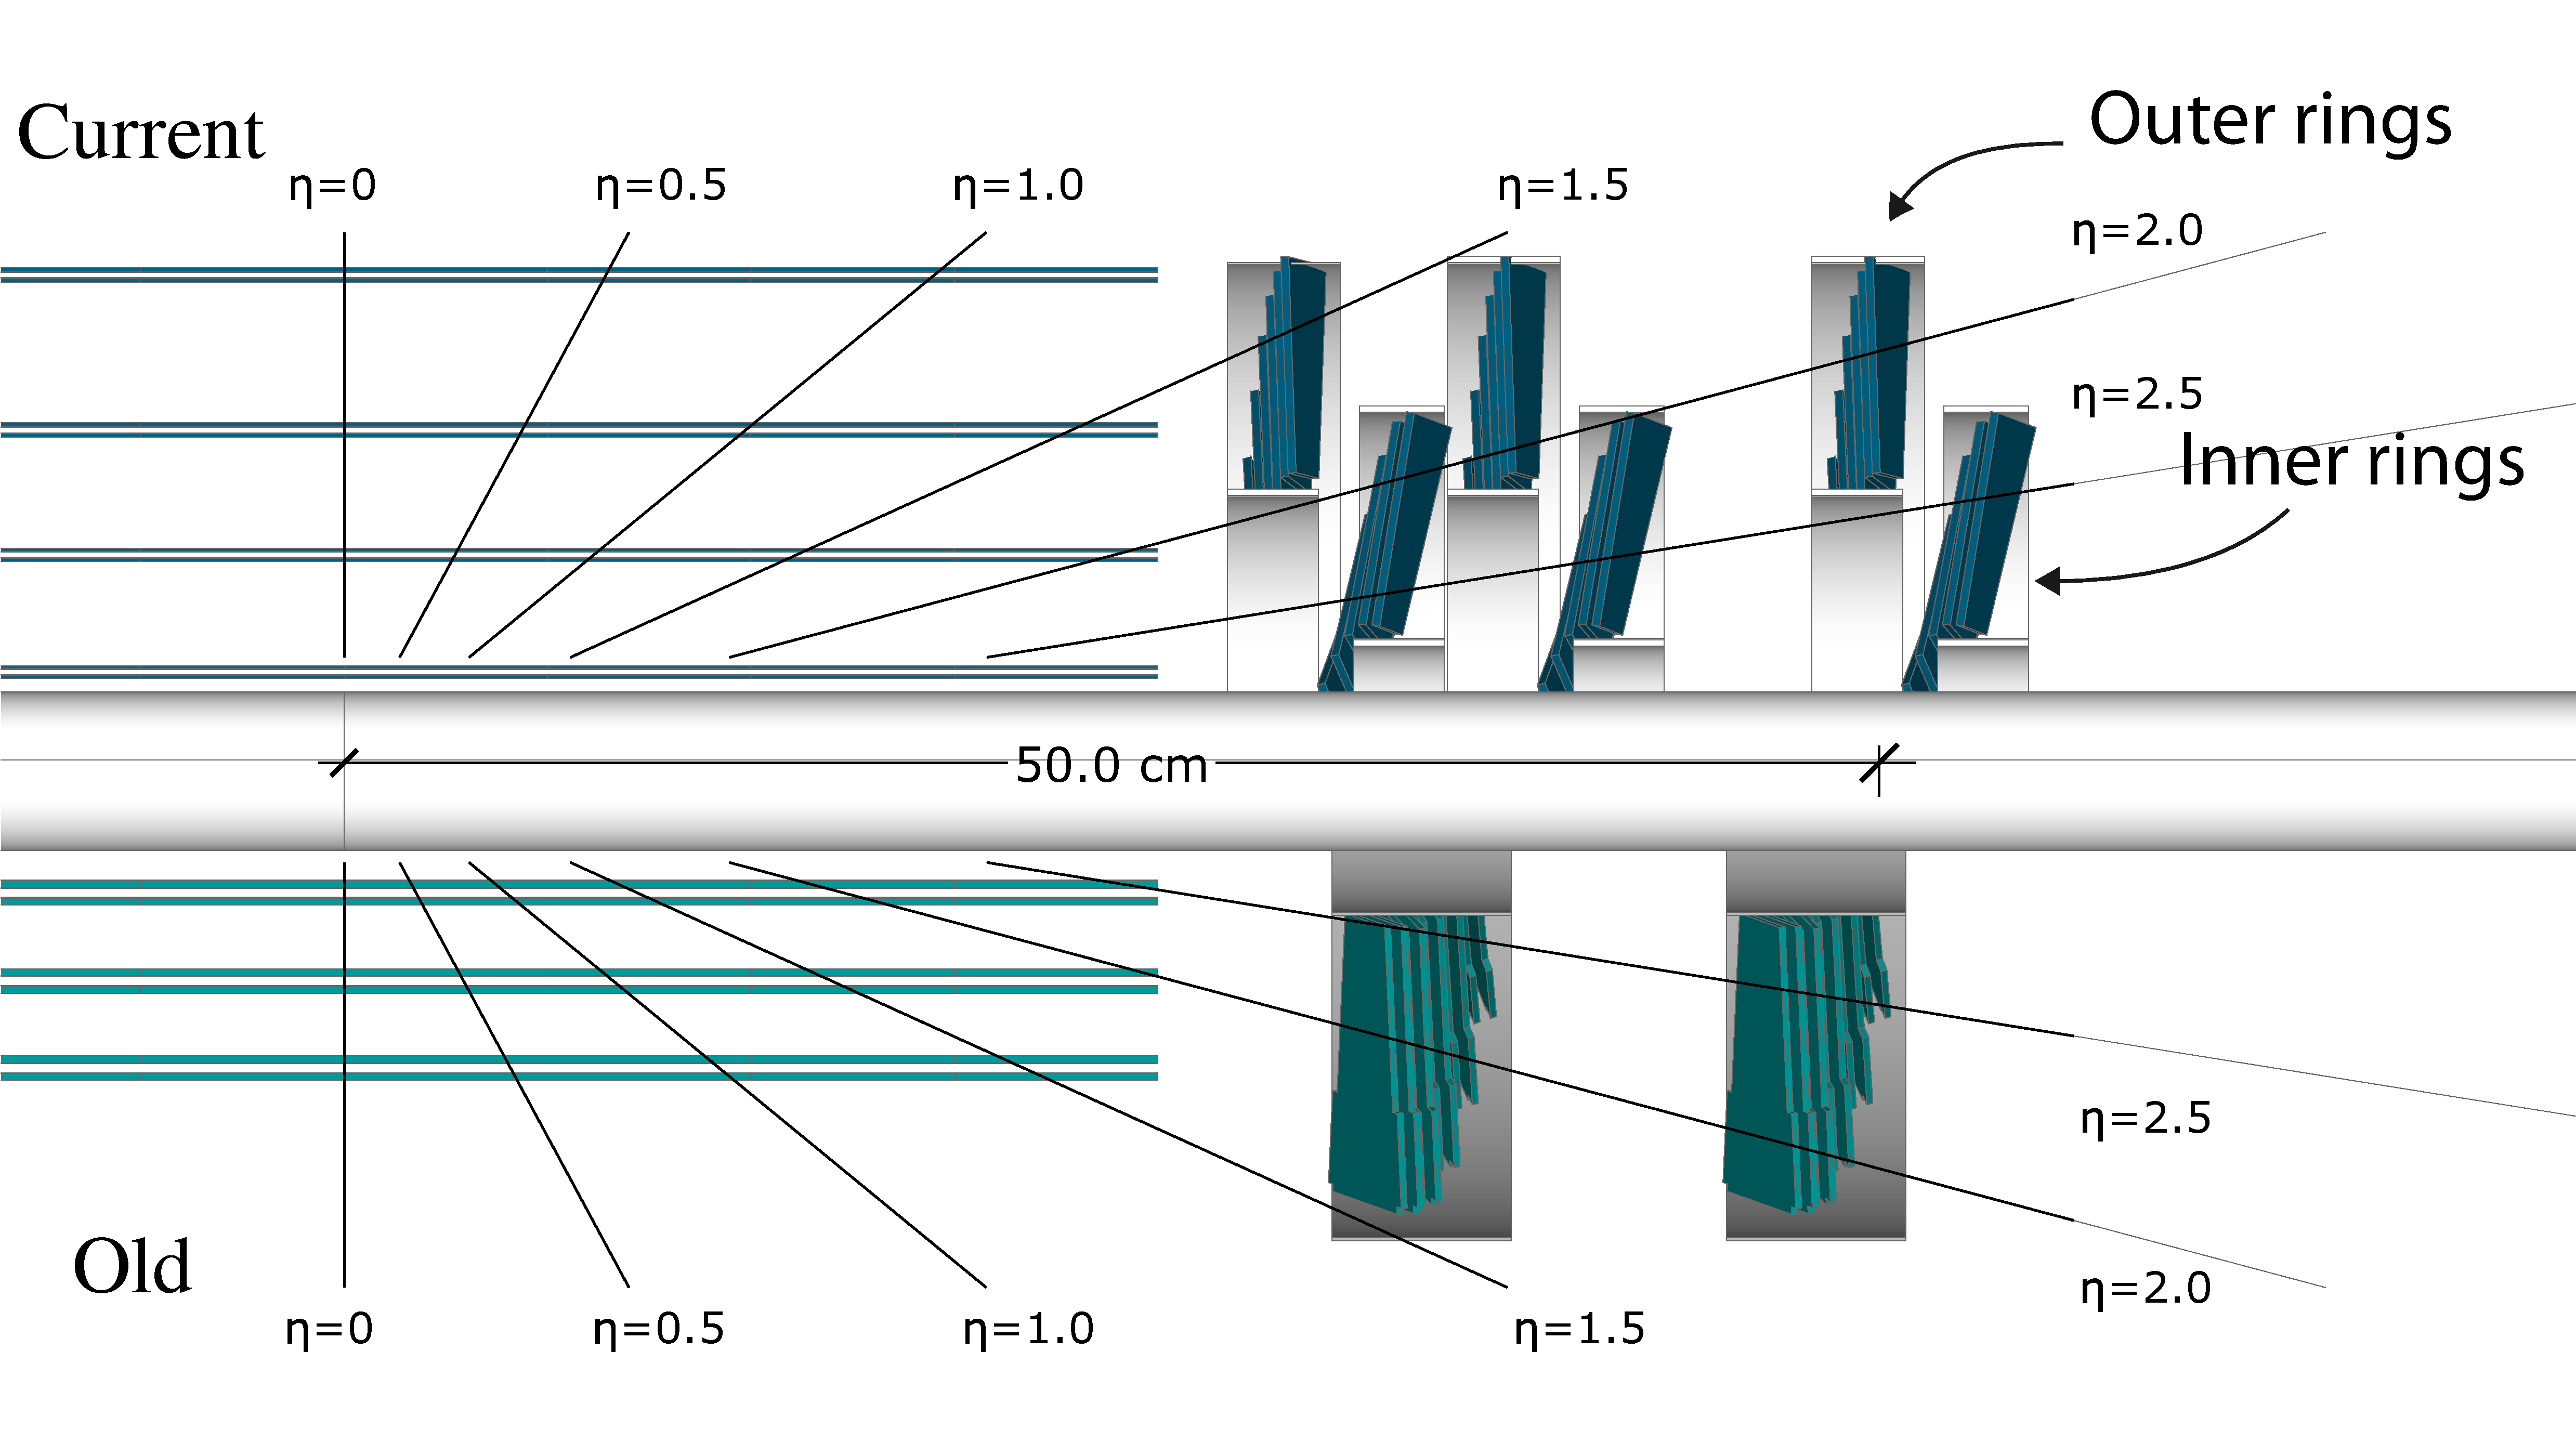
\includegraphics[width=0.6\textwidth]{fpix1.pdf}
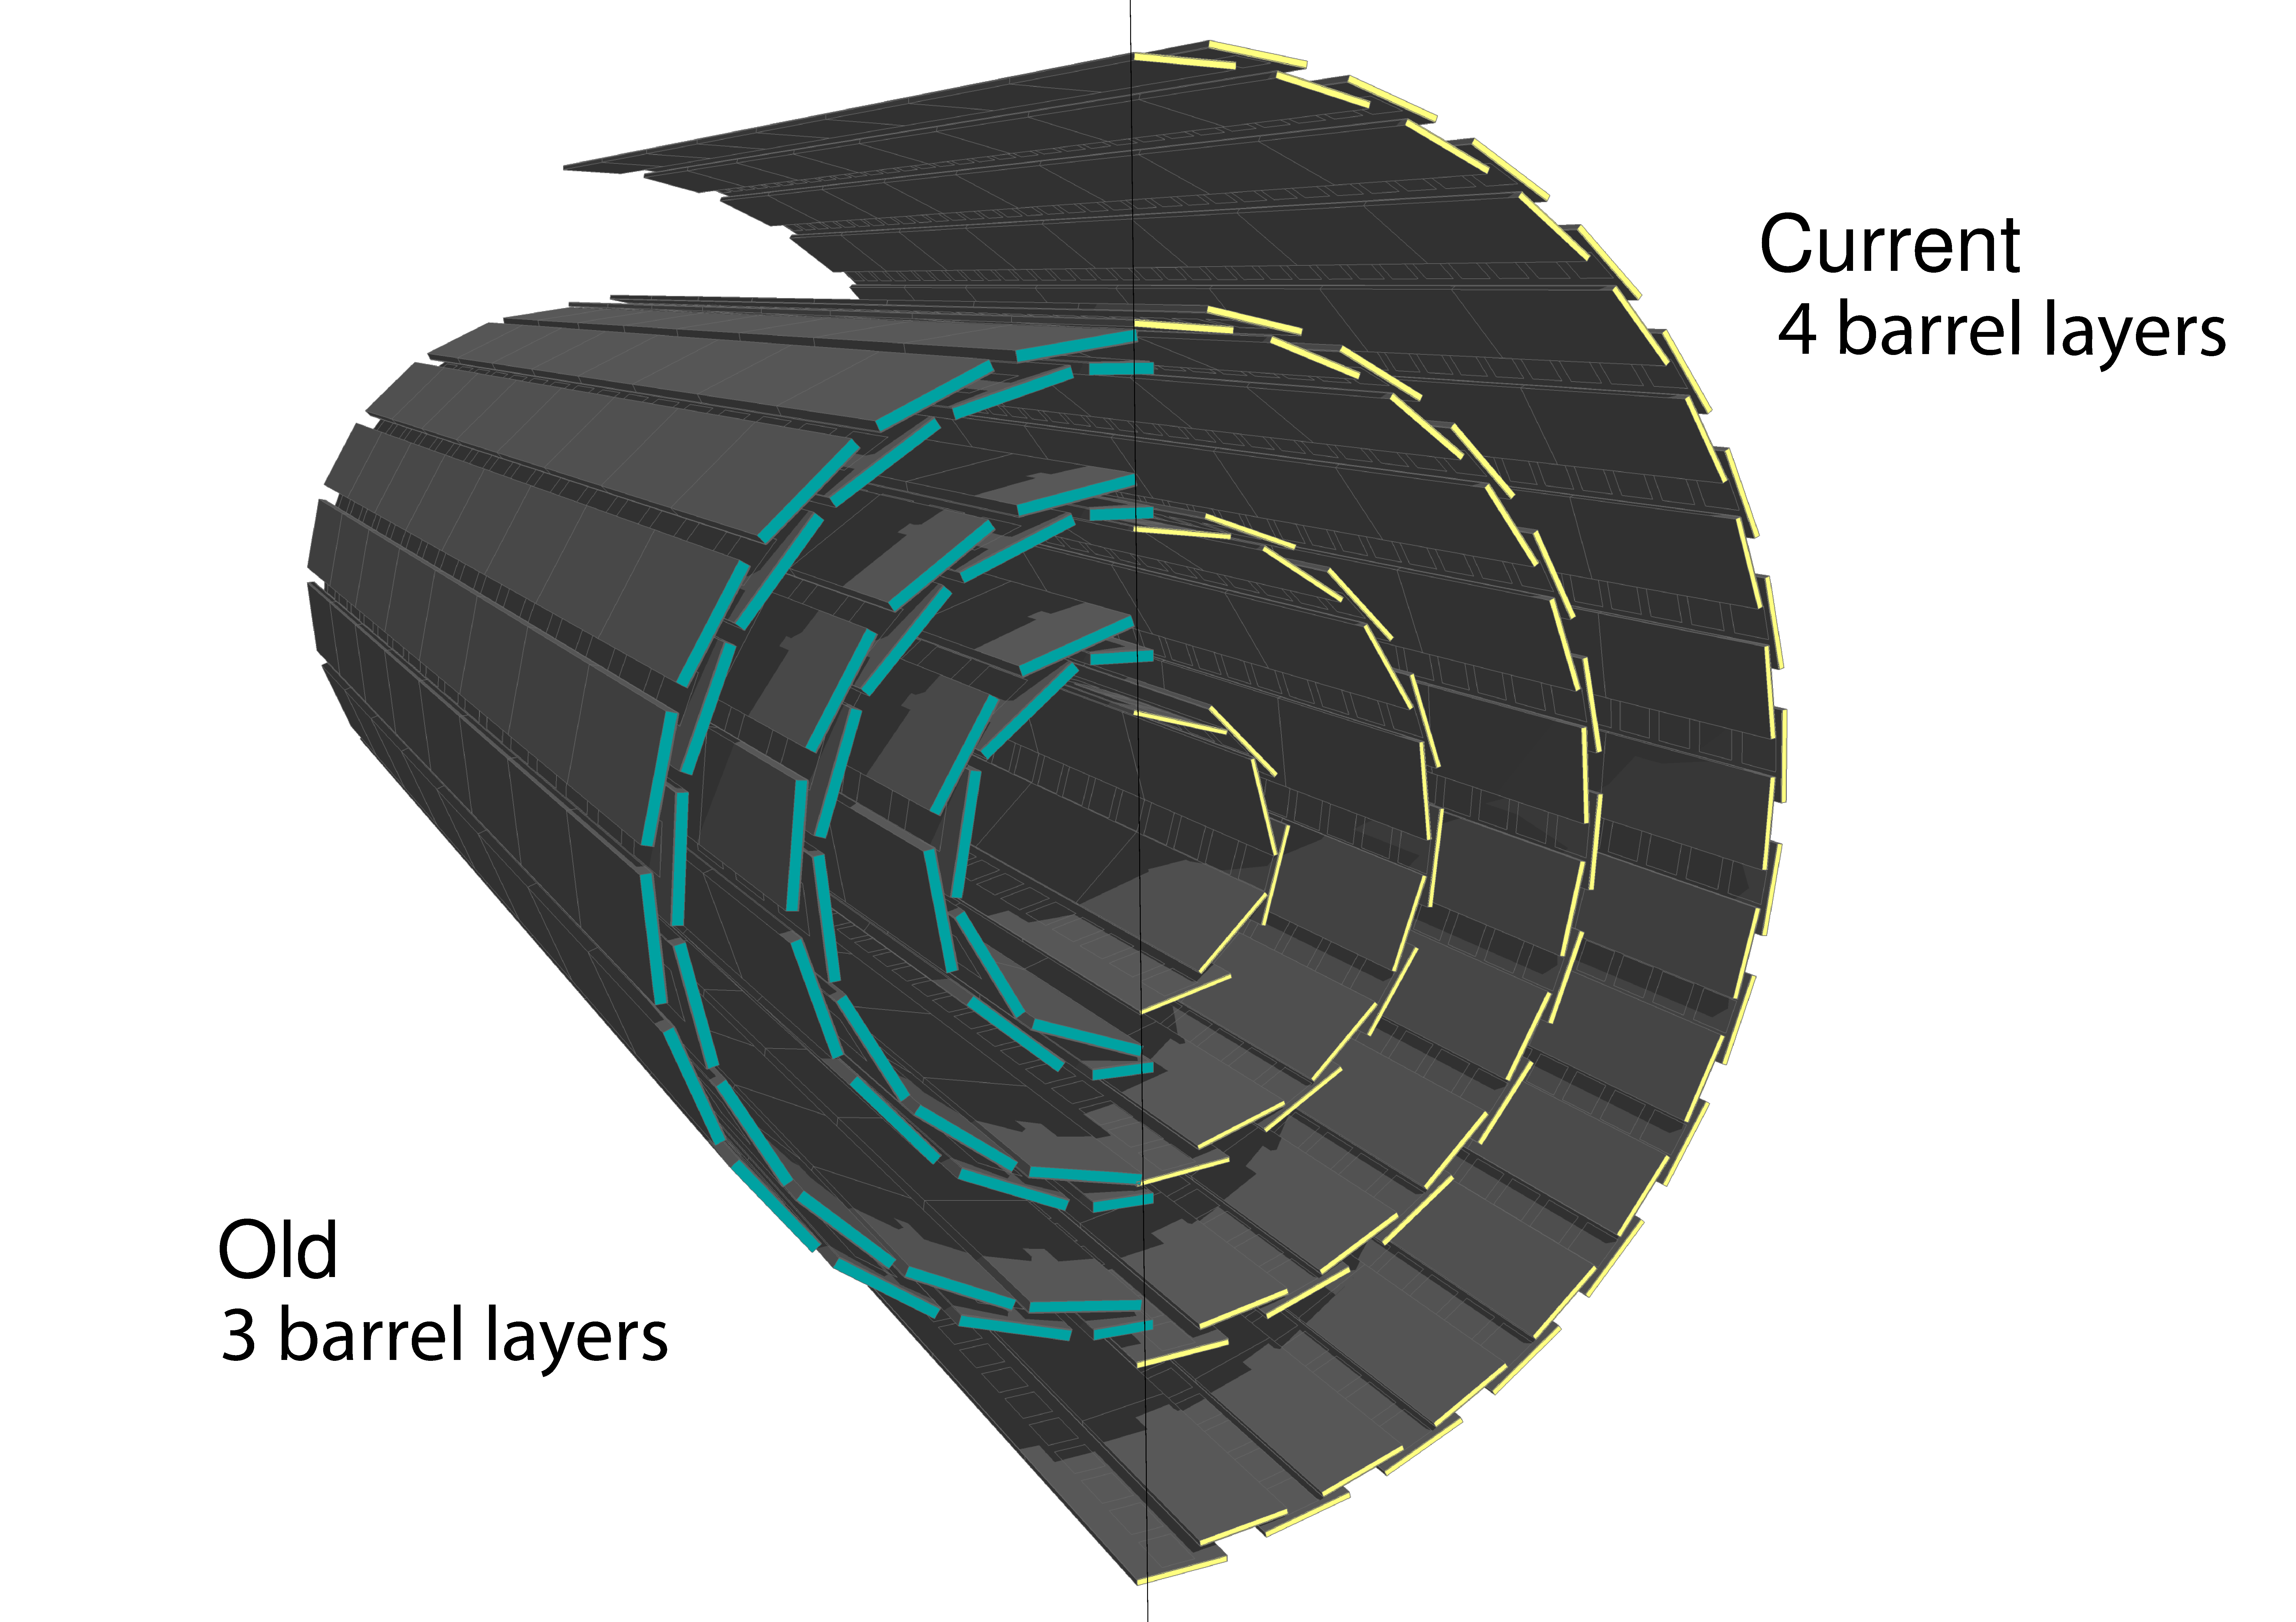
\includegraphics[width=0.39\textwidth]{bpix1.pdf}
\caption[Layout of the upgraded and old pixel detectors.]{Layout and comparison of the layers and disks in the current and old pixel detectors.}\label{fig:new_pix}
\end{figure}

\section{Phase 1 FPix upgrade}

The Phase 1 upgraded FPix system is composed of three disks in each endcap, located at each end of the barrel detector, with a radial coverage ranging from 4.5 to 16.1 cm. The first disk is located along the beam line at 29.1 cm from the IP; the second and third disks are located at 39.6 cm and 51.6 cm from the IP; each disk consists of two half disks. Some of the main features of the upgraded FPix System are:
\bit
\item Pixel size: $100 \times 150$ $\mu$m 
\item Only one type of modules: 2x8 ROC modules
\item Modules oriented radially to improve resolution in $r-\phi$.
\item Minimize the gap in 4-hit coverage between the end of the 4th-barrel layer and the forward-most disk.
\item All three identical disks on each side of the IP.
\eit

Figure \ref{fig:fpix_layout} shows a schematic structure of the FPix half disk; each half disk is composed of two sections, inner and outer, where the pixel modules are assembled.

\begin{figure}[!h]
  \centering
  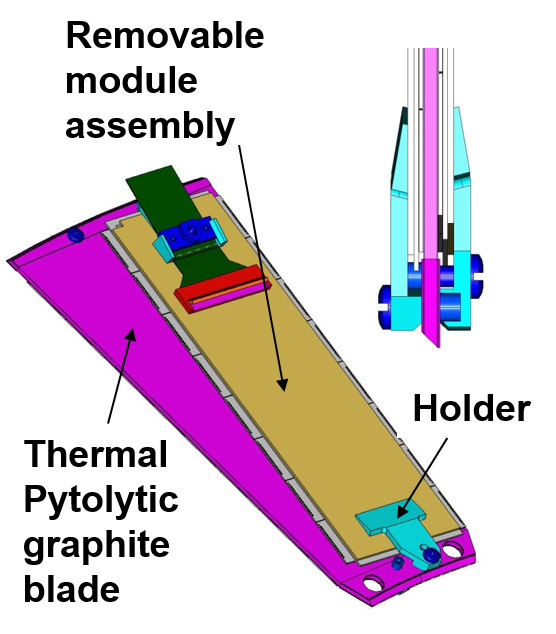
\includegraphics[width=0.32\textwidth]{pixel/module1}
  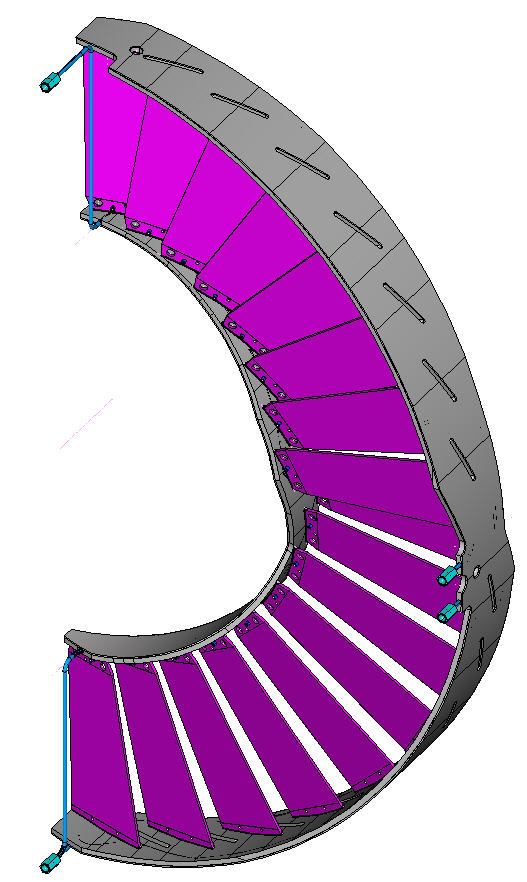
\includegraphics[width=0.32\textwidth]{pixel/half_disk_inner}
  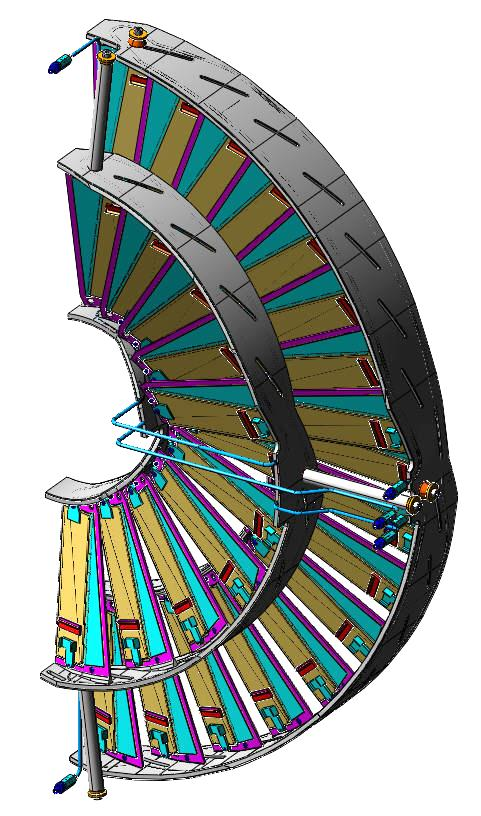
\includegraphics[width=0.32\textwidth]{pixel/half_disk}
\caption[FPix half disk design.]{FPix half disk design; FPix module (left) mounted on a blade, outer half disk (center), assembled half disk (right).}\label{fig:fpix_layout}
\end{figure}

In total, there are 56 modules (896 ROCs) per half-disk, 34 modules in the outer ring and 22 modules in the inner ring. The pixel modules are attached to the blades by a pair of module holders. Modules are designed to be removable and replaceable without disassembling the half-disks; thus those modules that suffer failure or degradation can be easily replaced during an annual technical stop.

Blades on the outer assembly are rotated by 20$^o$ forming a turbine-like geometry; in addition, they are arranged in an inverted cone array with the blades tilted by 12$^o$ with respect to the IP in order to guarantee excellent resolution in both the azimuthal and radial directions throughout the FPIX acceptance angle for the inner assembly.

\section{FPix module structure}

\begin{figure}[!h]
  \centering
  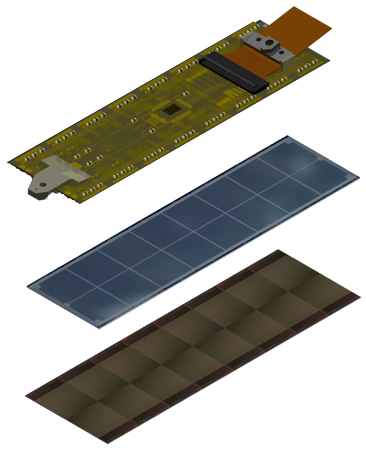
\includegraphics[width=0.33\textwidth]{pixel/fpix_structure1}
  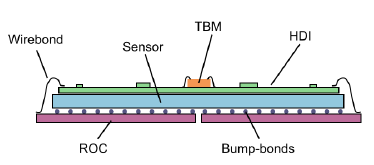
\includegraphics[width=0.63\textwidth]{pixel/fpix_structure2}
  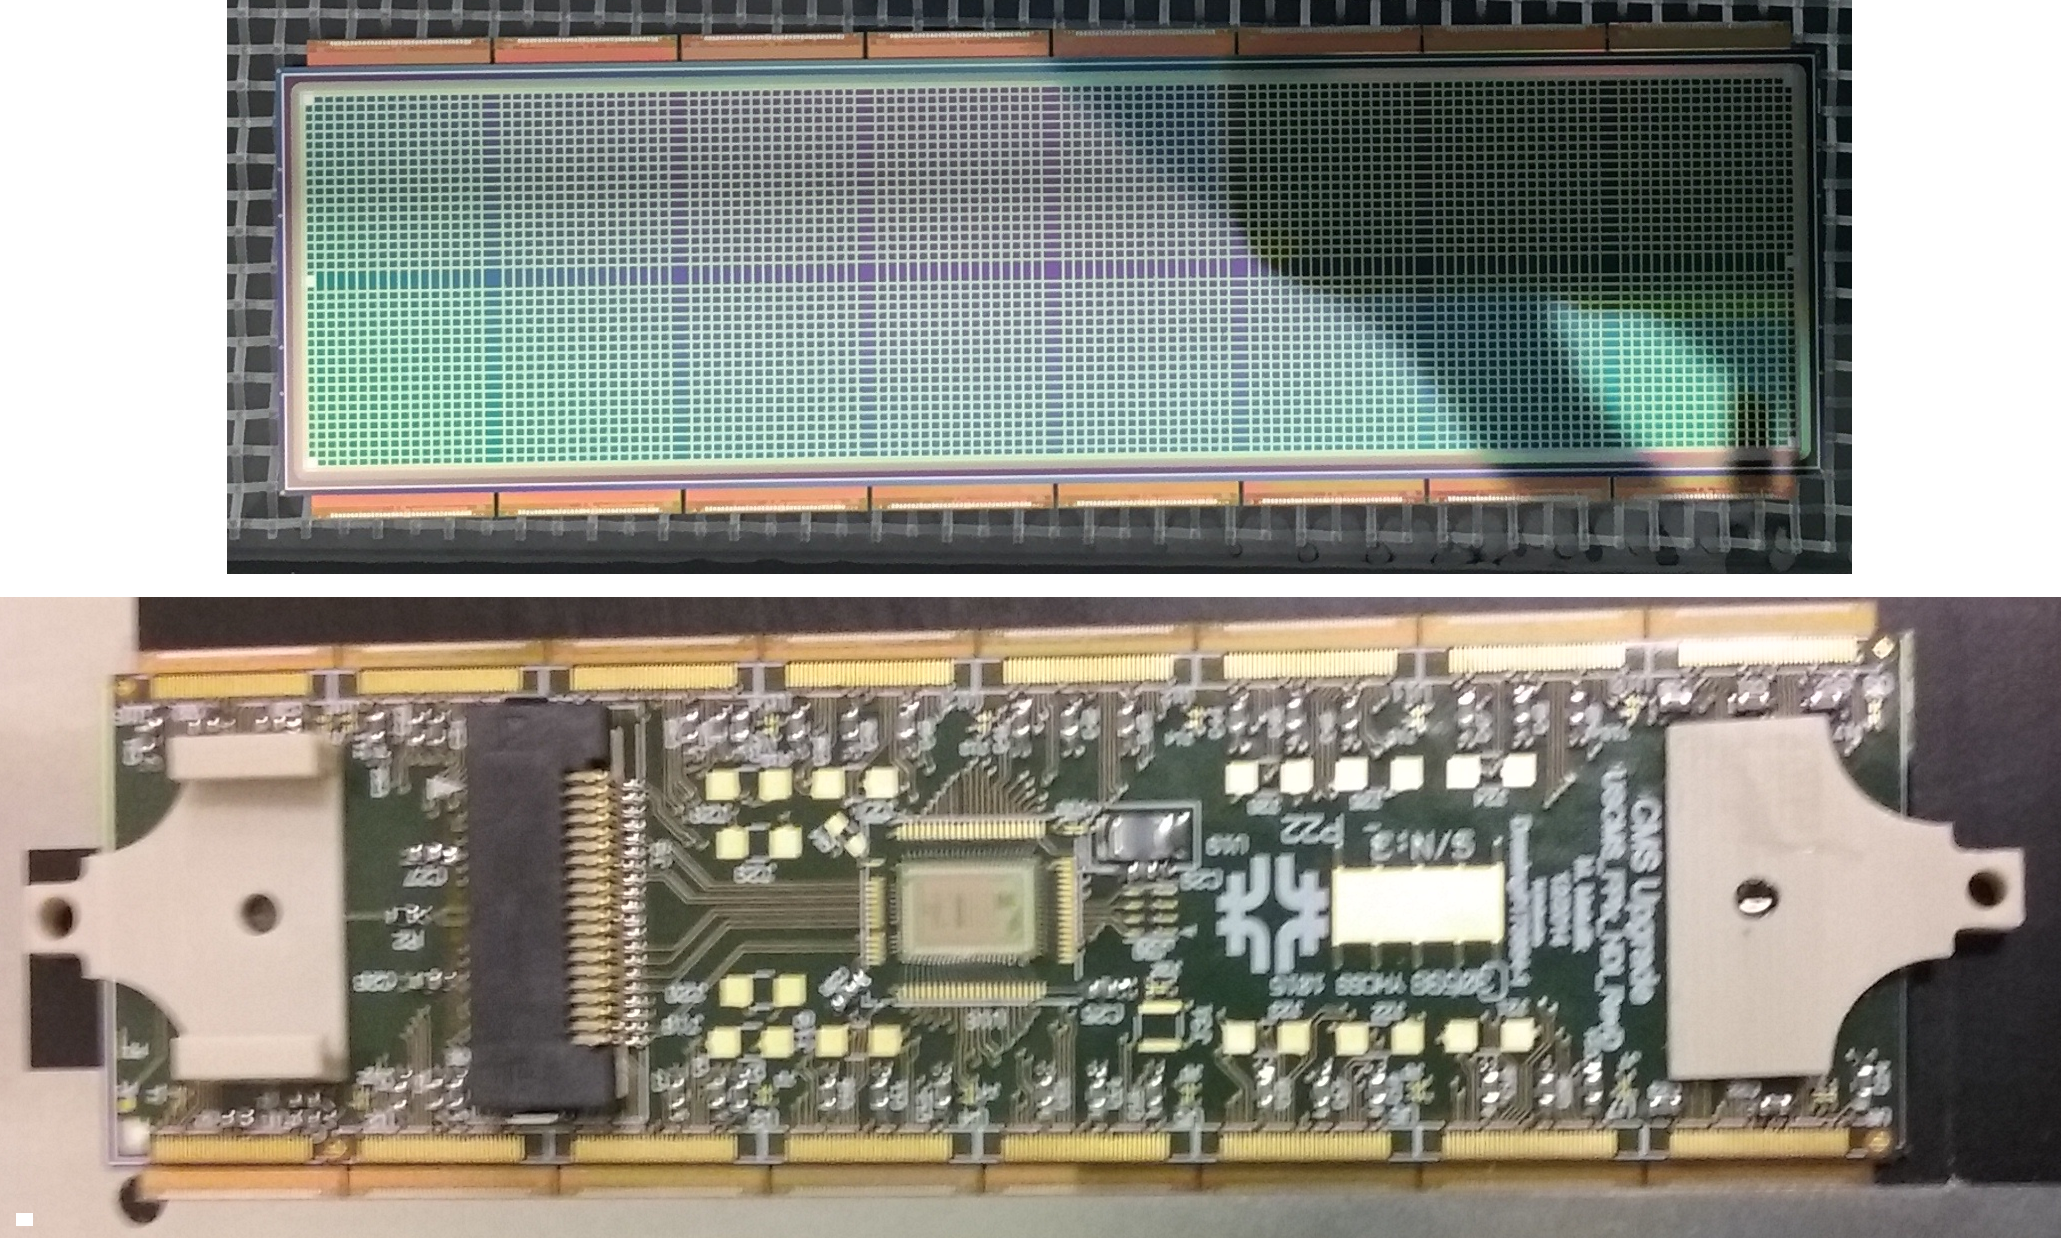
\includegraphics[width=0.63\textwidth]{pixel/bbm_hdi}
  \caption[FPix module structure.]{Top: FPix module structure; The bare silicon sensor is bump-bonded to the ROCs to form the BBM; then the HDI is glued on top of the BBM and wirebonded to the ROCs. Bottom: pictures of actual BBM and HDI.}\label{fig:fpix_struc}
\end{figure}

The current CMS pixel detector is composed of 1184 pixel modules in the BPIX sector with a total 79 million of pixels; the FPix sector contains 672 with approximately 45 million pixels. Figure \ref{fig:fpix_struc} shows a schematic view of the FPix modules structure. The n$^{+}$-in-n \ti{Silicon sensor} is Bump-Bonded to the 16 ROC to form the detector unit known as \ti{Bump-Bonded Module} (BBM) with 66560 pixels. The \ti{High Density Interconnect} (HDI) is glued on top of the BBM and wirebonded to the ROCs to provide them the required signals and power. The modules are attached to the support structure using the end holders glued to the HDI.

\section{FPix module assembly}

The construction of the modules for the current FPix system was divided between two sites located at Purdue University and at UNL; testing facilities were located at the University of Kansas and Fermi National Accelerator Laboratory (Fermilab). The integration facility was based at Fermilab. 

The BBM was prepared by a commercial vendor, while the HDI was populated at Fermilab, with all the electronic components like resistors, capacitors and the central component known as \ti{Token Bit Manager} (TBM), which is in charge of managing the information coming from the silicon sensors and going to the ROCs. Both BBM and HDI were sent to the assembly sites ready to be glued together.  


\begin{figure}[!h]
  \centering
  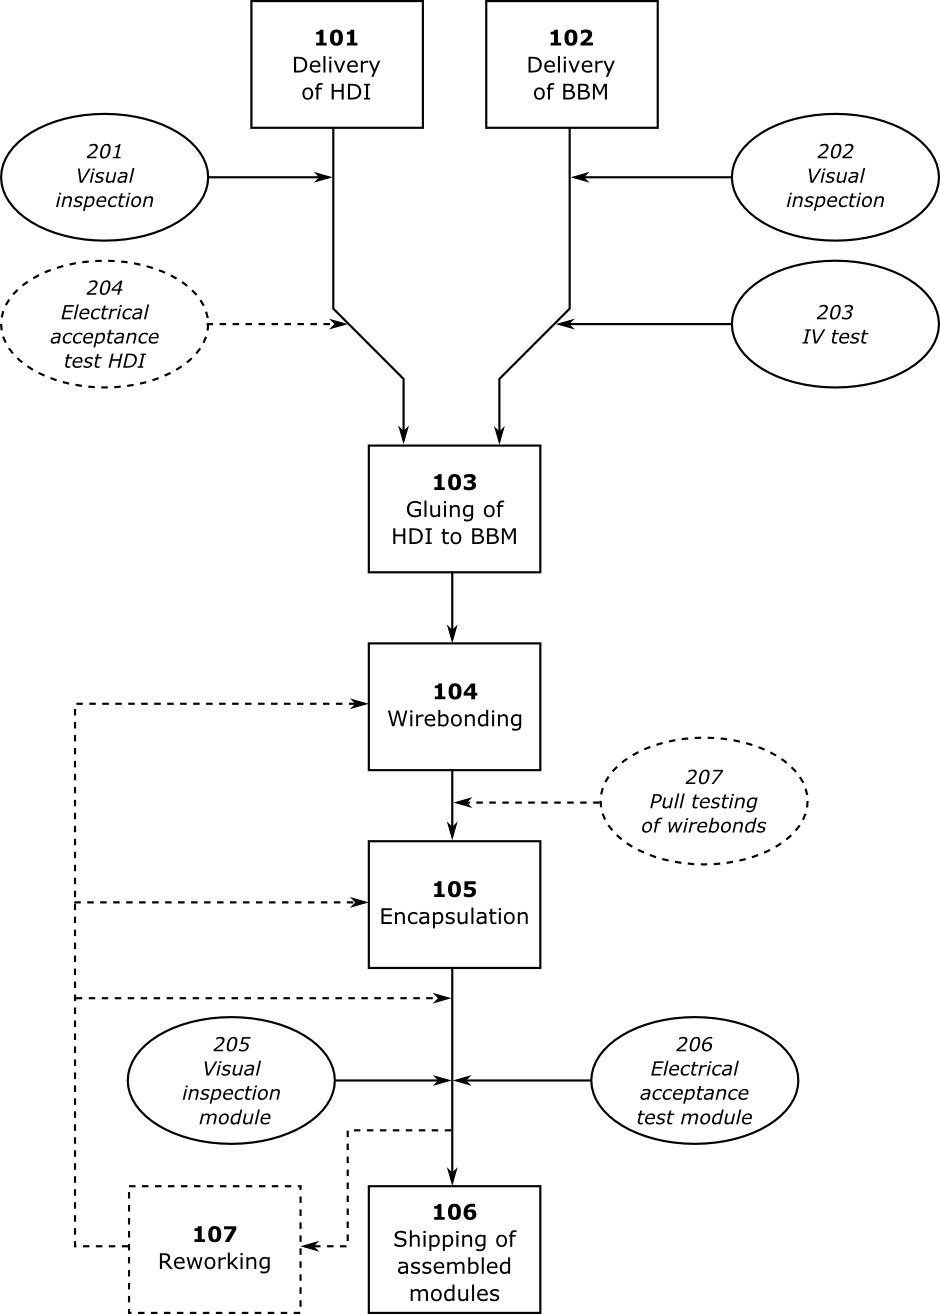
\includegraphics[width=0.7\textwidth]{pixel/UNLworkflow}
  \caption[UNL module assembly work flow.]{UNL module assembly work flow. Dashed lines represent occasional quality testing and reworking procedures; 10X numbers represent the stage within the assembly procedure while 20X numbers represent testing stages along the assembly procedure.}\label{fig:unlworkflow}
\end{figure}


The module production procedure was designed according to a production line structure. Figure \ref{fig:unlworkflow} shows the work flow followed at the UNL assembly site. Once the BBM and HDI arrive, they are submitted to visual inspection looking for defects, scratches, dents or short circuits. Modules passing the visual inspection are tested for electrical acceptance and performance. BBM and HDI are then glued employing robotic a pick-and-place machine that integrates optic tools, pattern recognition algorithms, and glue dispensing; the semi-automated gluing process improves the uniformity of the technique. After 10 hours of curing, glued modules are moved to the wirebonding station where ROCs and HDI are electrically connected employing semi-automated ultrasonic wirebongding machines; occasionally, some of the wires are pull tested for quality control. After this step, modules are fully functional, hence, a basic functionality test is done at a subset of modules to control the manufacturing process.    

In the next stage, the wirebonds are encapsulated with an elastomeric compound (\ti{Sylgard}) in order to protect them against mechanical damage and electrical shorts; the encapsulation process is performed employing the robotic pick-and-place machine which also integrates the encapsulant dispensing system. Once the encapsulation ends, modules are mounted on module holders and submitted to a head cycle to cure the sylgard.    

The module assembly sites were also responsible for the testing and characterization of the assembled pixel modules. That testing included visual inspection, electrical acceptance, performance testing under controlled temperature conditions that simulate the expected operational conditions; in case of any necessary reworking, the modules were returned to the appropriate stage.

In the final stage, the assembled and tested modules were shipped to the University of Kansas for further characterization.  

Each stage in the assembly procedure is documented in a ~\ti{Standard Operating Procedure} (SOP) document that describes the procedures to be followed by the operator. The full set of SOPs can be found in Reference \cite{unl_sop}.     

In the following sections, a detailed description of the gluing and encapsulation stages will be presented. The full set of tools was designed by Dr. Frank Meier Aeschbacher. 

\subsection{Pick and place machine setup}\label{sec:setup}

Figure \ref{fig:setup} shows the full setup used to perform the gluing and encapsulation steps. The gantry used in the setup is a custom made \ti{AGS15000 Series Gantry}, fabricated by Aerotech \cite{aerotech}, which offers translational motion in 3D ensuring coverage of any position in the work field; in addition, rotational motion is provided in the \ti{gantry head} in the usual x-y plane (gantry table plane).

\begin{figure}[!h]
  \centering
  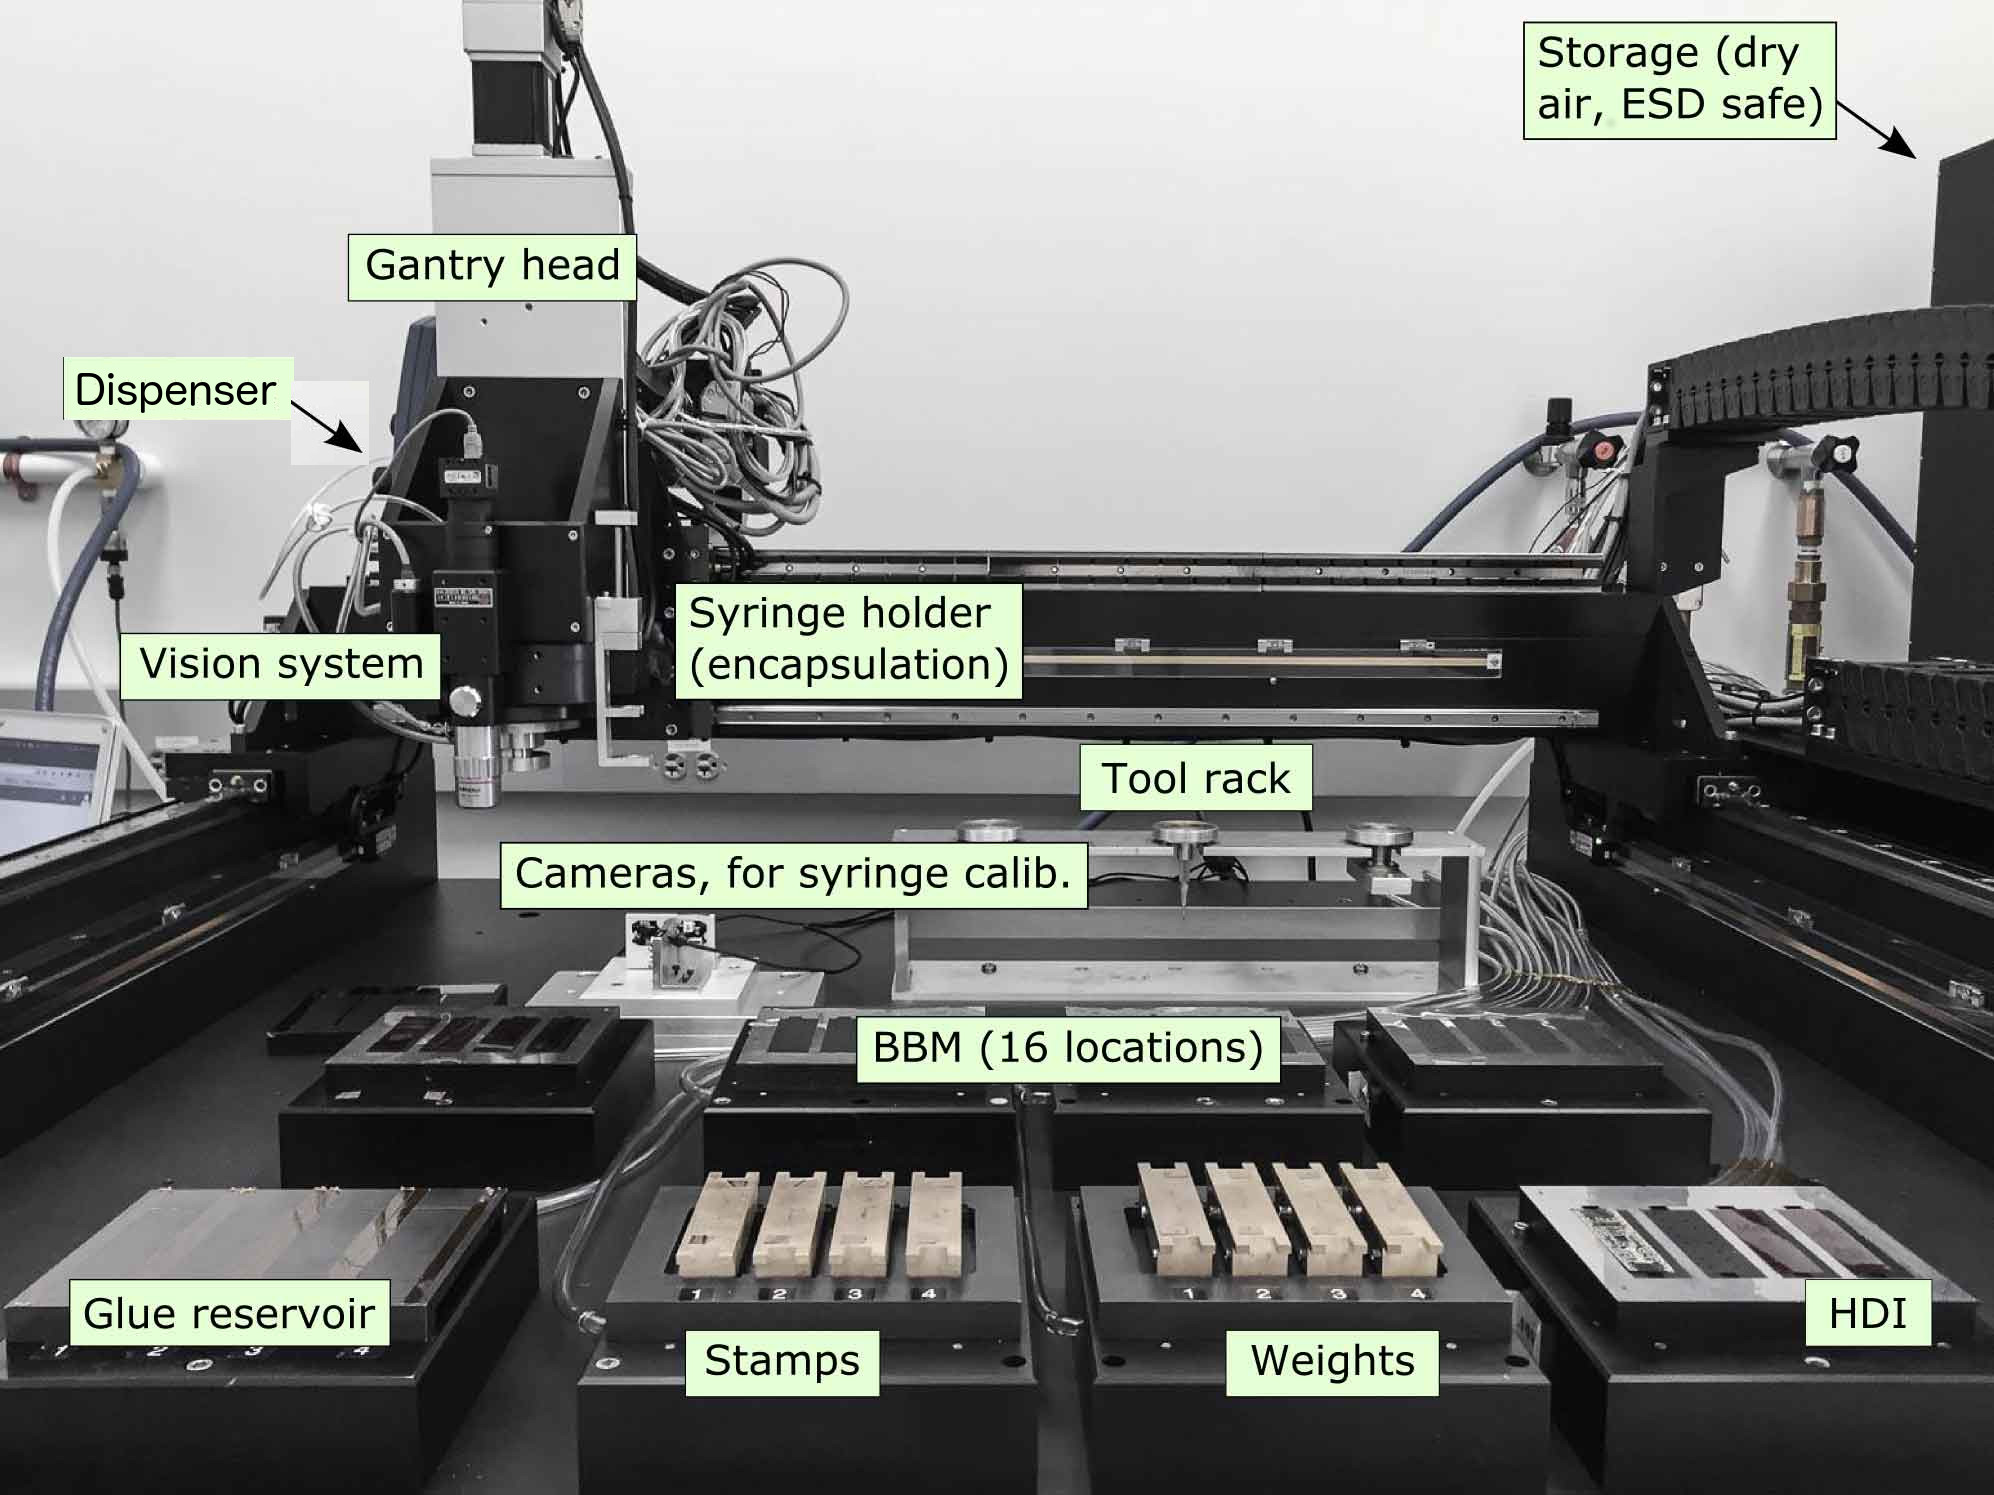
\includegraphics[width=\textwidth]{pixel/gantryFull16labeled}
  \caption[Full gluing and encapsulation setup]{Full gluing and encapsulation setup. }\label{fig:setup}
\end{figure}

A set of eight hard-anodized aluminum chucks, composed of a \ti{base chuck} and a \ti{plate chuck} each, henceforth chuck and plate respectively, were designed to house the parts and tools needed along the gluing process; Figure \ref{fig:chuck} shows the details of a chuck.      

\begin{figure}[!h]
  \centering
  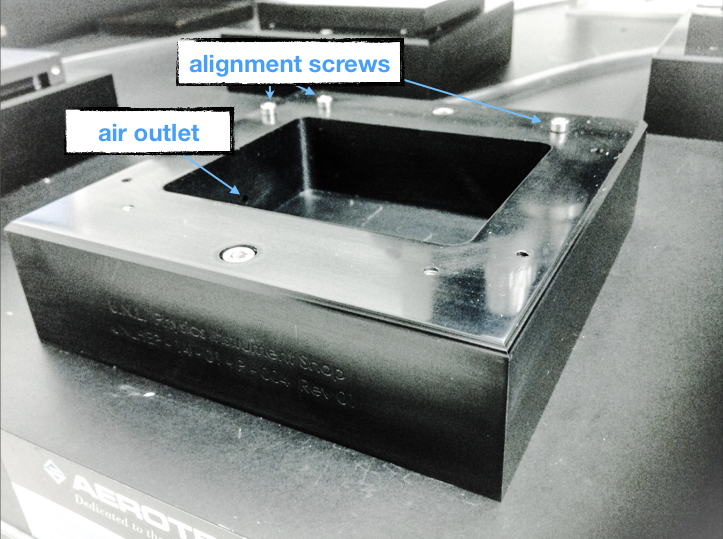
\includegraphics[width=0.48\textwidth]{pixel/chuck}
  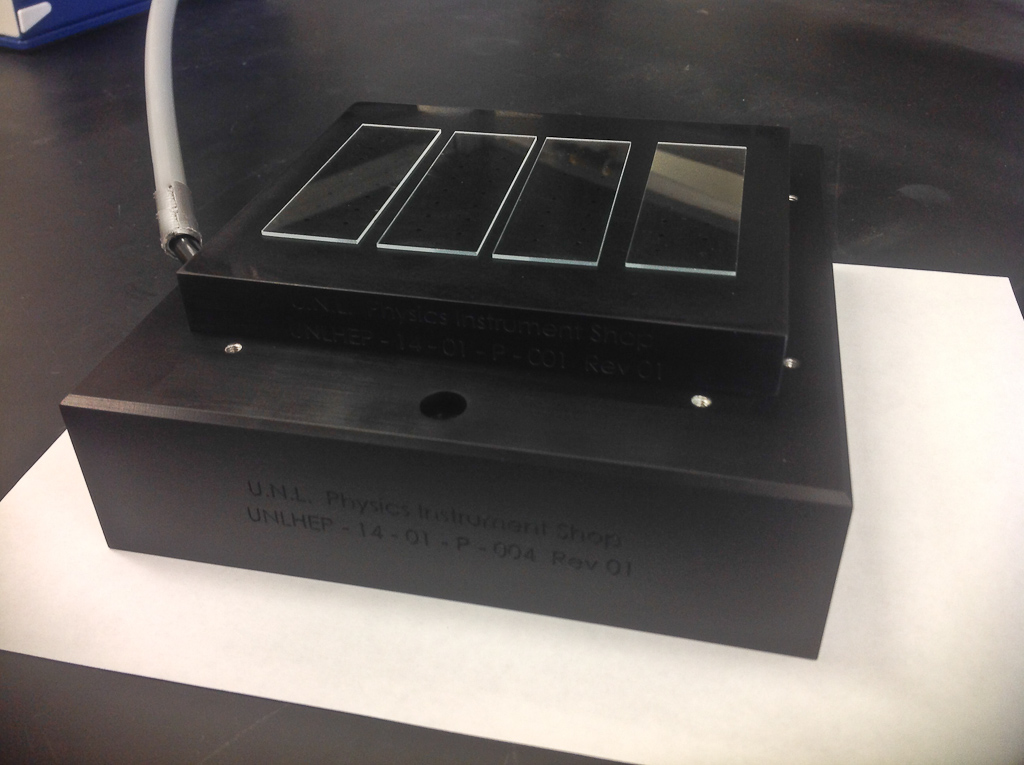
\includegraphics[width=0.48\textwidth]{pixel/chucksAnodized}
  \caption[Bare and full chucks]{Left: Chuck detailed internal view. Right: full chuck housing glass slides. The vacuum connection is visible on the left.}\label{fig:chuck}
\end{figure}

Each chuck is connected to an independent vacuum line such that the plate is held fixed; both pieces are polished to seal the vacuum with no use of O-rings. The three screws serve as references for aligning the plates with the chucks. There are four types of plates; HDI/BBM plate, the glue reservoir plate, stamp plate, weight plate.

\subsubsection*{Chucks}

Four chucks are used to accommodate sixteen BBMs (four per plate); the holes in the BBM/HDI plate (see Figure \ref{fig:bbm_hdi_plates}) are intended to hold the BBM/HDI safely fixed to the plate by the action of the vacuum, while the stencil (100 $\mu$m in thickness) allows for a very accurate positioning of the BBM/HDI; it is thin enough that the alignment is controlled by the edges of the ROC and no force is applied to the sensor.     

\begin{figure}[!h]
  \centering
  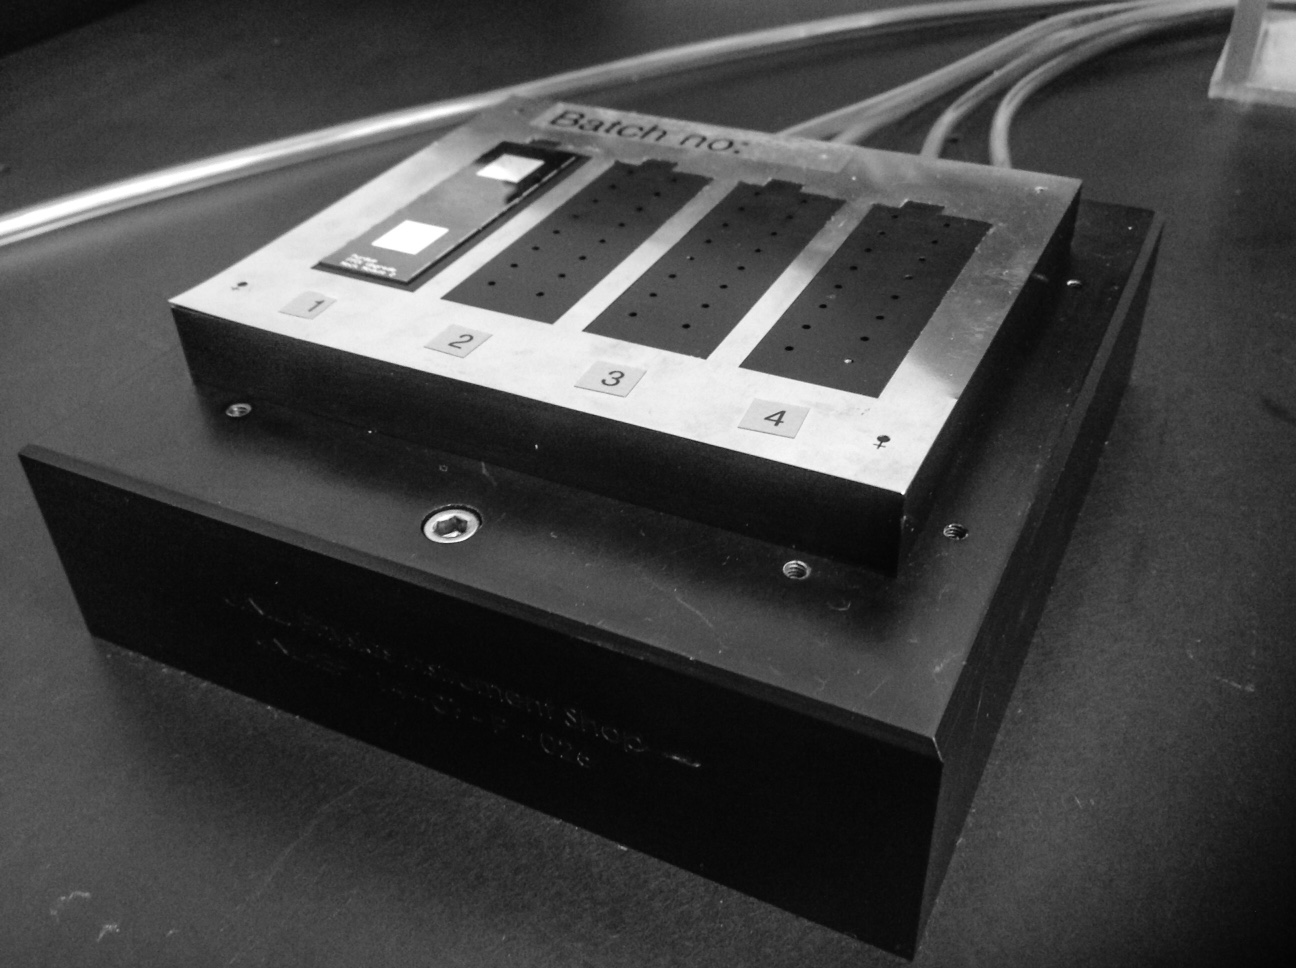
\includegraphics[width=0.32\textwidth, height= 0.32\textwidth]{pixel/bbm_chuck}
  \includegraphics[width=0.32\textwidth, height= 0.32\textwidth]{pixel/hdi_plate_adj}
  \includegraphics[width=0.32\textwidth, height= 0.32\textwidth]{pixel/hdi_stencil}
  \caption[BBM/HDI plate]{Left: BBM/HDI plate with a mock module that reproduces the BBM features. Center: the pockets in the top and bottom sides accommodate the module holders. Right: bare HDI and BBM showing the alignment provided by the stencil.}\label{fig:bbm_hdi_plates}
\end{figure}

One chuck is dedicated to accommodate four HDIs. Although BBM/HDI plates have the same design, the HDI chuck has four independent pockets instead of only a big one, in order to enable the release of one HDI at a time; hence, it is connected to 4 vacuum lines. That is not required for the BBMs because they are not moved from their original location. An additional adjustment was made to the HDI plate in response to the HDI back surface which is not totally flat but has irregularities; these irregularities caused vacuum leaks that were addressed by adding a kapton tape layer to the HDI plate, as shown in the center of Figure~\ref{fig:bbm_hdi_plates}. The tracks make sure that the vacuum action and the tape flexibility ensures the sealing.    

One chuck holds the \ti{glue reservoir} plate, as shown in Figure \ref{fig:glue_reservoir}. Each of the four reservoirs is a pocket just 100 $\mu$m deep, suitable for retaining sufficient glue to be applied to the BBM.  

\begin{figure}[!h]
  \centering
  %\includegraphics[width=0.4\textwidth, height= 0.4\textwidth]{pixel/glue_plate_adj}
  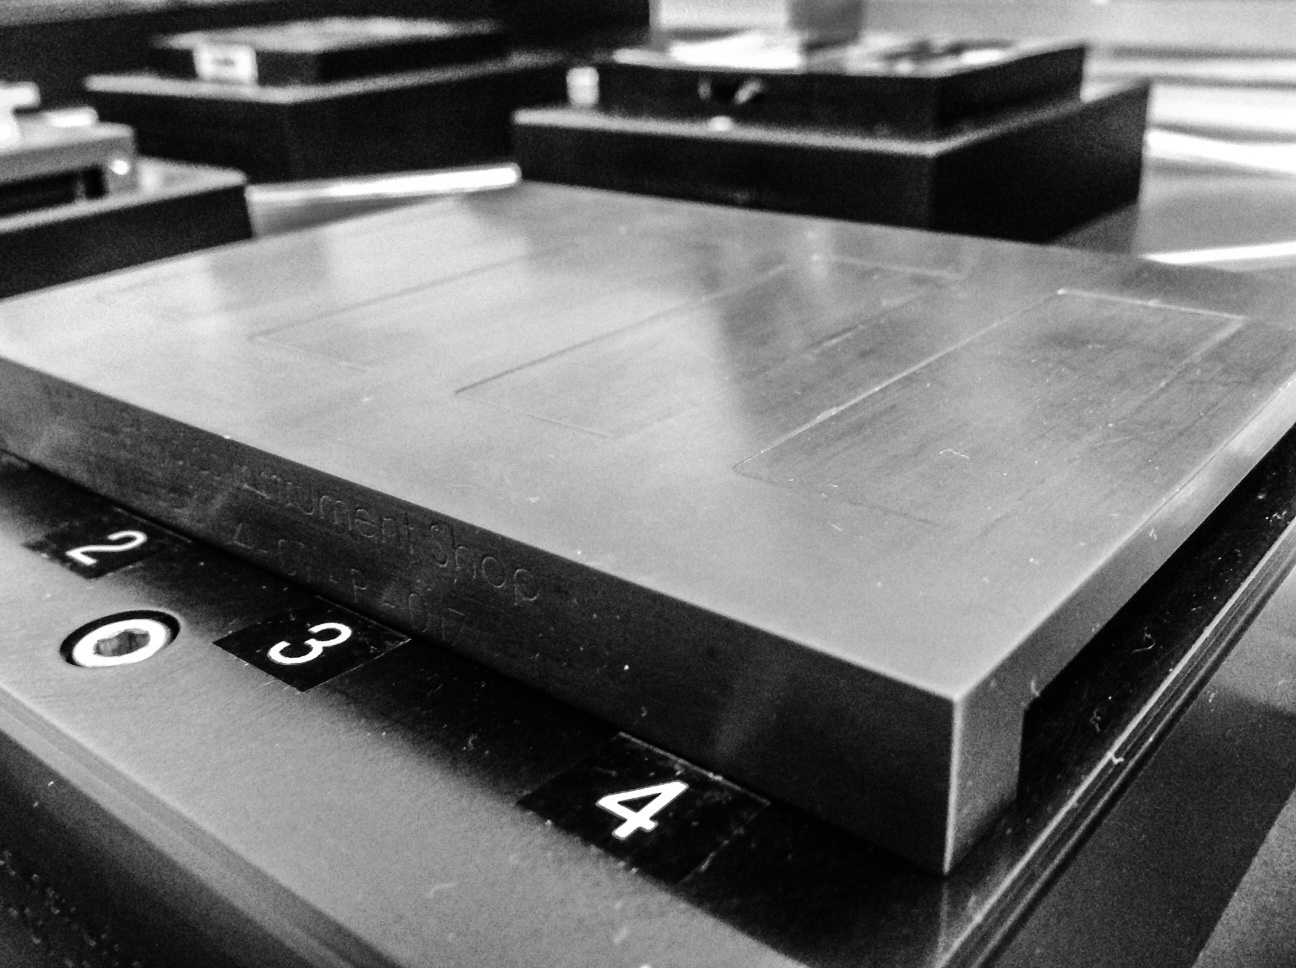
\includegraphics[width=0.5\textwidth]{pixel/glue_reservoir}
  \caption[Glue reservoir plate]{Glue reservoir plate. The four pockets are 100 $\mu$m deep. }\label{fig:glue_reservoir}
\end{figure}

The remaining two chucks house the \ti{stamp plate} and the \ti{weight plate} which in turn house the \ti{stamp tools} and the \ti{weight tools} as shown in Figure~\ref{fig:st_wt_plates}. 

\begin{figure}[!h]
  \centering
  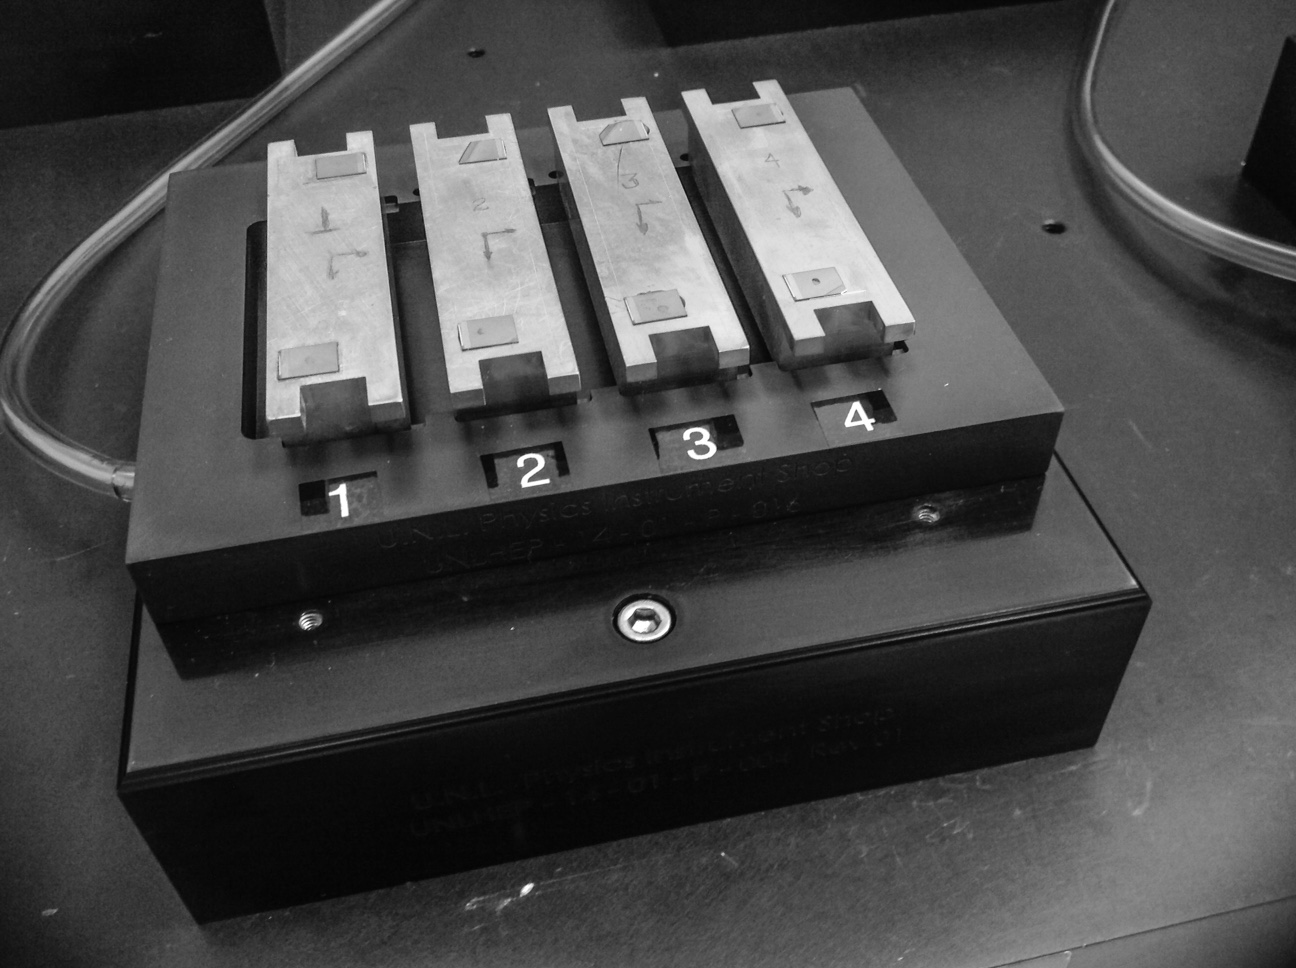
\includegraphics[width=0.45\textwidth]{pixel/chuck_stamps}
  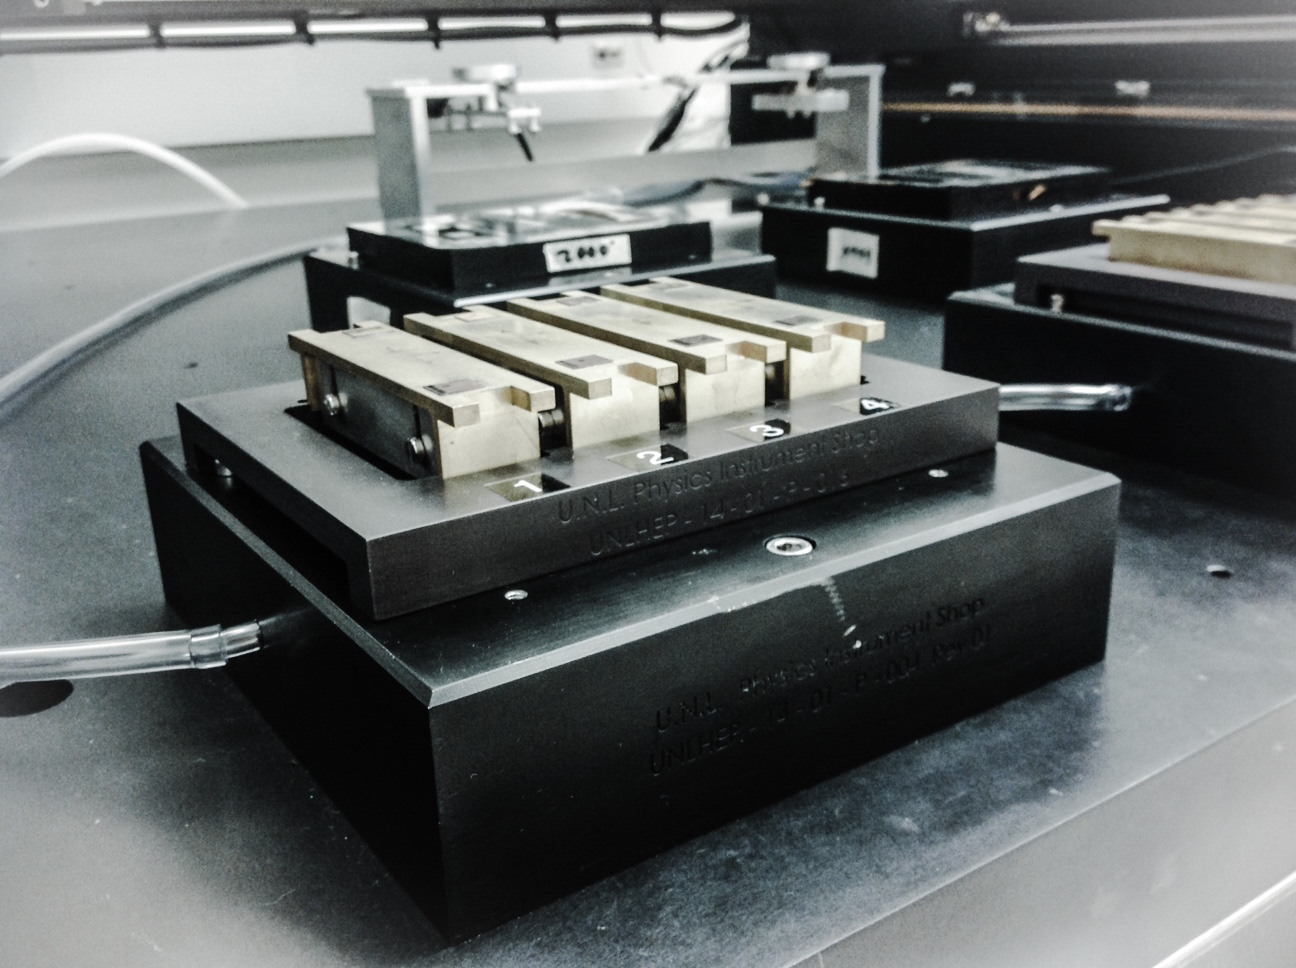
\includegraphics[width=0.45\textwidth]{pixel/chuck_weights}
  \caption[Stamp and Weight tools in chucks]{Chucks housing stamp tools(left) and weight tools(right).}\label{fig:st_wt_plates}
\end{figure}

\subsubsection*{Stamp and weight tools}

\begin{figure}[!h]
  \centering
  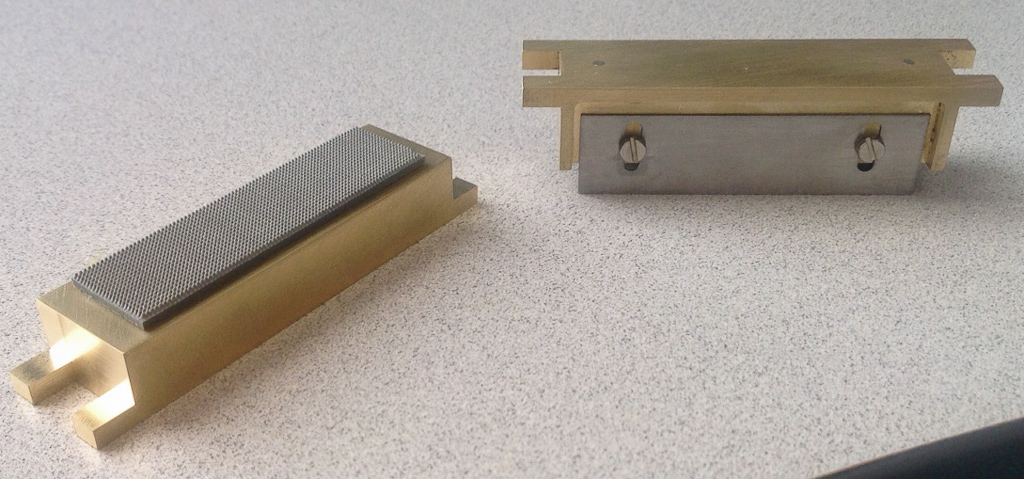
\includegraphics[width=0.45\textwidth, height=0.35\textwidth]{pixel/tools}
  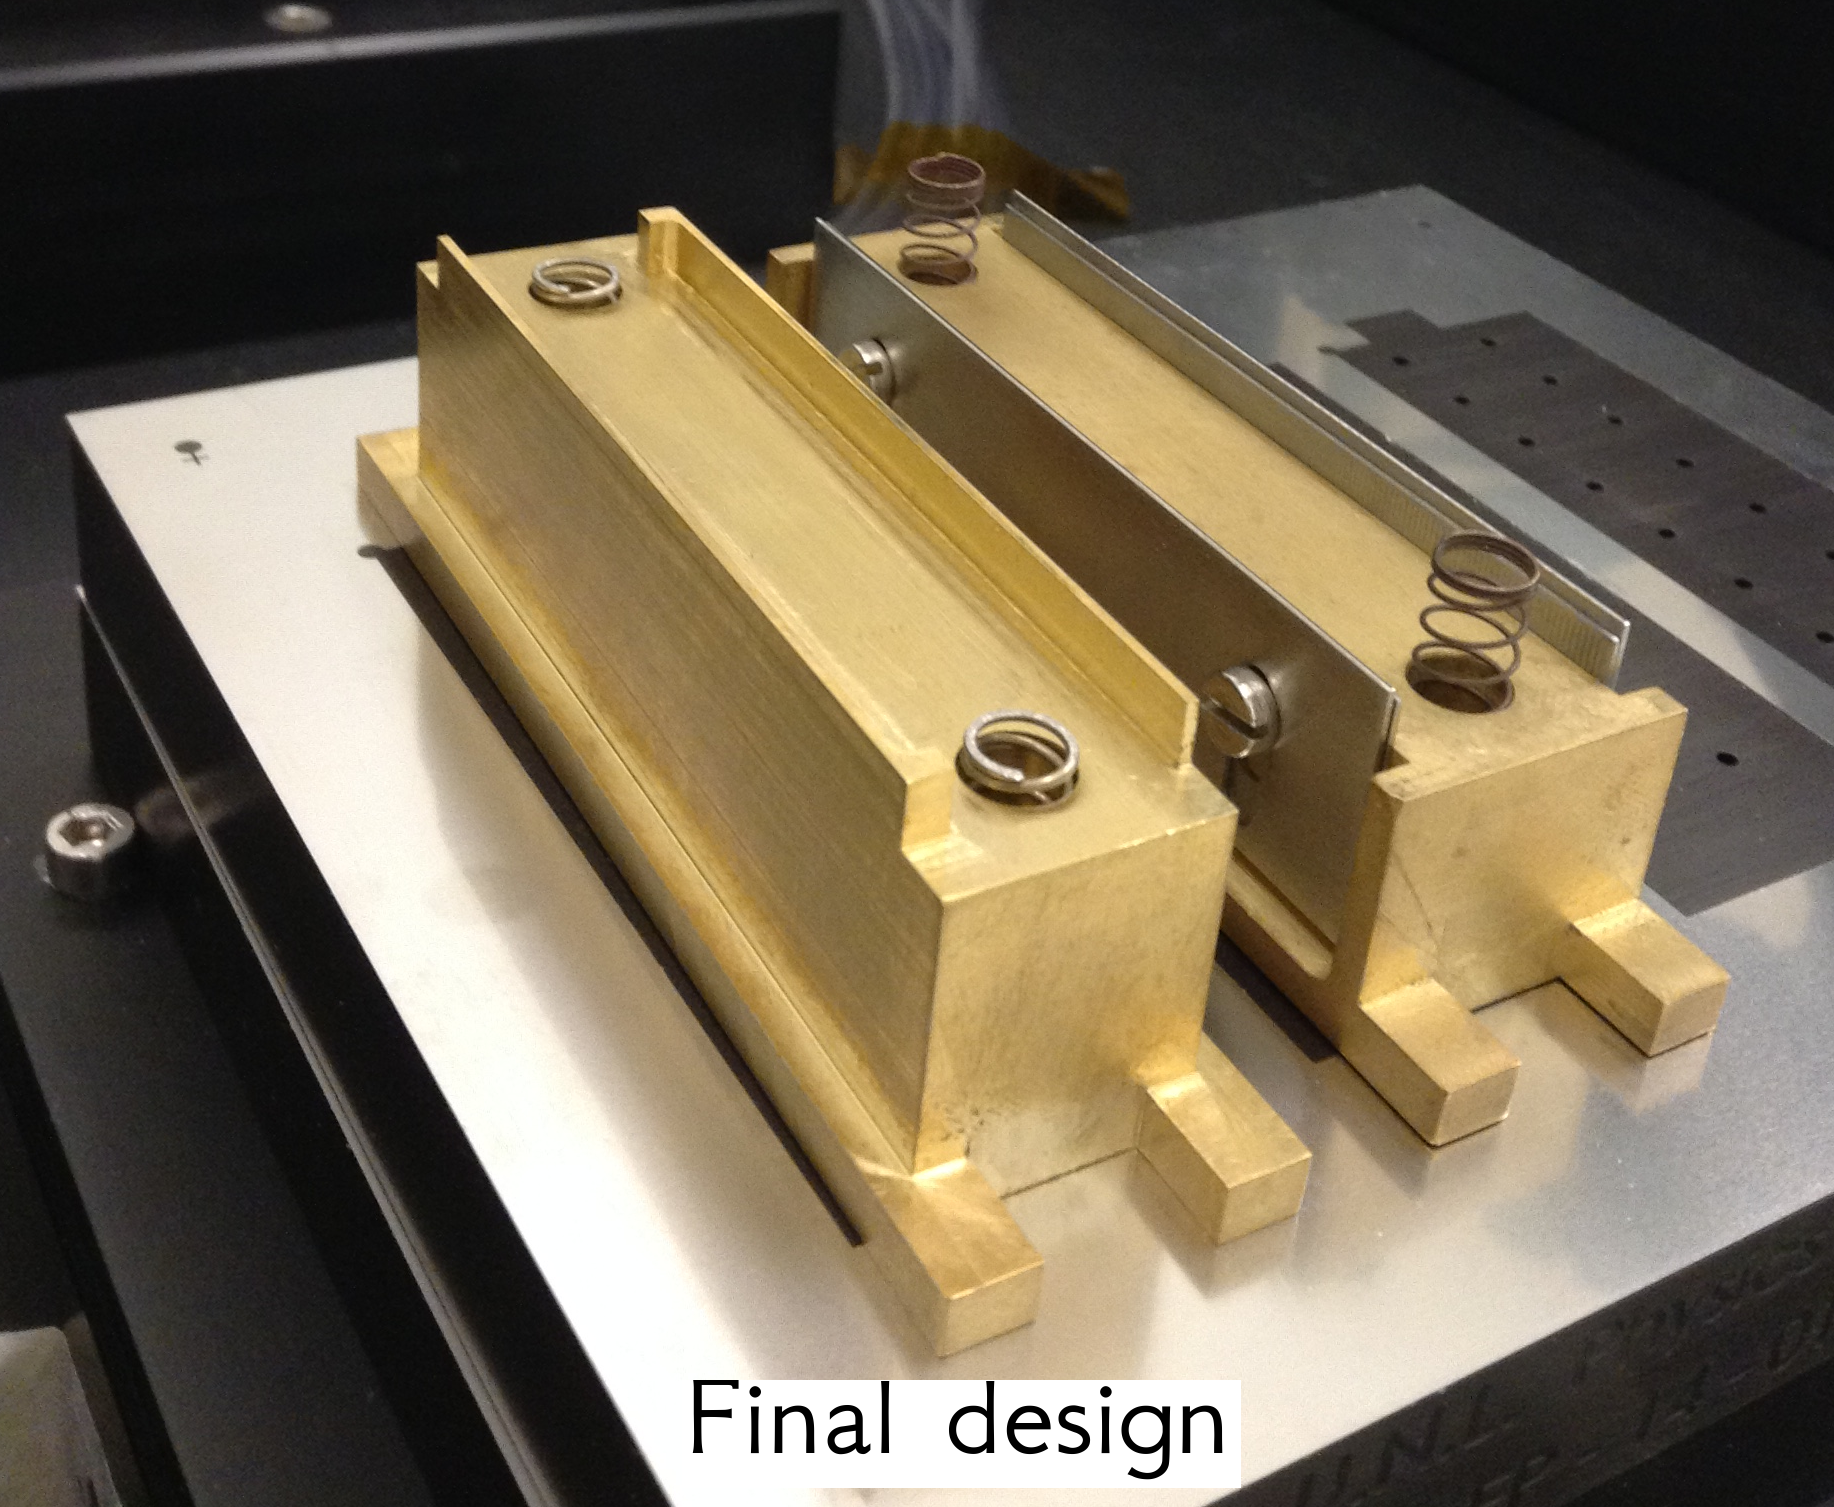
\includegraphics[width=0.45\textwidth, height=0.35\textwidth]{pixel/tools2}
  \caption[Stamp and Weight tools]{Stamp and weight tools. Both tools are made of brass; the stamp tool includes a rubber stamp while the weight tool includes four stainless steel blades to apply force while curing. The final weight tool design eliminates the blades (right).}\label{fig:st_wt}
\end{figure}

Stamp and weight tools are a set of custom made tools, all produced by the UNL Physics department machine shop (see Figure~\ref{fig:st_wt}). The very first design of the weight tool included four stainless steel blades and two springs; the blades matched the rows of 8 ROC bond pads on the HDI to apply force while curing. The springs apply force to the module end holders on the HDI. The final design of the tool eliminates the issues associated with the alignment of the blades, by integrating them into the design in the form of narrow blade-like brass edges. The weight tools were made with 260 g of brass.      

The stamp tool is composed of a brass piece of 200 g and a rubber stamp piece attached to the bottom side of the brass piece; it is used to pick the glue from the glue reservoir and then stamp it over the BBM. An extensive testing process was performed in order to determine the most appropriate features of the gluing strategy. Figure~\ref{fig:stamp_pattern} shows the four stamp patterns tested and a picture of the first two attached to the stamp tools; the variations of the stamp pattern design were based on the results of testing for:

\begin{figure}[!h]
  \centering  
  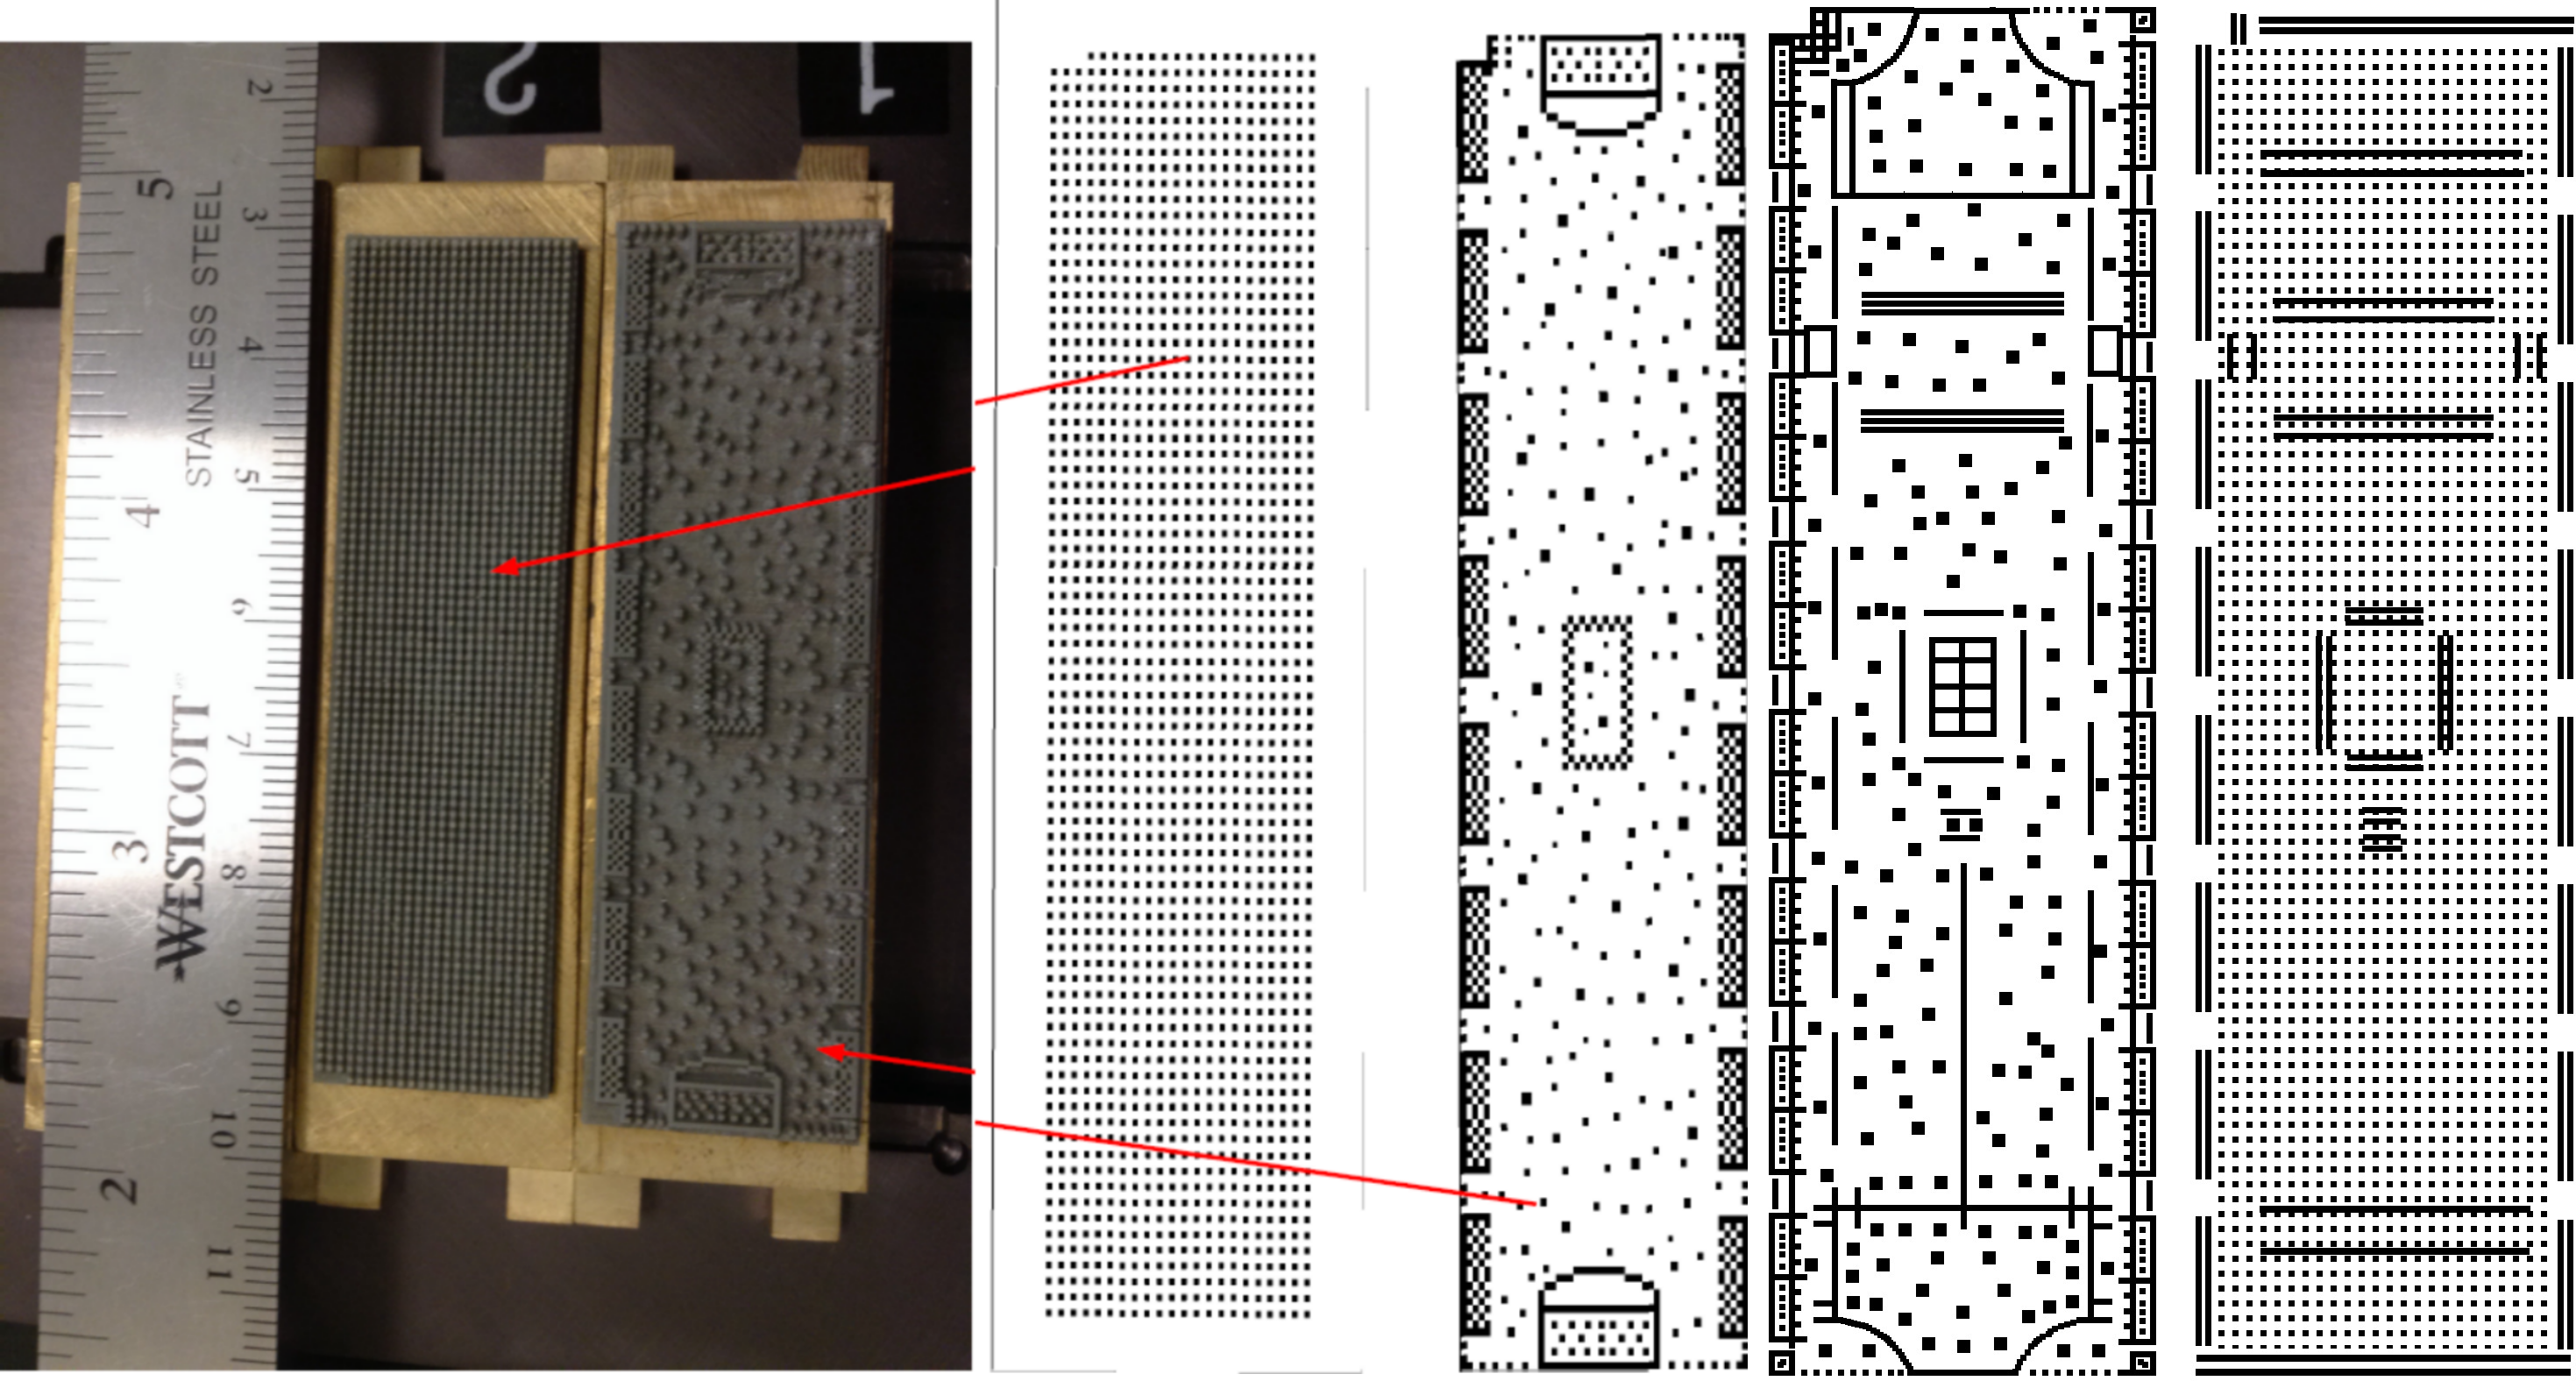
\includegraphics[width=0.3\textwidth,height=0.4\textwidth]{pixel/stamps}
  
\includegraphics[width=0.12\textwidth,height=0.4\textwidth]{pixel/stamp1}
  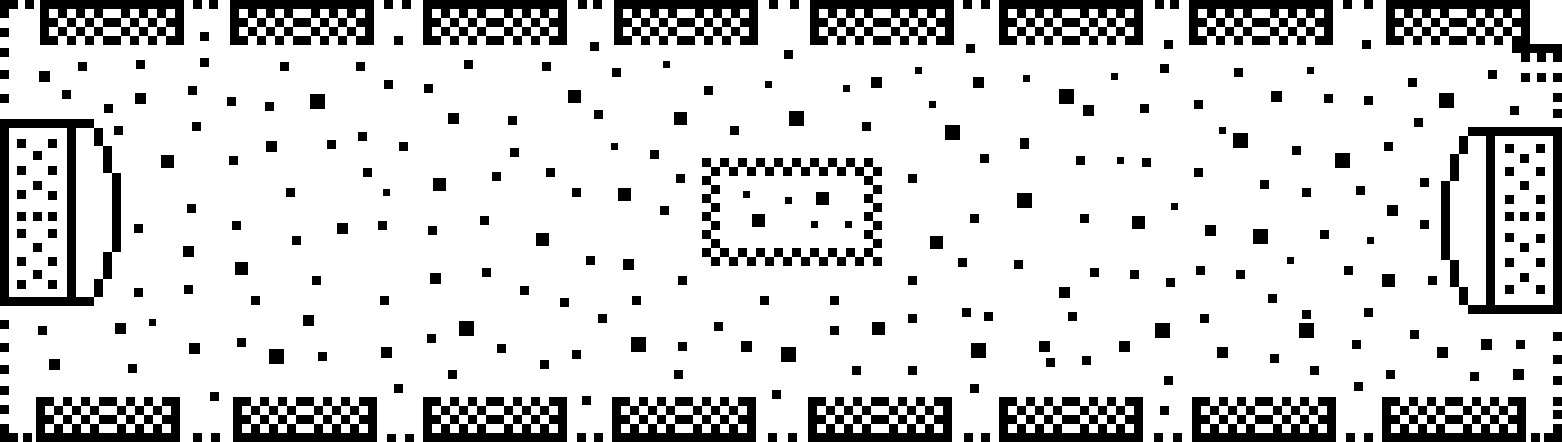
\includegraphics[width=0.12\textwidth,height=0.4\textwidth]{pixel/stamp2}
  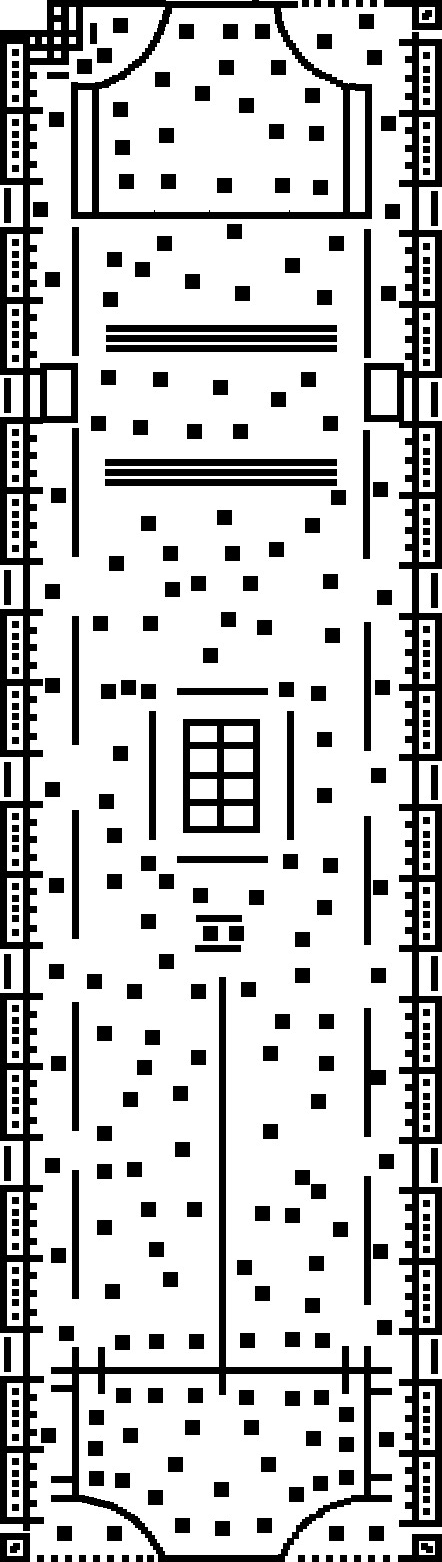
\includegraphics[width=0.12\textwidth,height=0.4\textwidth]{pixel/stamp3}
  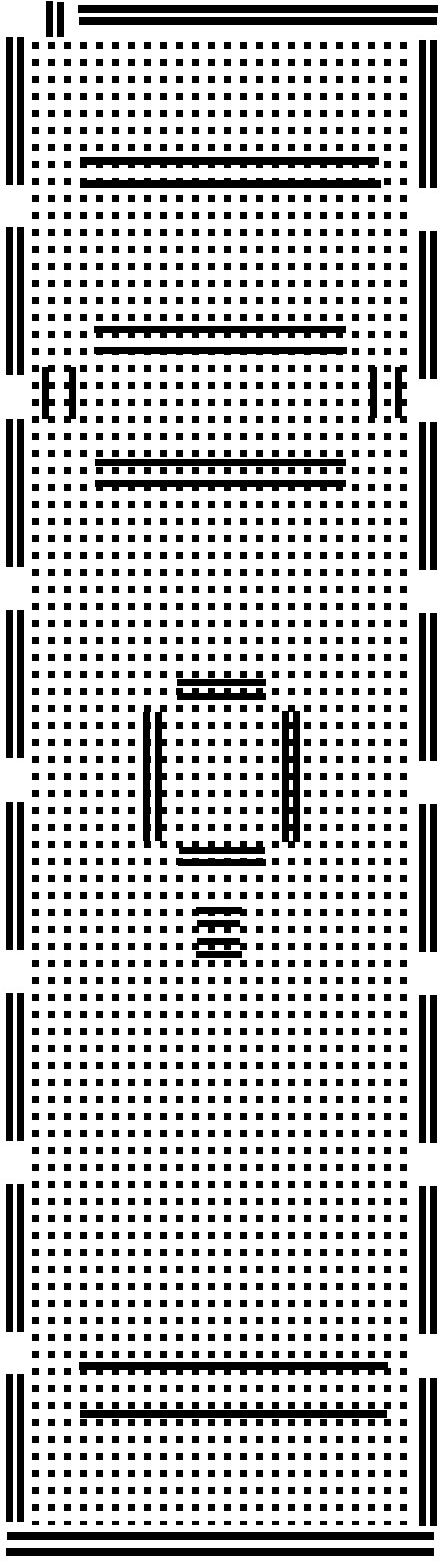
\includegraphics[width=0.12\textwidth,height=0.4\textwidth]{pixel/stamp4}
  \caption[Stamp patterns]{Stamp patterns evaluated along the glue testing process; the picture on the left show the first two versions mounted on the stamp tool while the final version is on the right.}\label{fig:stamp_pattern}
\end{figure}

\bit
  \begin{figure}[!h]
  \centering
  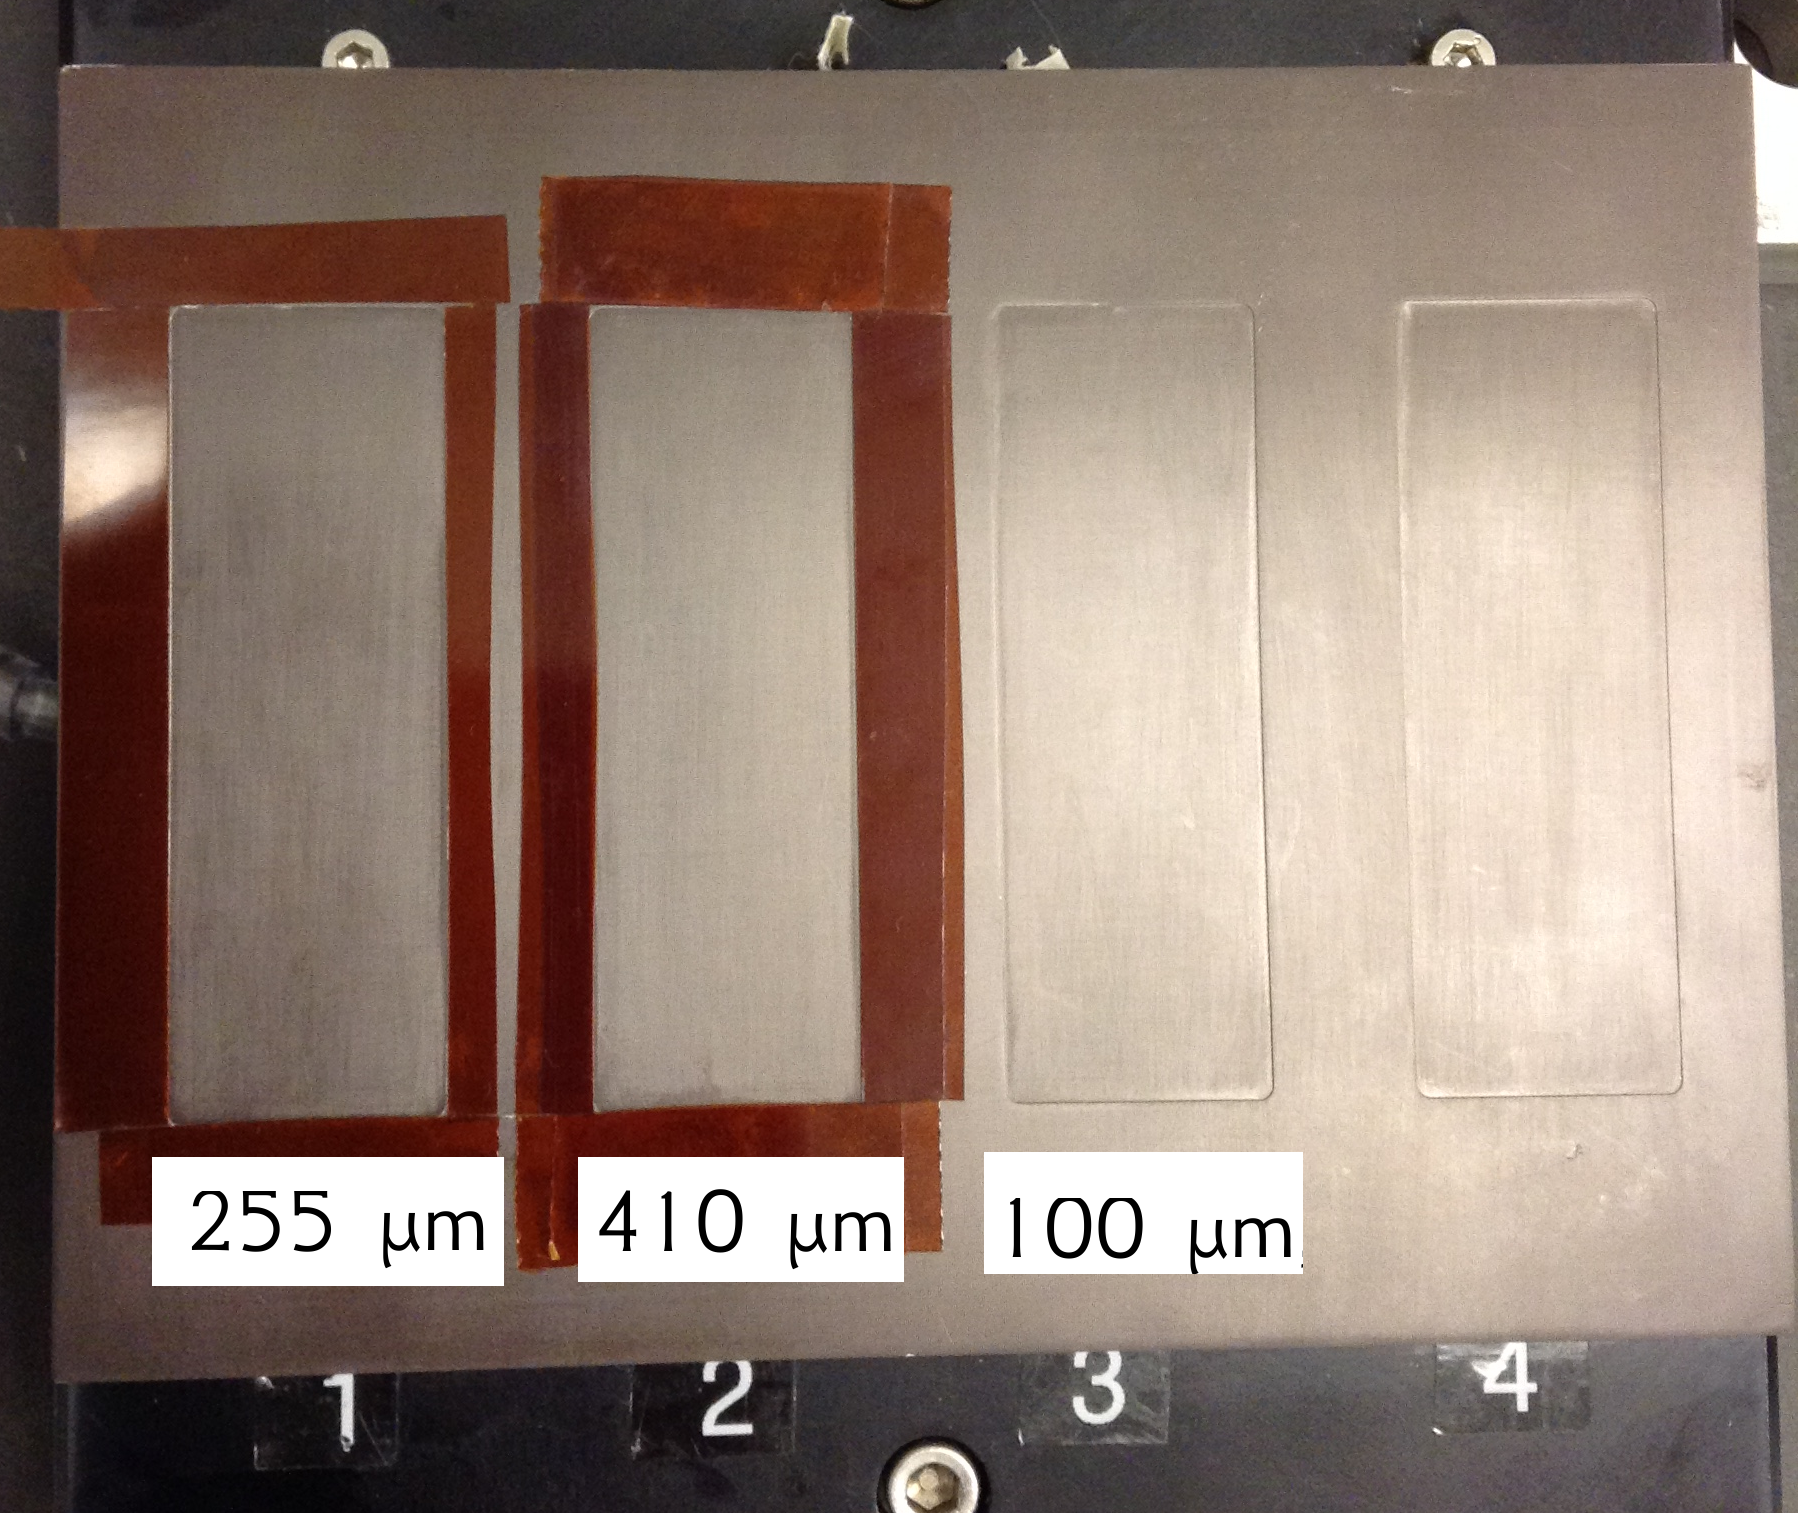
\includegraphics[width=0.4\textwidth, height=0.4\textwidth]{pixel/reservoir_depth_test}
  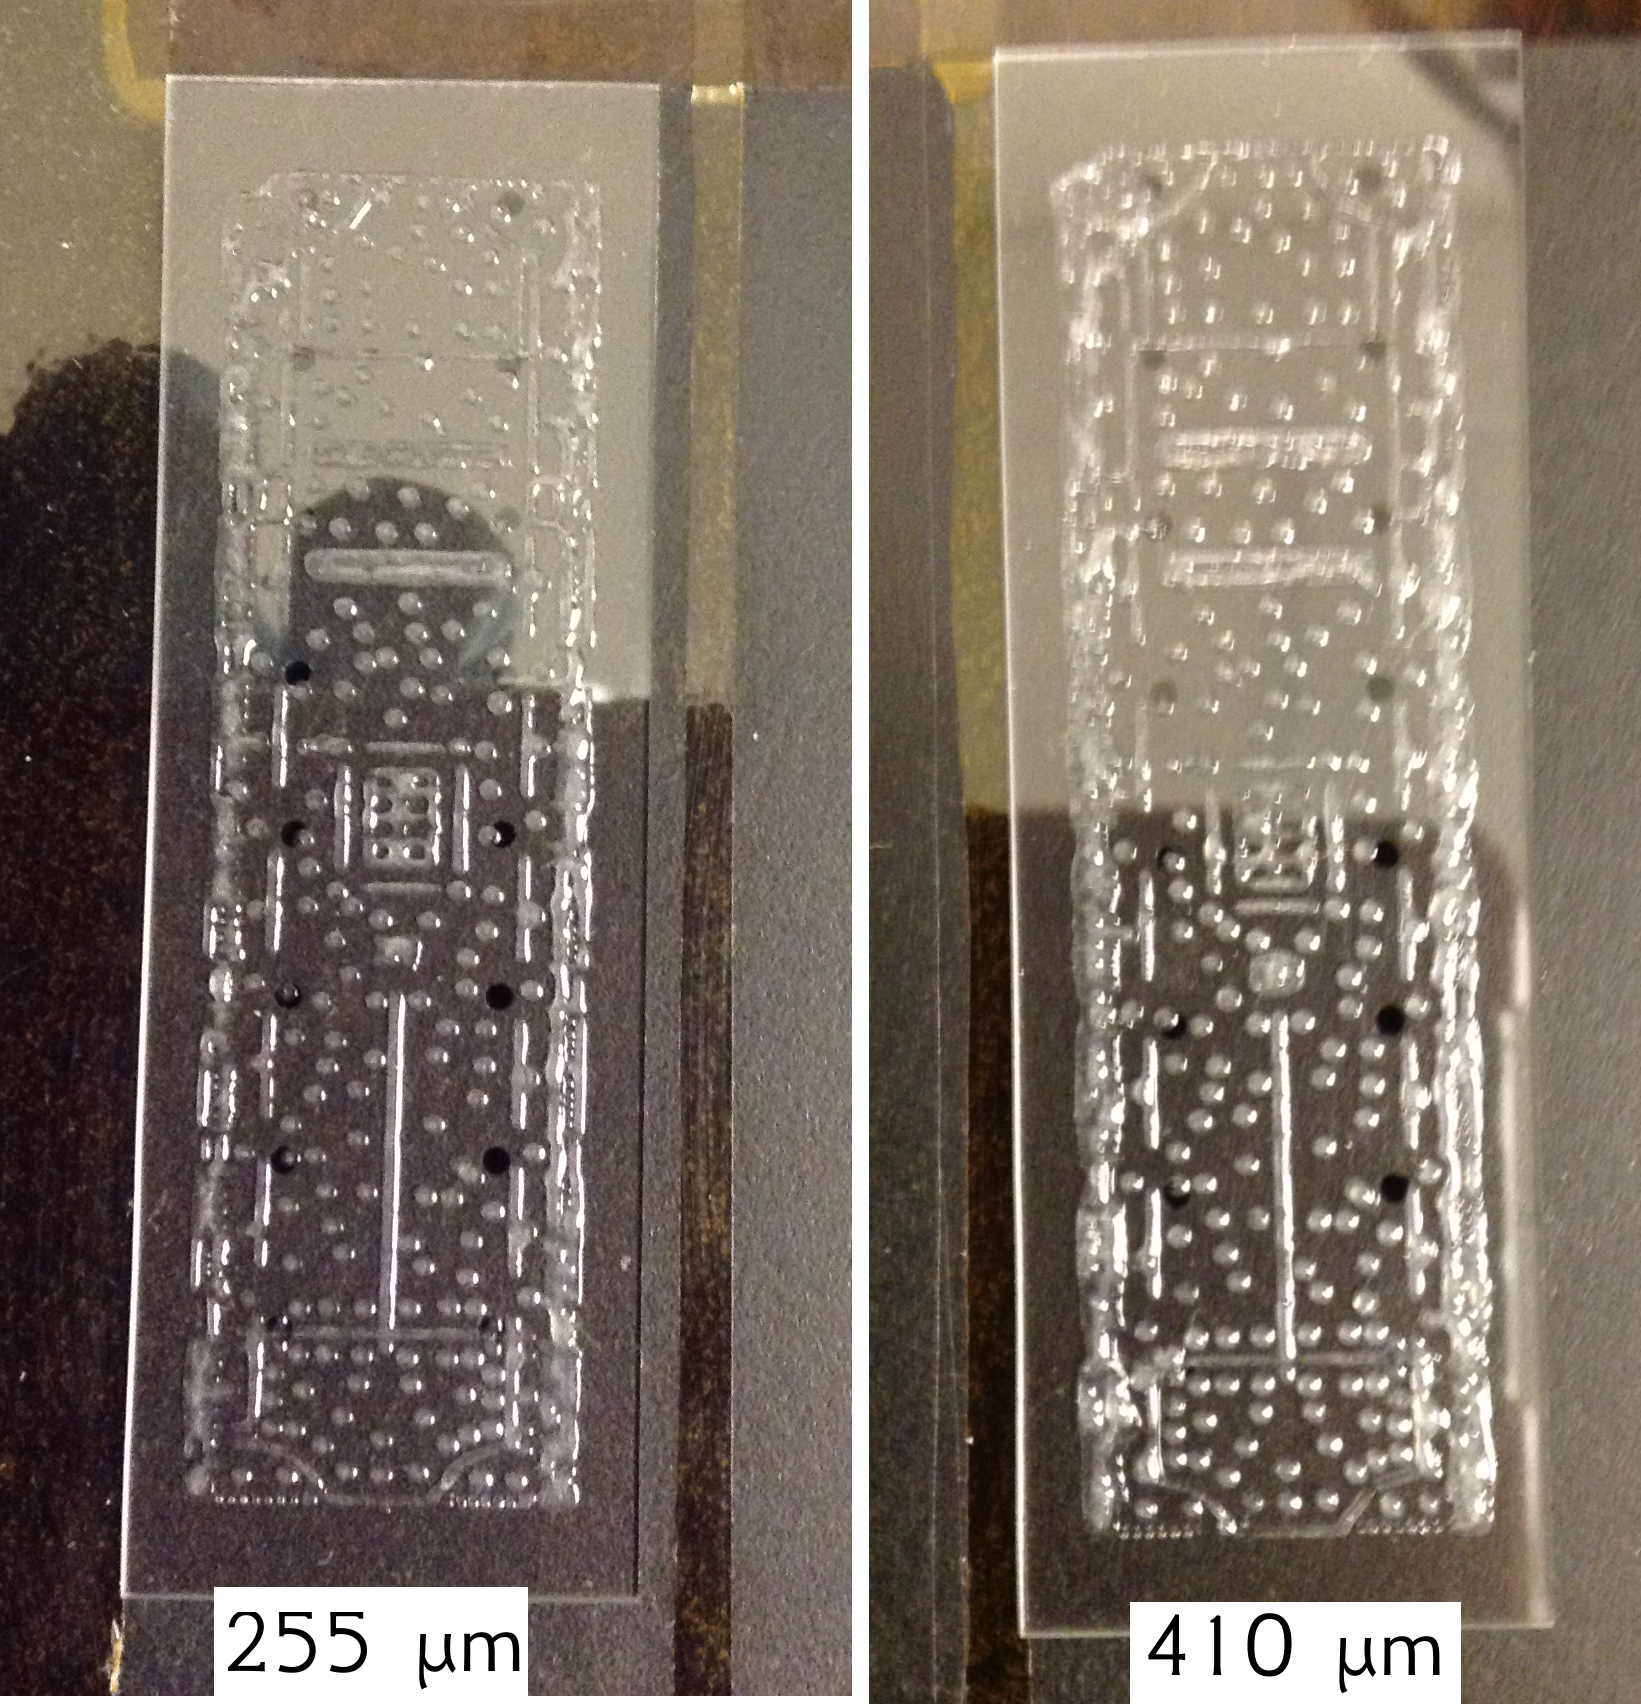
\includegraphics[width=0.4\textwidth, height=0.4\textwidth]{pixel/glue_test_depth2}\\
  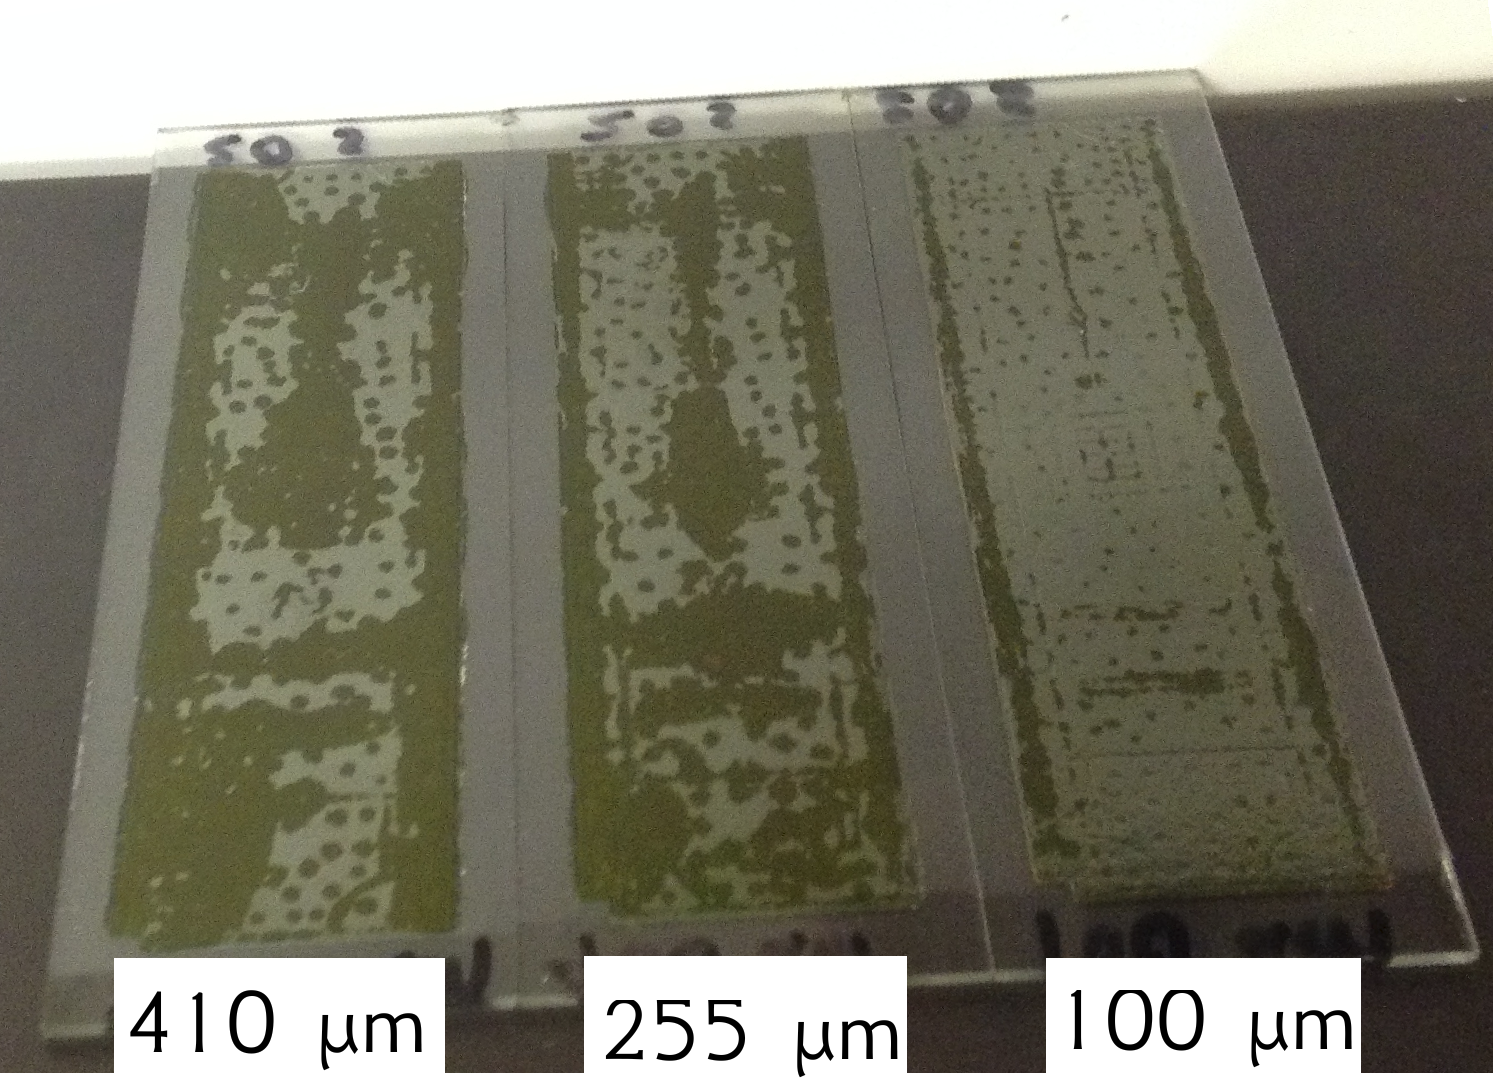
\includegraphics[width=0.6\textwidth]{pixel/glue_test_depth1}
  \caption[Test of amount of glue deposited.]{Pictures of a test of the amount of glue dispensed as a function of the glue reservoir depth. The glue reservoir depth was varied by adding kapton tape (left), and the test were conducted by gluing plain HDI on top of glass slides (middle and right.)}\label{fig:glue_test_depth}
\end{figure}

\item \ti{the amount of glue dispensed}, and in particular the glue spreading out of the HDI area. An excess of glue, scattered beyond the HDI edge would go between the ROC and the sensor, affecting the functionality of the bump bonds connecting them; in the case of the high voltage (HV) pad, it was observed that the excess of glue covers the pad on the sensor, making impossible to wire it. The amount of glue deposited on  top of BBM depends on several variables: the dipping time of the stamp tool in the glue reservoir, the time that the stamp tool is in contact with the BBM, and the depth of the glue reservoir. In the case of the dipping and stamping times, it was found that there is not a strong dependence and those times were set to 10 seconds; in the case of the glue reservoir depth, the dependence is stronger. Several glue tests where conducted by gluing plain HDIs to glass slides; Figure~\ref{fig:glue_test_depth} shows pictures from a glue test with three different glue reservoir depths (100 $\mu$m, 255 $\mu$m and 410 $\mu$m). The results show not only that the deeper is the glue reservoir the bigger is the amount of glue deposited, as expected, but also that the spreading out is critical for the depths greater than 200 $\mu$m. A redesign of the rubber stamp pattern was made in order to reduce the amount of glue deposited in the HDI pads regions; that adjustment led to the final rubber stamp pattern.

\begin{figure}[!h]
  \centering  
  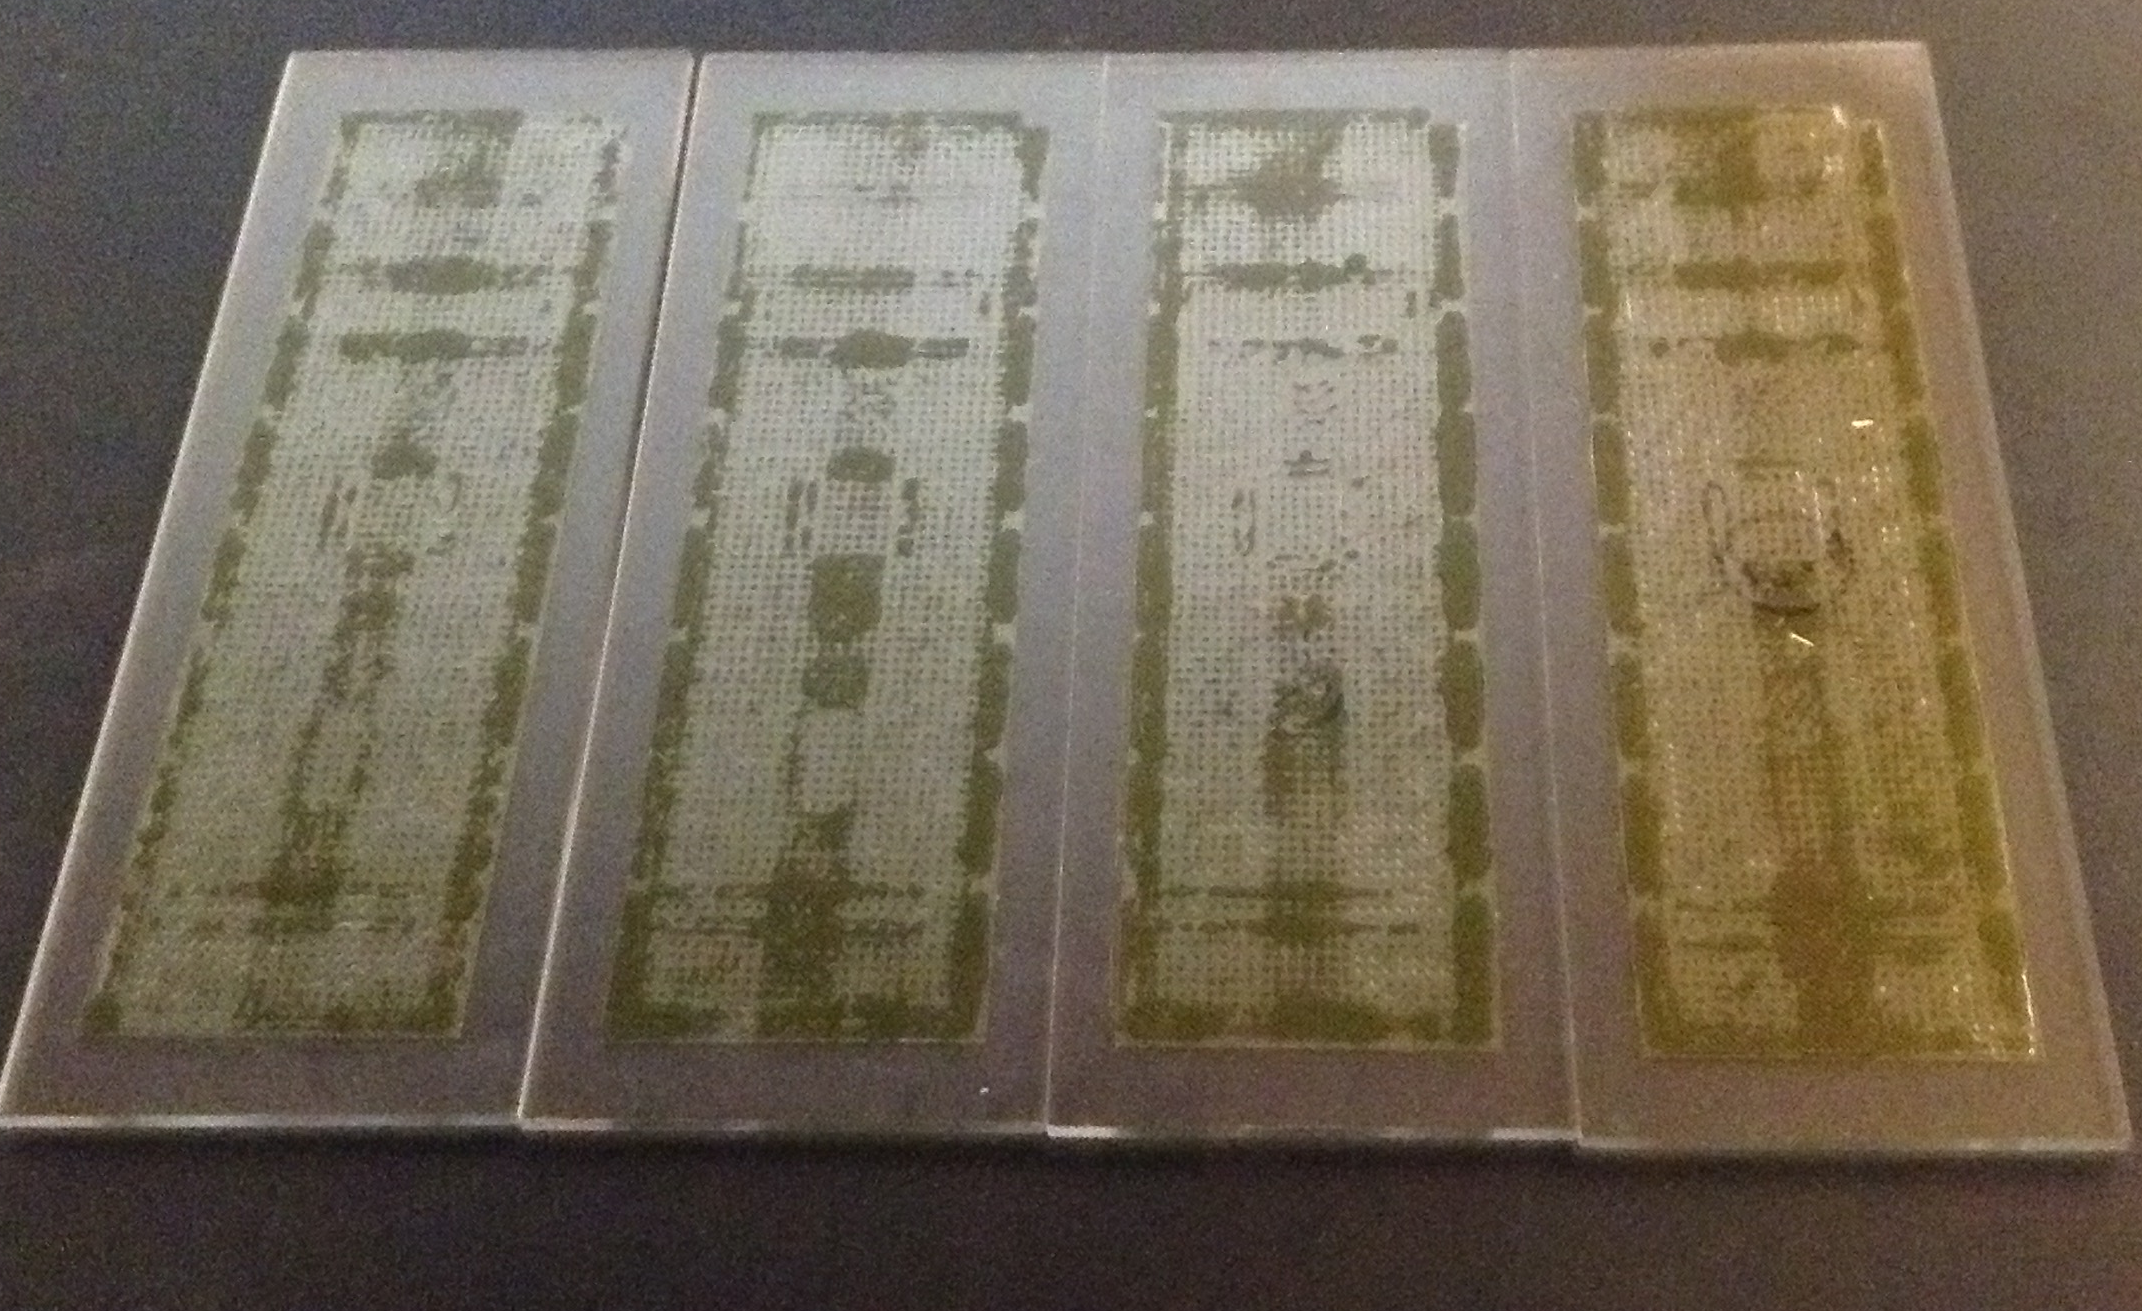
\includegraphics[width=0.6\textwidth]{pixel/glue_test_contact1}\\
  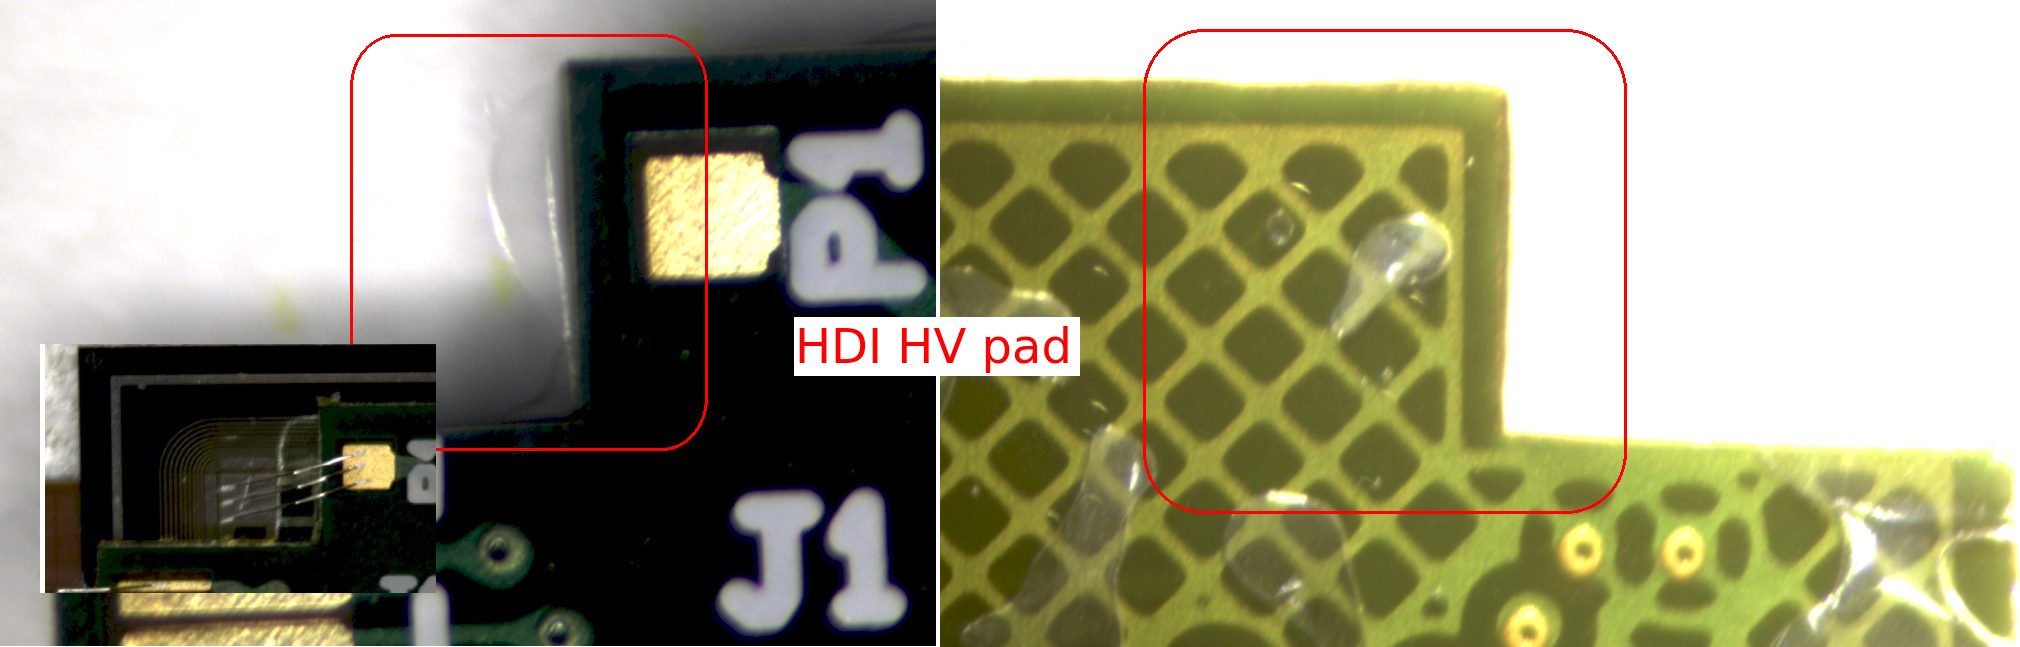
\includegraphics[width=0.8\textwidth]{pixel/hd_pad1}
  \caption[Glue contact area test.]{Results from a glue test using the final stamp pattern, which proves the support provided to the HDI bond pads and the HV pad and the almost null glue spreading out.}\label{fig:glue_test}
\end{figure}

\item \ti{the size of contact area}, and in particular the support given to the edges of the HDI where the bond pads and the HV pad are located. This is a critical aspect, given that the wirebonding relies on the steadiness of the pads to be connected. Figure~\ref{fig:glue_test} shows the outcomes of a glue test using the final stamp pattern; note the support provided to the HDI bond pads and the HV pad and the almost null glue spreading out, it justifies why this stamp pattern was chosen.   
\eit

The final tools designs used during the module production are indicated in Figures \ref{fig:st_wt} and \ref{fig:stamp_pattern}, while the optimal glue reservoir depth was found to be 100 $\mu$m. 

\subsubsection*{Grabber and picker tools}

\begin{figure}[!h]
  \centering  
  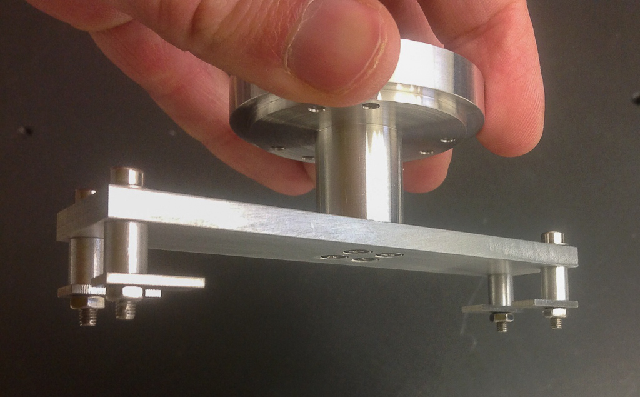
\includegraphics[width=0.60\textwidth,height=0.33\textwidth]{pixel/grabber}\\
  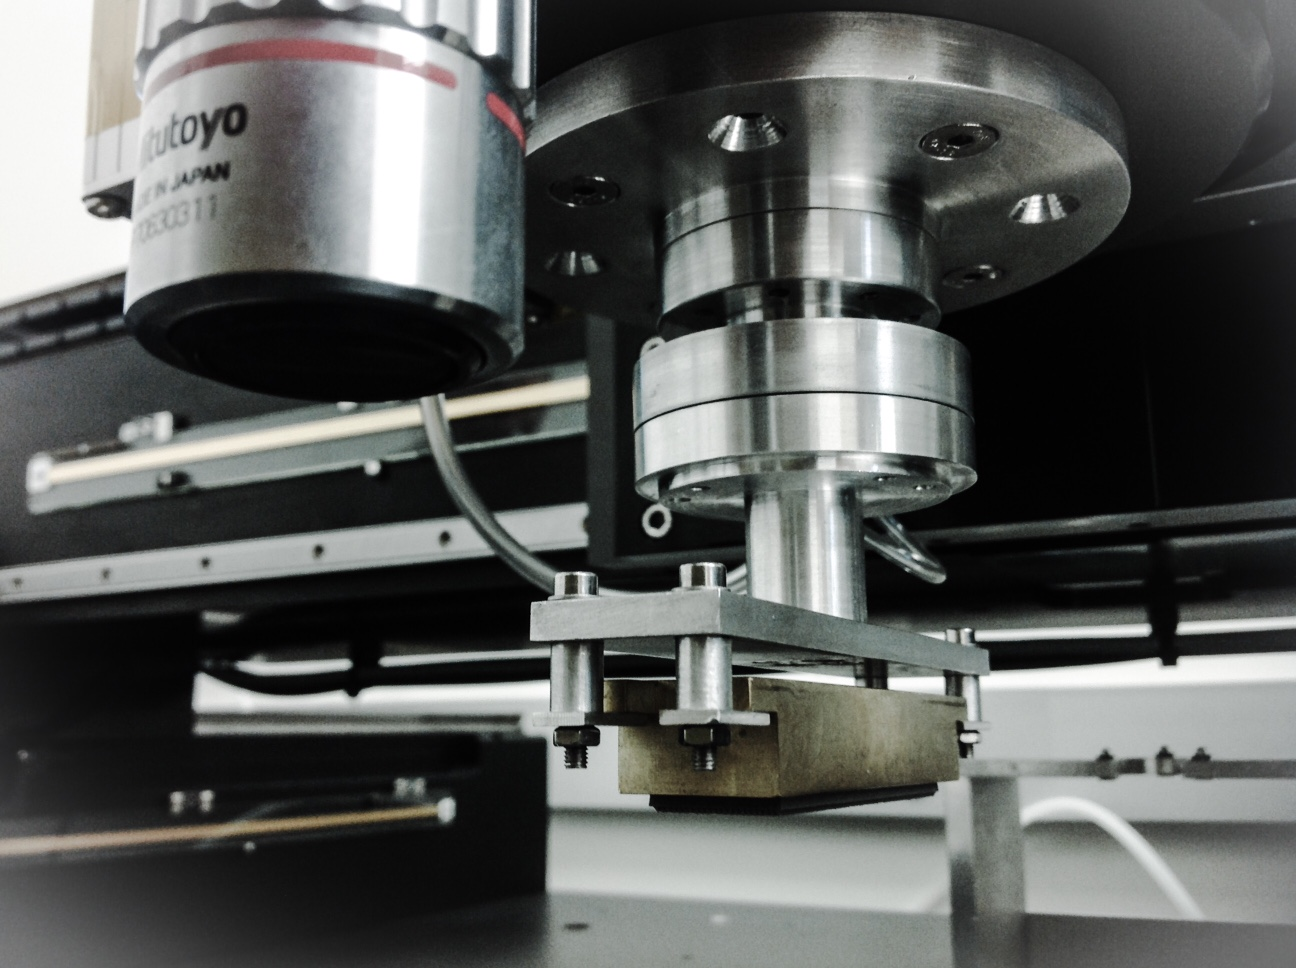
\includegraphics[width=0.45\textwidth,height=0.33\textwidth]{pixel/GrabberToolHoldingStamp}
  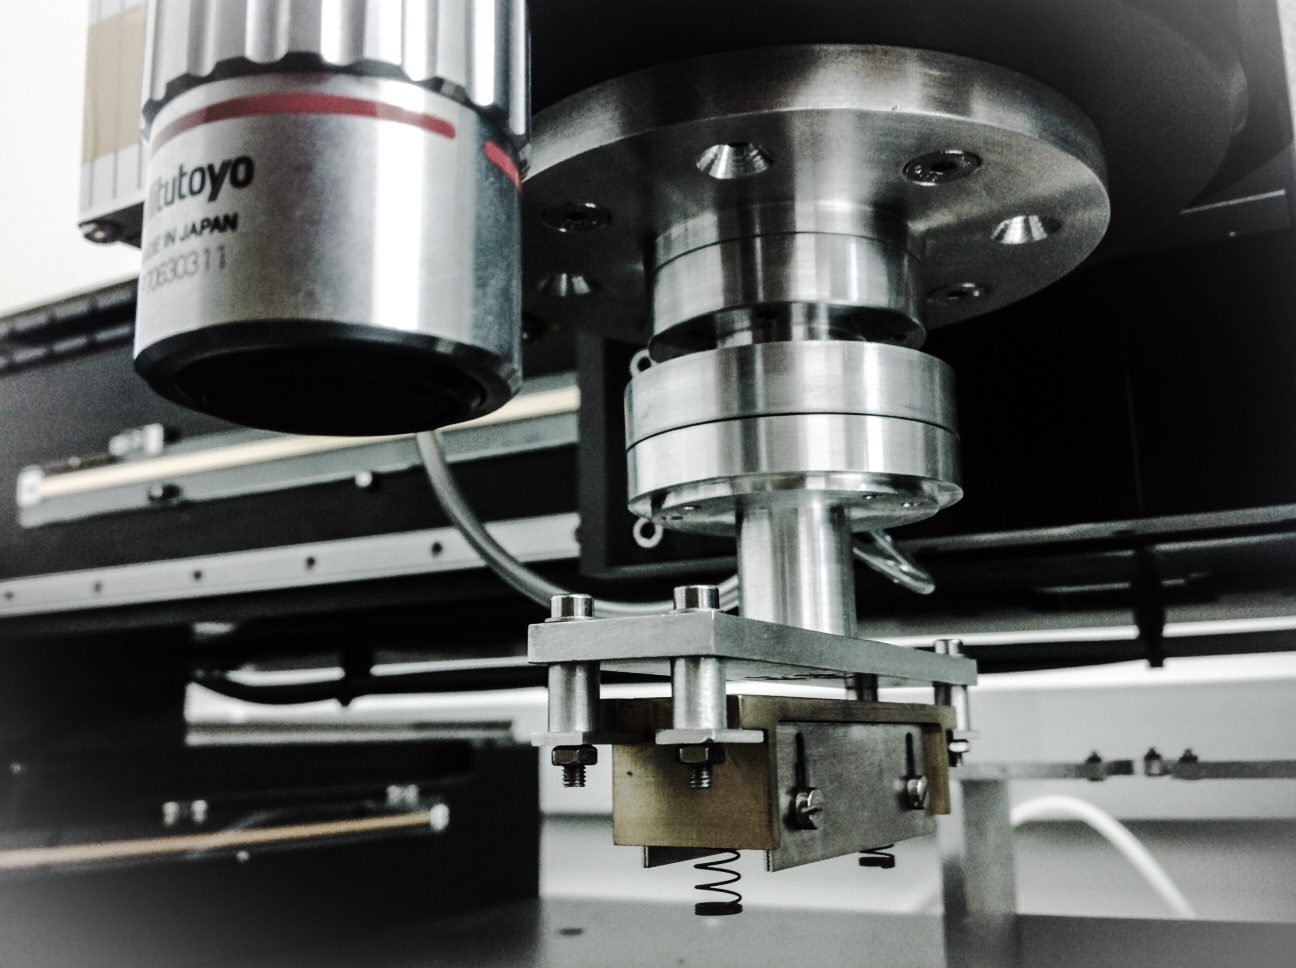
\includegraphics[width=0.45\textwidth,height=0.33\textwidth]{pixel/GrabberToolHoldingWeight}
  \caption[Grabber tool.]{Top: Grabber tool used to grab the stamp and weight tools from their houses to the BBM location. Bottom: grabber tool holding the stamp (left) and weight (right) tools.}\label{fig:grabber_tool}
\end{figure}

In order to move the stamp and weight tools from their houses to the glue reservoir and to the BBM location, a \ti{grabber tool} was designed. The grabber tool is held on a tool rack located in the back of the gantry table and it gets attached to the gantry head by using an adapter and the vacuum system as shown in Figure\ref{fig:grabber_tool}. The gantry head adapter is attached to the rotary motor that provides the angular motion, therefore, the grabber tool is able to grab the stamp and weight tools and adjust their alignment in agreement with the BBM orientation. The force with which the glue is applied on the BBM is controlled by the weight of the brass piece; in a similar way, the force applied to the HDI-BBM sandwich is controlled by the weight of the tool and the springs.                  

The pick of the HDI and place on top of the BBM is performed using the \ti{Picker tool} showed in Figure \ref{fig:pandp_tool}. Same as the grabber tool, the picker tool is held at the tool rack until the gantry head goes to its location and catches it using vacuum; an independent vacuum line is used to capture the HDI from its chuck slot. The alignment is performed while the HDI is being moved to the BBM location.      
\begin{figure}[!h]
  \centering  
  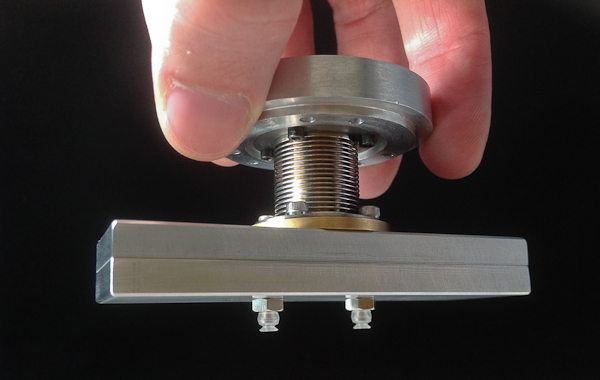
\includegraphics[width=0.45\textwidth,height=0.3\textwidth]{pixel/pickNplace}
  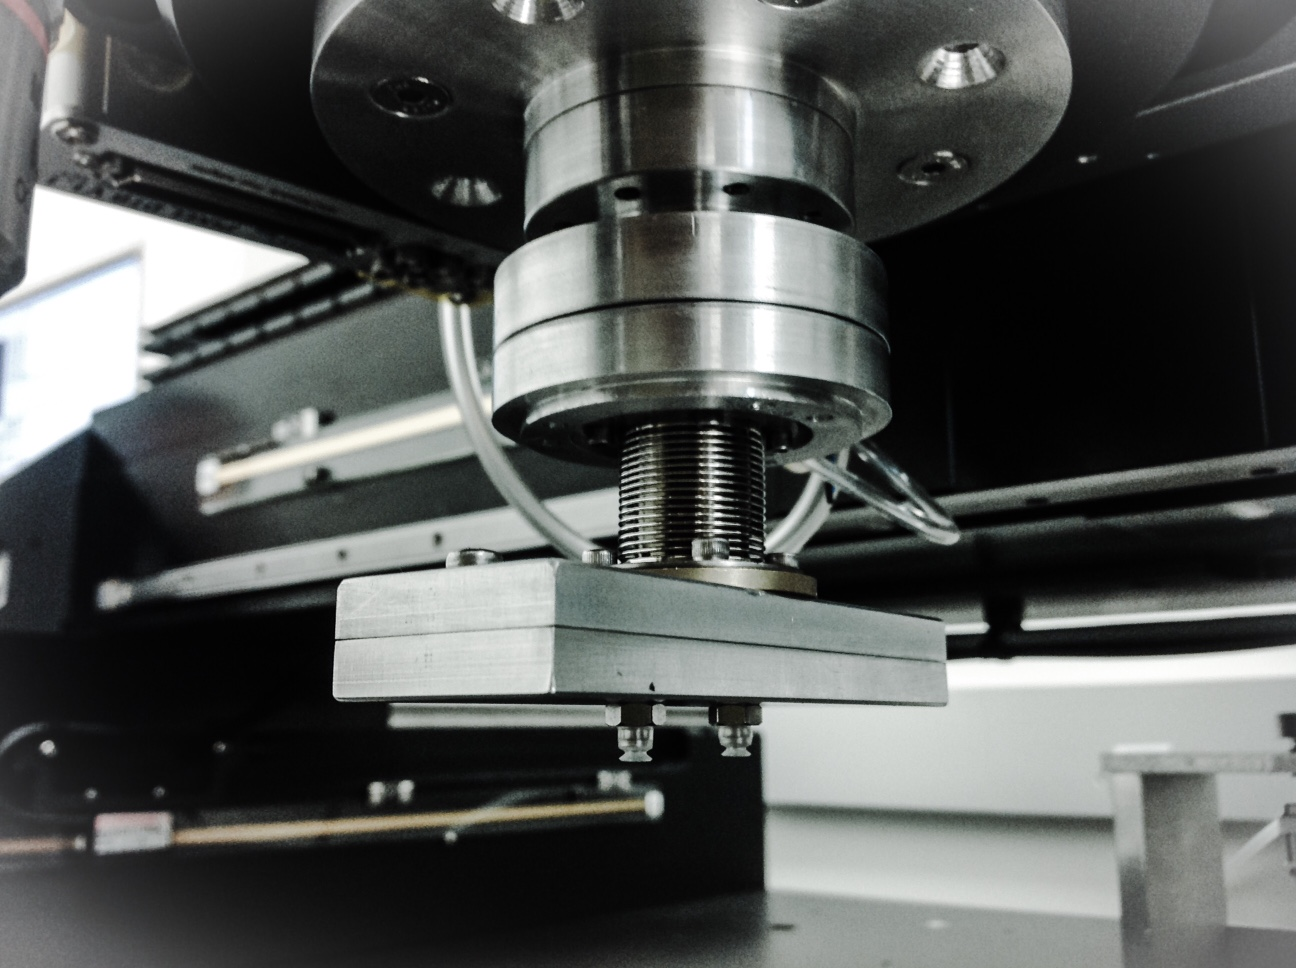
\includegraphics[width=0.45\textwidth,height=0.3\textwidth]{pixel/PickAndPlaceTool}
  \caption[Pick and place tool.]{The pick and place tool, picks the HDI from its chuck and place it on top of the BBM.}\label{fig:pandp_tool}
\end{figure}

\subsubsection*{Vision system}

A vision hardware system, attached to the gantry head, is used to locate the module components and tools employed in the assembly process. It is composed of a IDS HD digital camera and a Mitutoyo wide-field video microscope unit (WIDE VMU) as shown in Figure \ref{fig:setup}. The vision hardware is complemented with auto-focus and pattern recognition algorithms. 

\begin{figure}[!h]
  \centering  
  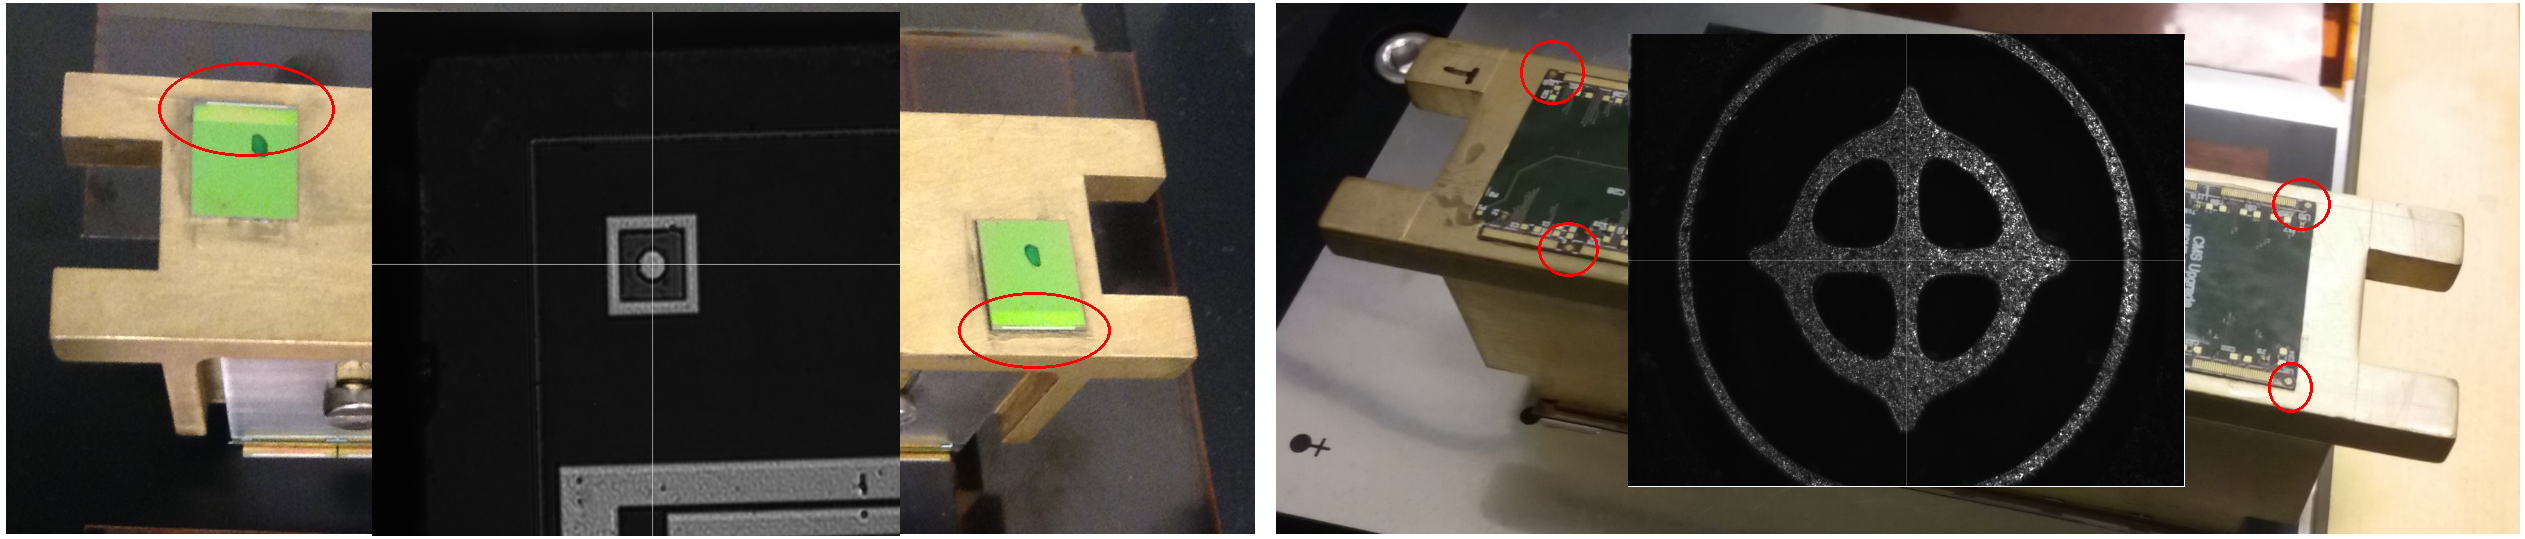
\includegraphics[width=\textwidth]{pixel/fiducial_tools}\\
  \caption[Fiducial marks on tools.]{Fiducial marks attached to the stamp and weight tools. Initially, non-functional ROCs were glued on top of the tools (left) to provide the fiducial marks, which were located in the places indicated by red circles; later they were replaced by plane HDIs (right).}\label{fig:fiducial_tools}
\end{figure}

Given that the coarse location of the HDIs, BBMs, stamp and weight tools are well defined by the location of the stencils and plates on the gantry table, the vision system is designed to search and find fiducial marks present on the materials and tools; these fiducial marks are placed on the HDI and BBM during their fabrication process. In the case of the tools, two methods were used to attach a fiducial mark to them: non-functional ROCs, which have on themselves fiducial marks, were glued on top of the tools as shown in Figure \ref{fig:fiducial_tools}, however, during the gluing and cleaning processes the fiducial marks were usually covered with glue remainders or broken, making necessary their replacement very often; the second method consisted of gluing plane HDIs on top of the tools, which not only solved the issues with the destruction of the fiducial marks but also simplified the pattern recognition.

The procedure to find the fiducial marks starts by moving the camera to an initial default calibrated position above the element, HDI, BBM or tool, such that the image in the field of view of the camera contains the fiducial mark; then, the auto-focus algorithm finds the best focus by measuring the contrast of pictures taken by the camera at ten different positions in $z$ direction around a default position where it is assumed the best focus is; these ten contrasts are then fitted to a Gaussian distribution where the maximum of the fitting corresponds to the best focus.     

Once the best focus is found, the gantry head moves the camera to that position, takes a new picture and send it to feed the pattern recognition algorithm which use k-means clustering to separate the foreground from the background; then, the foreground (Fiducial + noise) is dilated to close any small holes in the image and to extract contours from the image.

\begin{figure}[!ht]
  \centering  
  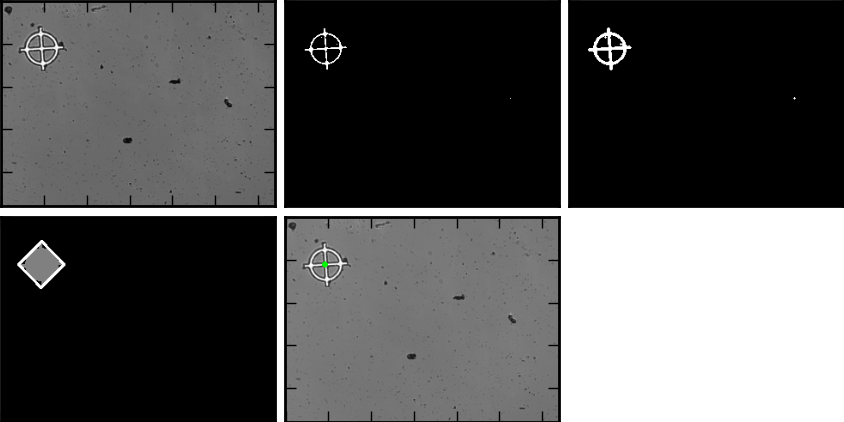
\includegraphics[width=0.8\textwidth]{pixel/BBM_fid1.png}
  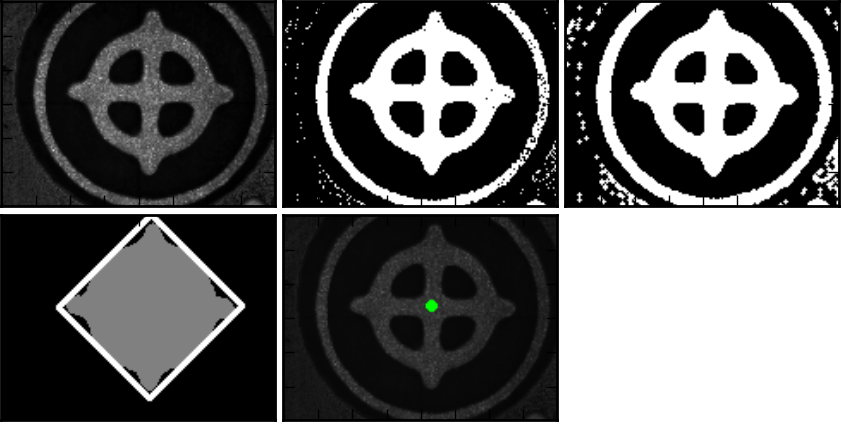
\includegraphics[width=0.8\textwidth]{pixel/HDI_fid1.png}
  \caption[Fiducial mark recognition.]{Fiducial mark recognition: BBM (two top rows) and HDI (two bottom rows). The input image is processed to define contours; after filtering, the centroid of the recognized fiducial mark is returned by the algorithm and indicated in the input image by the green dot.}\label{fig:BBM_fid1}
\end{figure}

The fiducial mark features are parametrized in terms of its size and aspect ratio with respect to the field of view of the camera, therefore, by filtering the contours on size and aspect ratio it is assured that one and only one contour passes filters. Later, the algorithm calculates the minimum bounding box and centroid of the fiducial mark to finally return the centroid as fiducial mark center and the distance between centroid and box center as a measure of goodness. In order to reduce the processing time, the input image resolution is reduced by a factor of 8. The algorithm was written by Caleb Fangmeier and is documented in Reference \cite{pr_algorithm} from where Figure \ref{fig:BBM_fid1} was taken.

\subsubsection*{Gantry head center-camera offset (GHCO)}

The \ti{global coordinate system} of the setup is centered in the so-called \ti{home position} located in the back-left side of the gantry table; thus, the origin of the coordinate system is defined by the position of the gantry head center when it is placed at home position. Any distance is then measured by comparing the gantry head center position at a given location and the home position. While the tool adapter is concentric to the gantry head (and then its coordinates are the same as the gantry), the camera has an offset with respect to the origin of the global coordinate system because the vision system is not located at the gantry head center, therefore, any location provided by the vision system has to be corrected by this offset, known as \ti{Gantry head center-camera offset} (GHCO).

\begin{figure}[h]
\begin{center}
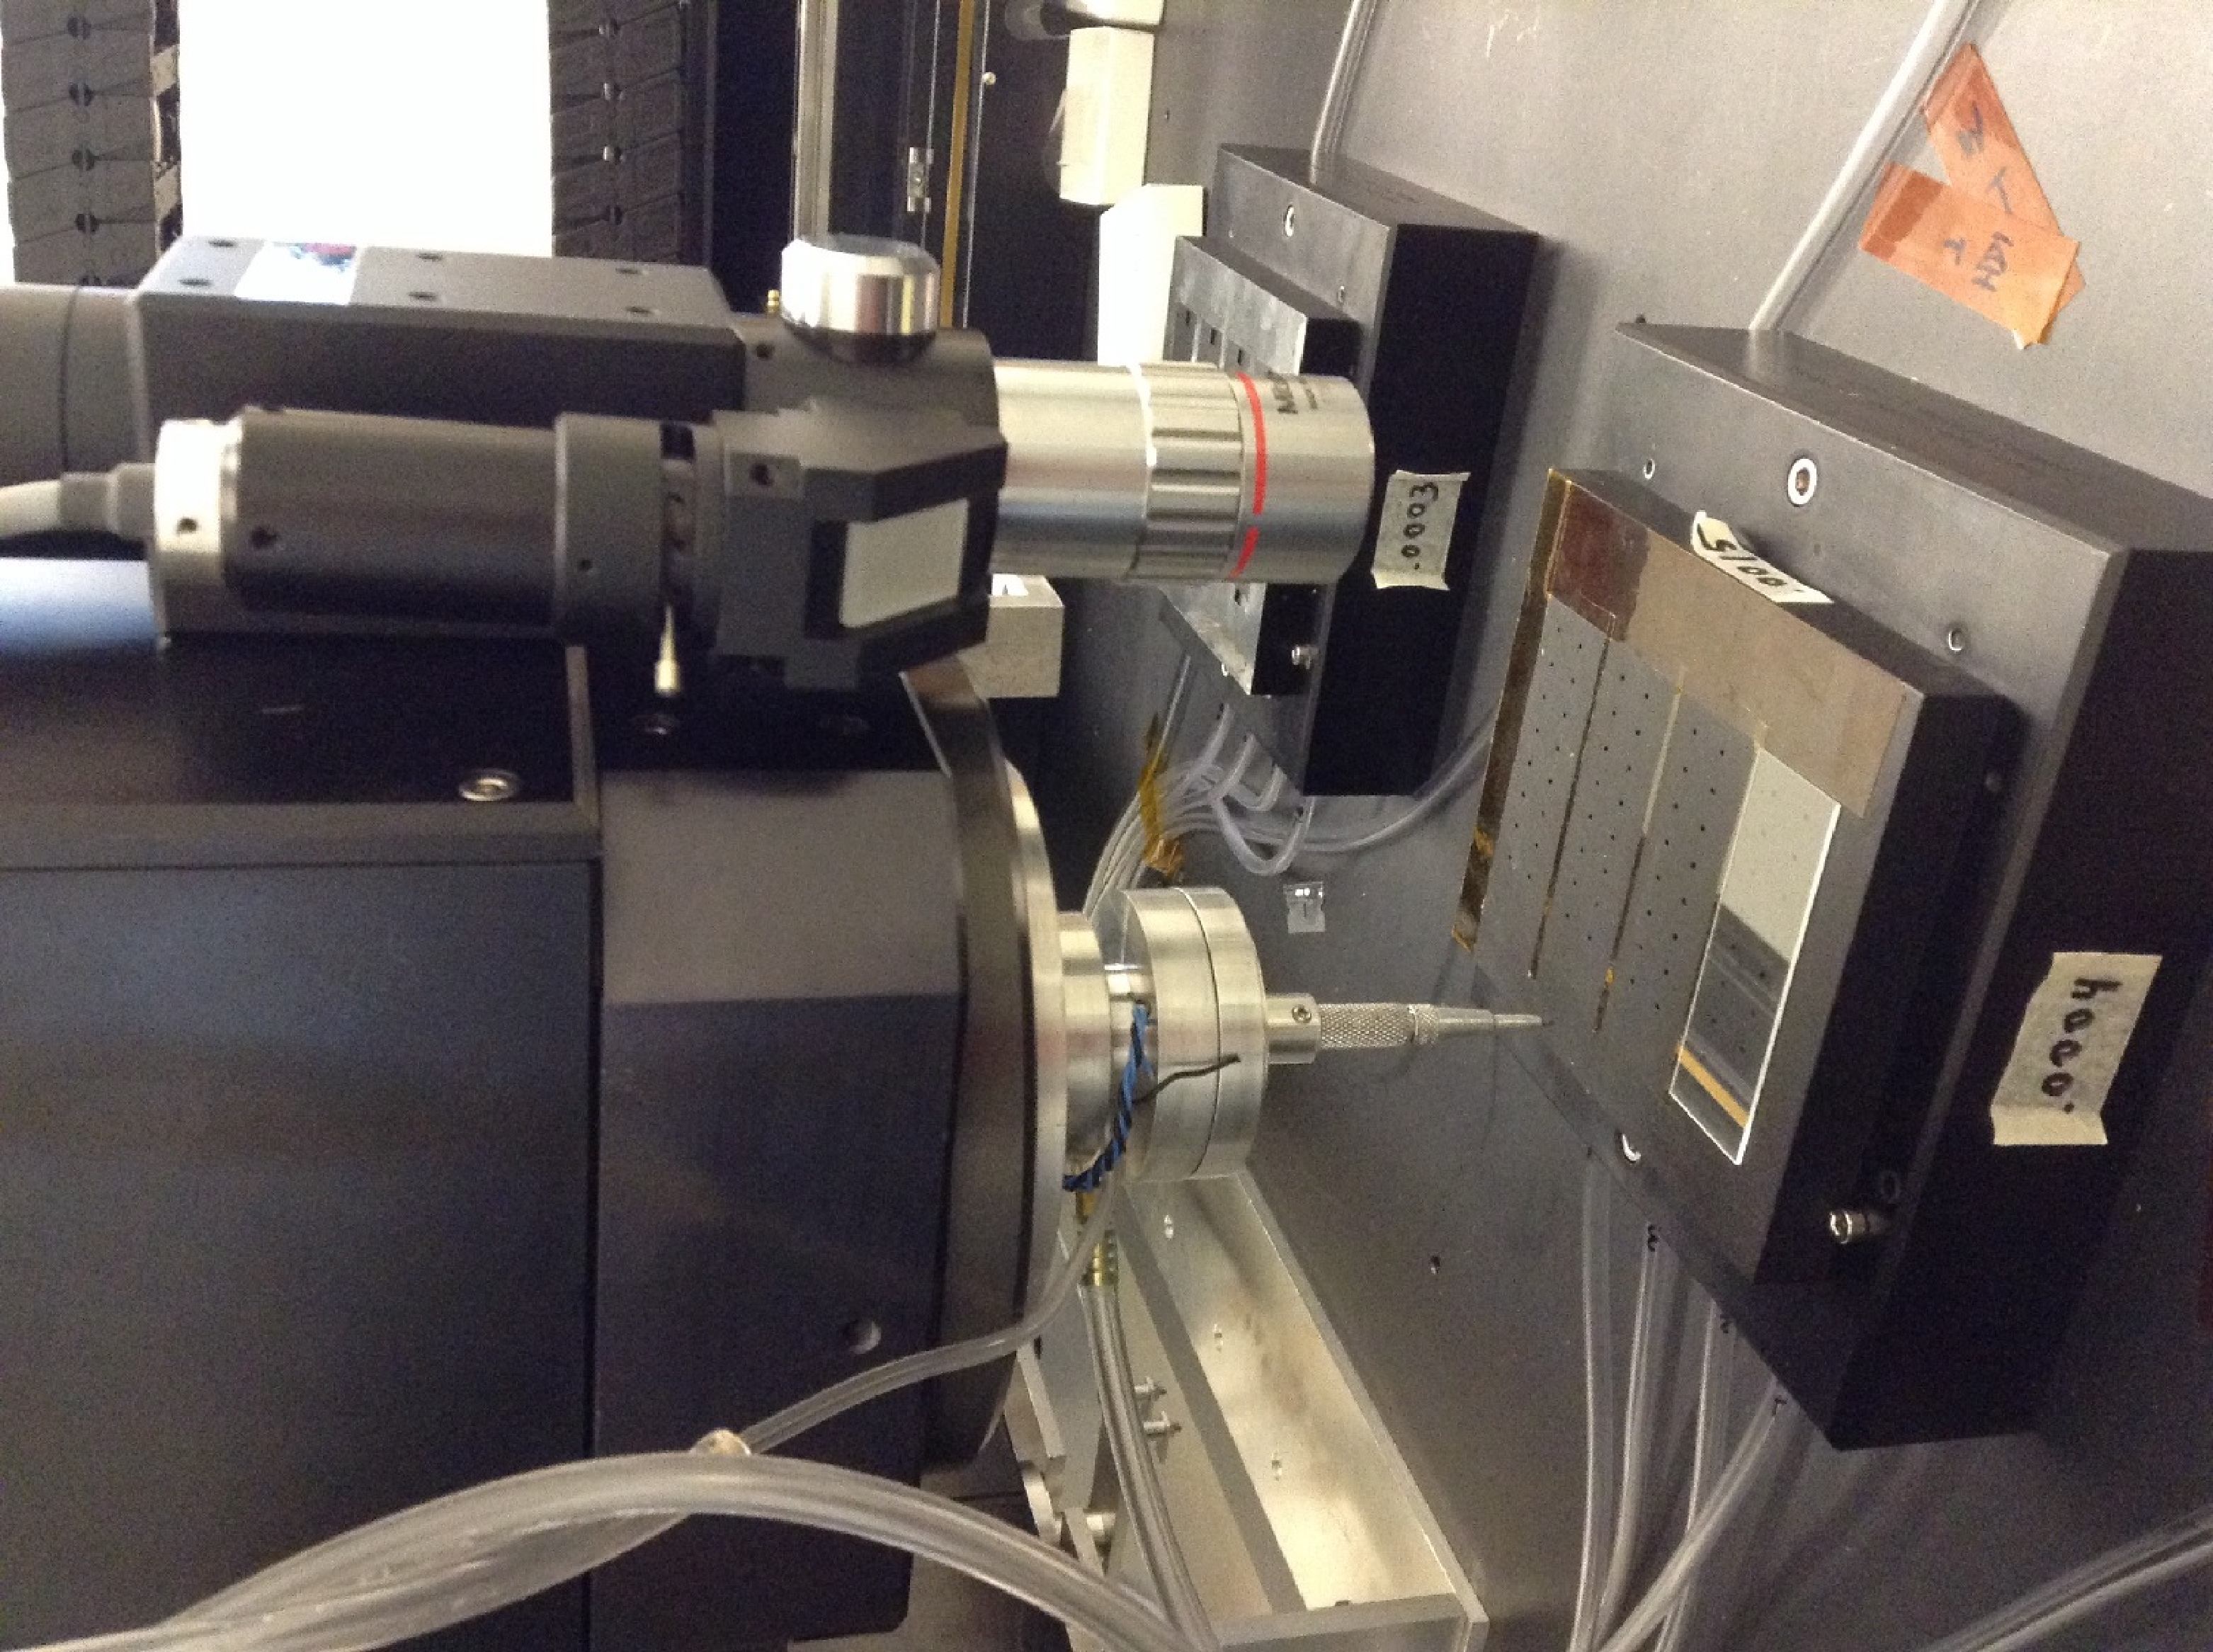
\includegraphics[width=0.45\textwidth,angle=-90]{pixel/offset_setup}
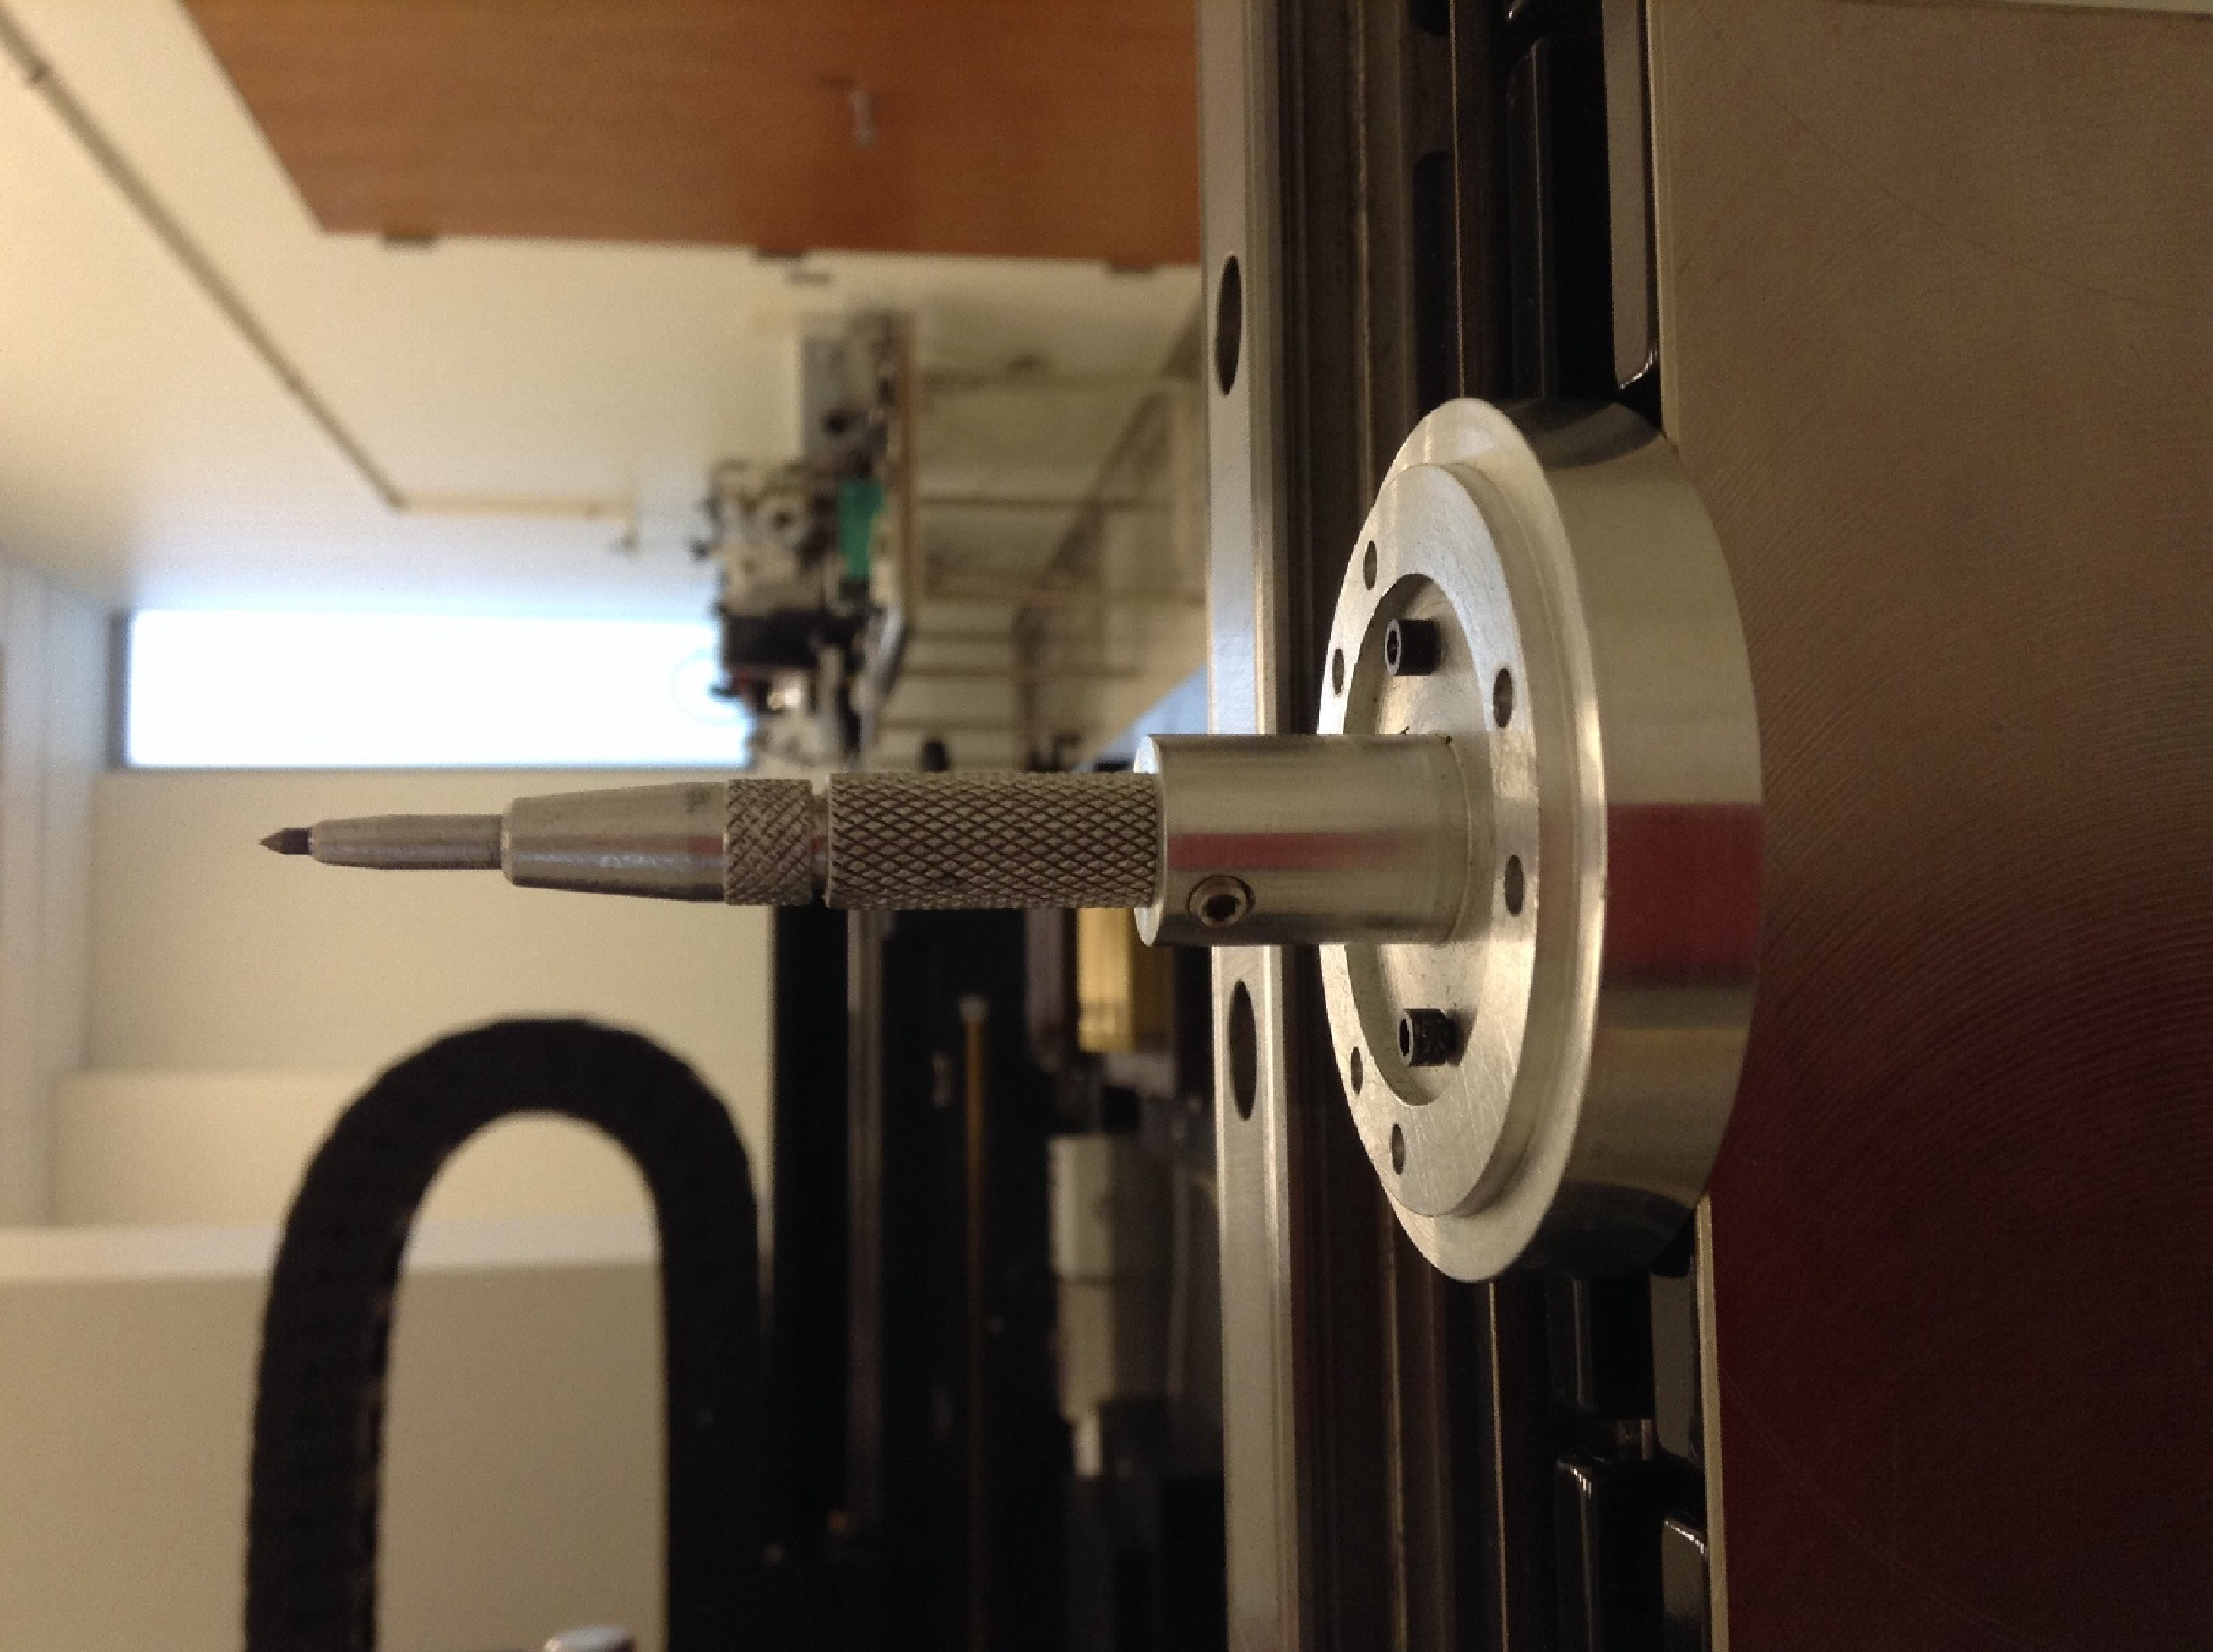
\includegraphics[width=0.45\textwidth,angle=-90]{pixel/scratch_tool}
\caption{Setup used to measure the GHCO}\label{fig:offset_setup}
\end{center}
\end{figure}

To determine the GHCO, a set of 40 marks (scratches) were made on a glass slide using a needle shaped tool with the tip made of carbide (see Figure \ref{fig:offset_setup}); the locations of the scratches were predefined and known as commanded positions. Later, the camera was moved to find the scratches and their locations were tagged as observed positions. In principle, the difference between the commanded and the observed positions provide a measurement of the GHCO, but it cannot be assumed that the needle tool is straight, i.e., if the tip of the tool coincides with the gantry head center; in order to take into account this fact when calculating the offset, a scratching scheme was designed; it is showed in Figure \ref{tool_bend}. In the ideal case, the scratch is made right in the commanded position (red circle), but if the needle is not straight, the scratch will be shifted (black cross). A rotation of the tool can be used to determine how bend is the needle tip.

\begin{figure}[h]
\begin{center}
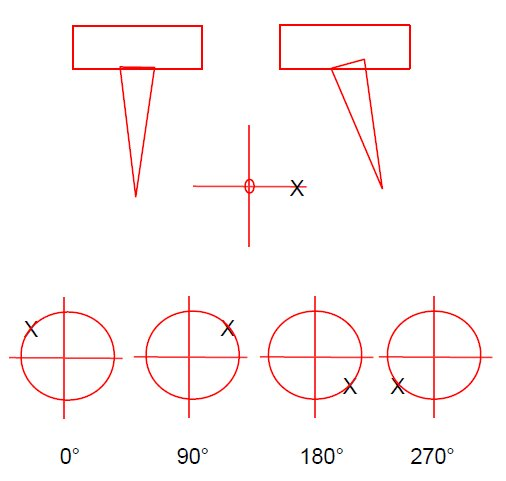
\includegraphics[width=0.7\textwidth]{pixel/tool_bend}
\caption{Scratches scheme if the tool is not straight }\label{tool_bend}
\end{center}
\end{figure}

A precise procedure for measuring the GHCO is performed by a labVIEW program (\ti{offset\_fitting.vi}) which implements the following steps 

\begin{itemize}
\item pick the needle tool from the tool rack,
\item move the gantry to the first scratch position (the commanded position),
\item make the scratch moving the tool down.
\item move the tool back up
\item move the gantry to the next scratch commanded position.
\item Repeat the process to make nine more scratches.
\item Rotate the tool by $\theta=90^o$ and repeat the process to make ten new scratches.
\item Rotate the tool by additional $90^o$ (now the total rotation is $\theta=180^o$) and make ten more scratches.
\item Rotate the tool by additional $90^o$ (now the total rotation is $\theta=270^o$) and make ten more scratches.
\item Move the camera to the first scratch position and locate the center of the scratch, capture the position.
\item Repeat the process to locate the rest of the scratches.   
\end{itemize}

The operator only interacts with the program by capturing the positions. The output of the program is a text file that contains all the commanded and observed positions. The set of measurements are statistically treated, using the linear least squares fitting technique. The model describing the location of the scratches system is parametrized by a linear combination of a set of functions weighted by a set of parameters;

\begin{equation}
y(x)= f(y,\textbf{a})=a_1f_1(x)+a_2f_2(x)+.....+a_pf_p(x)
\end{equation}

The residuals, which correspond to the difference between the predicted value from model ($f(x_i, \textbf{a})$) and the measured value $y_i$, are calculated using 

\begin{equation}
r_i= y_i - f(x_i\textbf{a}),
\end{equation}

\noindent one wants to minimize these residuals and more specifically their squares (S). The fit will provide the values of the parameters $\textbf{a}$, so that the model is totally defined. In matrix form, for a set of measurements $(x,y)$ :

\begin{equation}
\textbf{Y}= A \textbf{a}
\end{equation}
\begin{equation}
S=\textbf{r}^T\textbf{r}
\end{equation}

The matrix A encloses the features of the system/model, the vector \textbf{a} encloses the parameters under evaluation and the vector \textbf{Y} encloses the taken measurements and the predictions made by the model. After the minimization, the vector of parameters can be written as:

\begin{equation}\label{solution}
\textbf{a}=(A^TV^{-1}A)^{-1}A^TV^{-1}\textbf{Y}
\end{equation}

\noindent where V is the covariance matrix; it contains the information about the correlation among measurements and the uncertainty of the measurements.

\begin{equation}
  V=
  \begin{pmatrix}
    \sigma_1^2  & \sigma_{12}  & \cdots & \sigma_{1n} \\
    \sigma_{21} & \sigma_2^2   & \cdots & \sigma_{2n} \\
    \vdots      & \vdots       & \ddots & \vdots      \\
    \sigma_{n1} & \sigma_{n2}  & \cdots & \sigma_n^2
  \end{pmatrix}
\end{equation}

The model for one measurement $(x,y)$, \ie, only one scratch, can be written as:

\begin{equation}
\begin{pmatrix}
x\\ 
y
\end{pmatrix}-
\begin{pmatrix}
x_g\\ 
y_g
\end{pmatrix}=
\begin{pmatrix}
\Delta x_{GHCO}\\ 
\Delta y_{GHCO}
\end{pmatrix}
+
\begin{pmatrix}
c  & s\\ 
-s & c
\end{pmatrix}
\begin{pmatrix}
c' & s' \\ 
-s'& c' 
\end{pmatrix}
\begin{pmatrix}
1\\ 
0
\end{pmatrix}
\end{equation}


\noindent where, ($x_g,y_g$) are the commanded positions, $(\Delta x_{GHCO},\Delta y_{GHCO})$ are the offset components in $x,y$ directions respectively, $c=r\cos\phi$ and  $s=r\sin\phi$ describe the bending of the needle tool in terms of the radius $r$ of the circle and the angle $\phi$ (see Figure \ref{tool_bend}); $c'=\cos\theta$ and  $s=\sin\theta$ describe the rotations of the tool ($\theta=0^o, 90^o, 180^o, 270^o$) with respect to the $x$ direction.

The matrix A and the vector of parameter \textbf{a} can be written as:

\begin{equation}
  A=
  \begin{pmatrix}
    1  & 0  & c' & -s' \\
    0  & 1  & -s' & -c' 
  \end{pmatrix}, \quad
  \textbf{a}=
  \begin{pmatrix}
    \Delta x_{GHCO}\\ 
    \Delta y_{GHCO}\\
    c \\
    s 
  \end{pmatrix}
\end{equation}

The matrix A, including the full set of forty pairs of measurements ($x,y$), is a $4\times80$ matrix where in the first ten rows $c'=\cos(\theta=0)=1, s'=\sin(\theta=0)=0$, while in the second ten rows $c'=\cos(\theta=90)=0, s'=\sin(\theta=90)=1$ and so on.   

The offset\_fitting.vi program integrates a Matlab script that solves the matrix equation \ref{solution}, using the commanded and observed positions measured by the vision system; the uncertainties were assumed to be the same for all measurements and additionally it was assumed that the measurements are not correlated, so the covariance matrix is the uncertainty ($\sigma=0.01 \mu$m) times the $80\times80$ identity matrix. The results for the GHCO and the radius are:

\begin{align}
  \Delta x_{GHCO}=& 0.482 \pm 0.008 mm\nonumber\\
  \Delta y_{GHCO}=& -102.362 \pm 0.008 mm\\
  r=&0.042 \pm 0.007 mm\nonumber.
\end{align}

\subsubsection*{The dispensing system}

The dispensing system components are shown in Figure \ref{fig:potting_comp}. The dispenser and syringe holder are attached to the gantry head as shown in Figure \ref{fig:setup}. The encapsulant is a mixture of sylgard curing agent and sylgard base elastomer in a proportion 1:10; the volumes are measured using common syringes, and the mixing is performed on a plastic sheet. Several needle tip sizes were tested in order to optimize the amount of sylgard dispensed in agreement with the pressure provided by the dispenser; the needle chosen has an internal diameter of 150 $\mu$m.

\begin{figure}[h]
  \begin{center}
    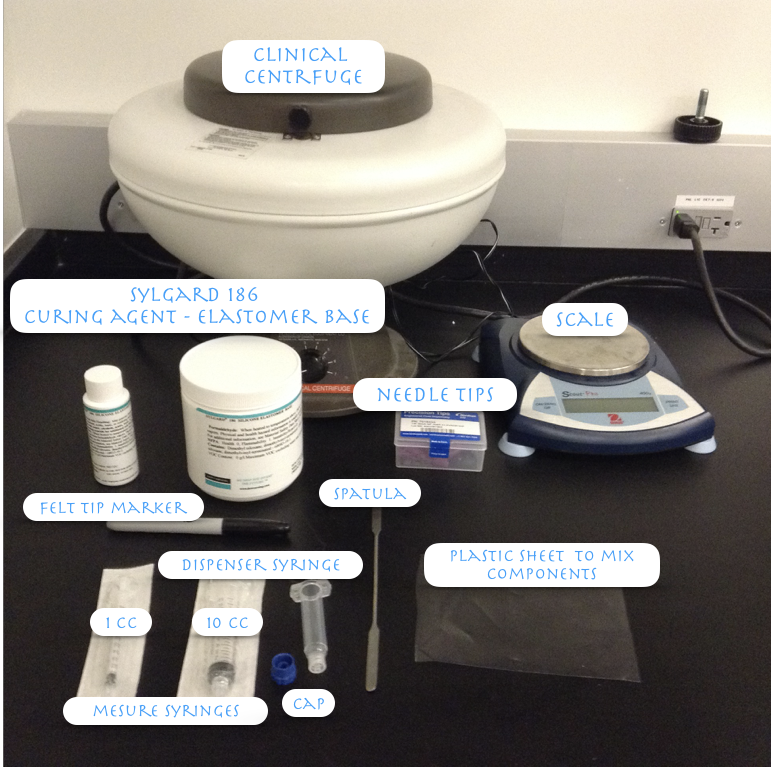
\includegraphics[width=0.45\textwidth,height=0.55\textwidth]{pixel/materials_potting}
    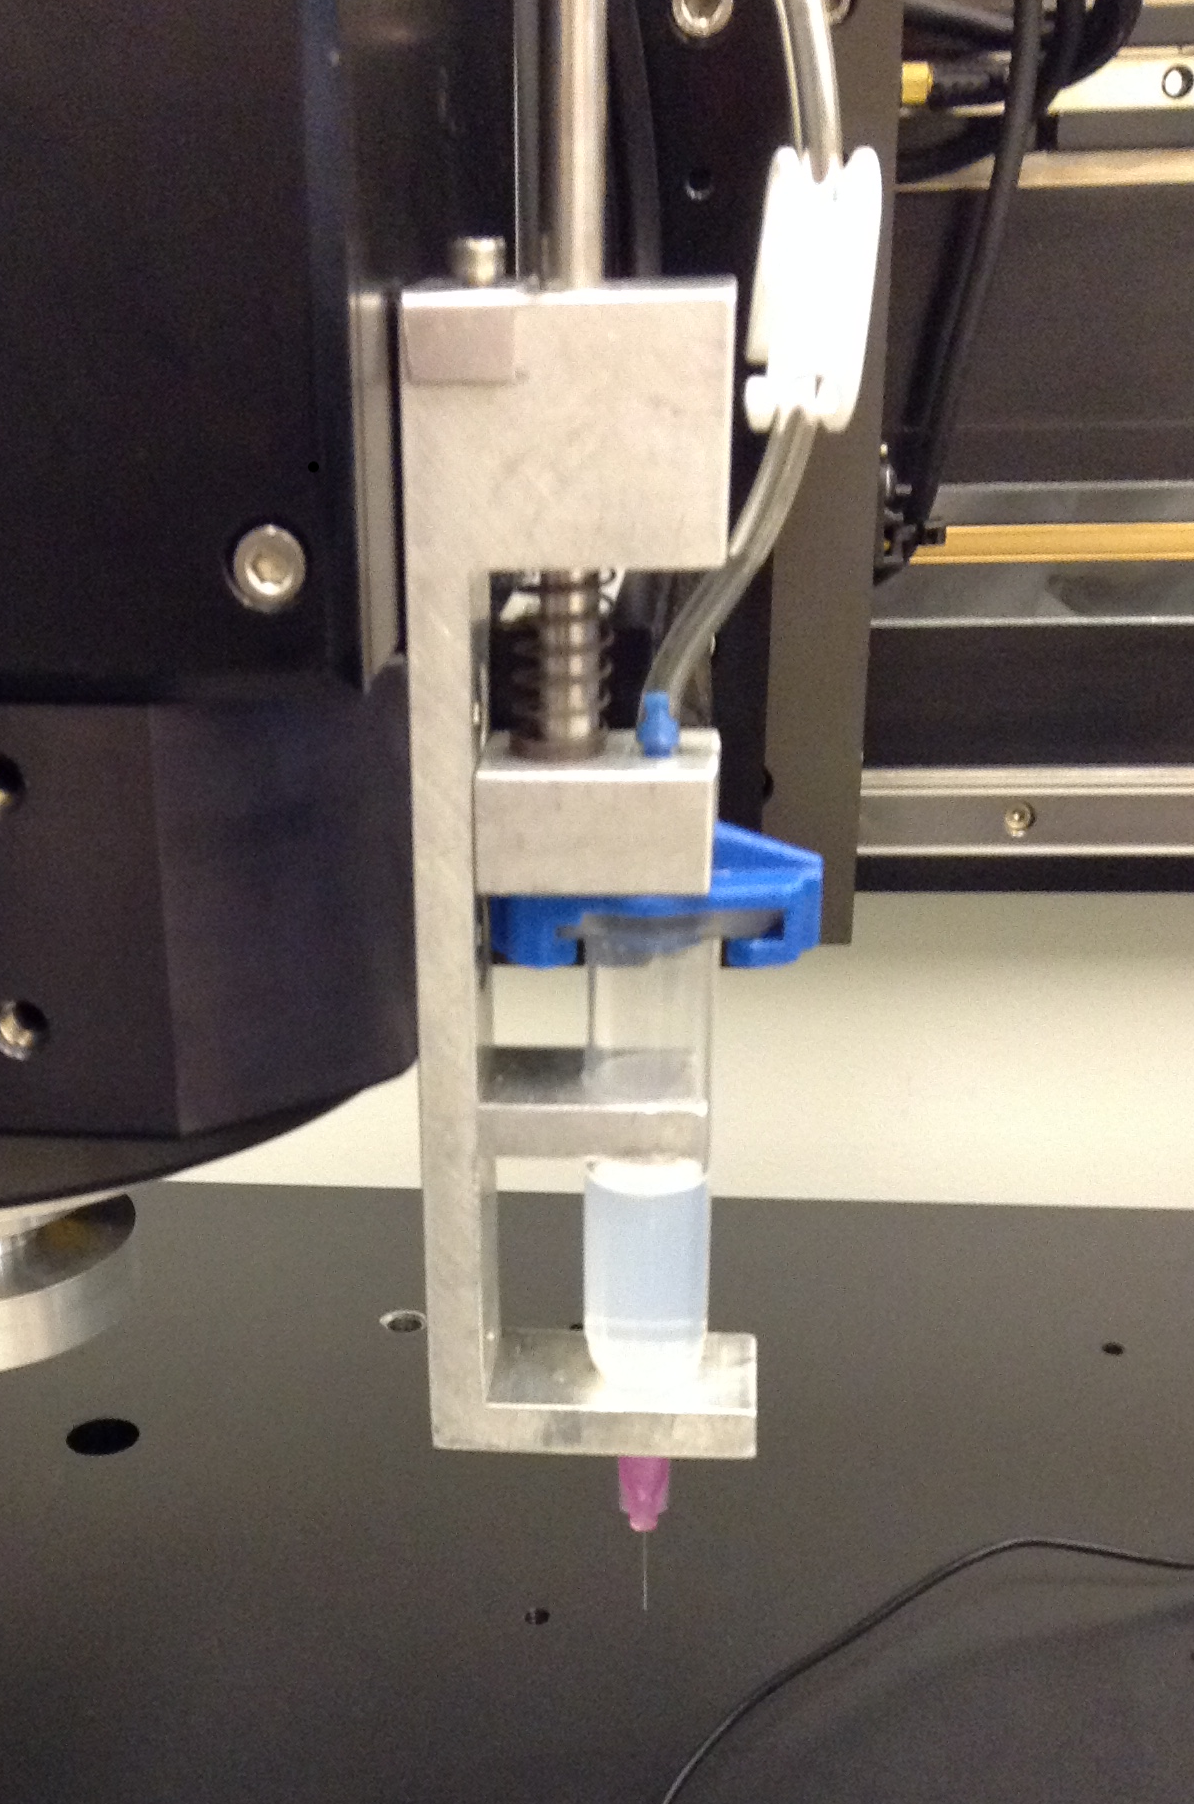
\includegraphics[width=0.45\textwidth,height=0.55\textwidth]{pixel/syringe.png}\\
    \includegraphics[width=0.45\textwidth,height=0.35\textwidth]{pixel/dispenser.png}
    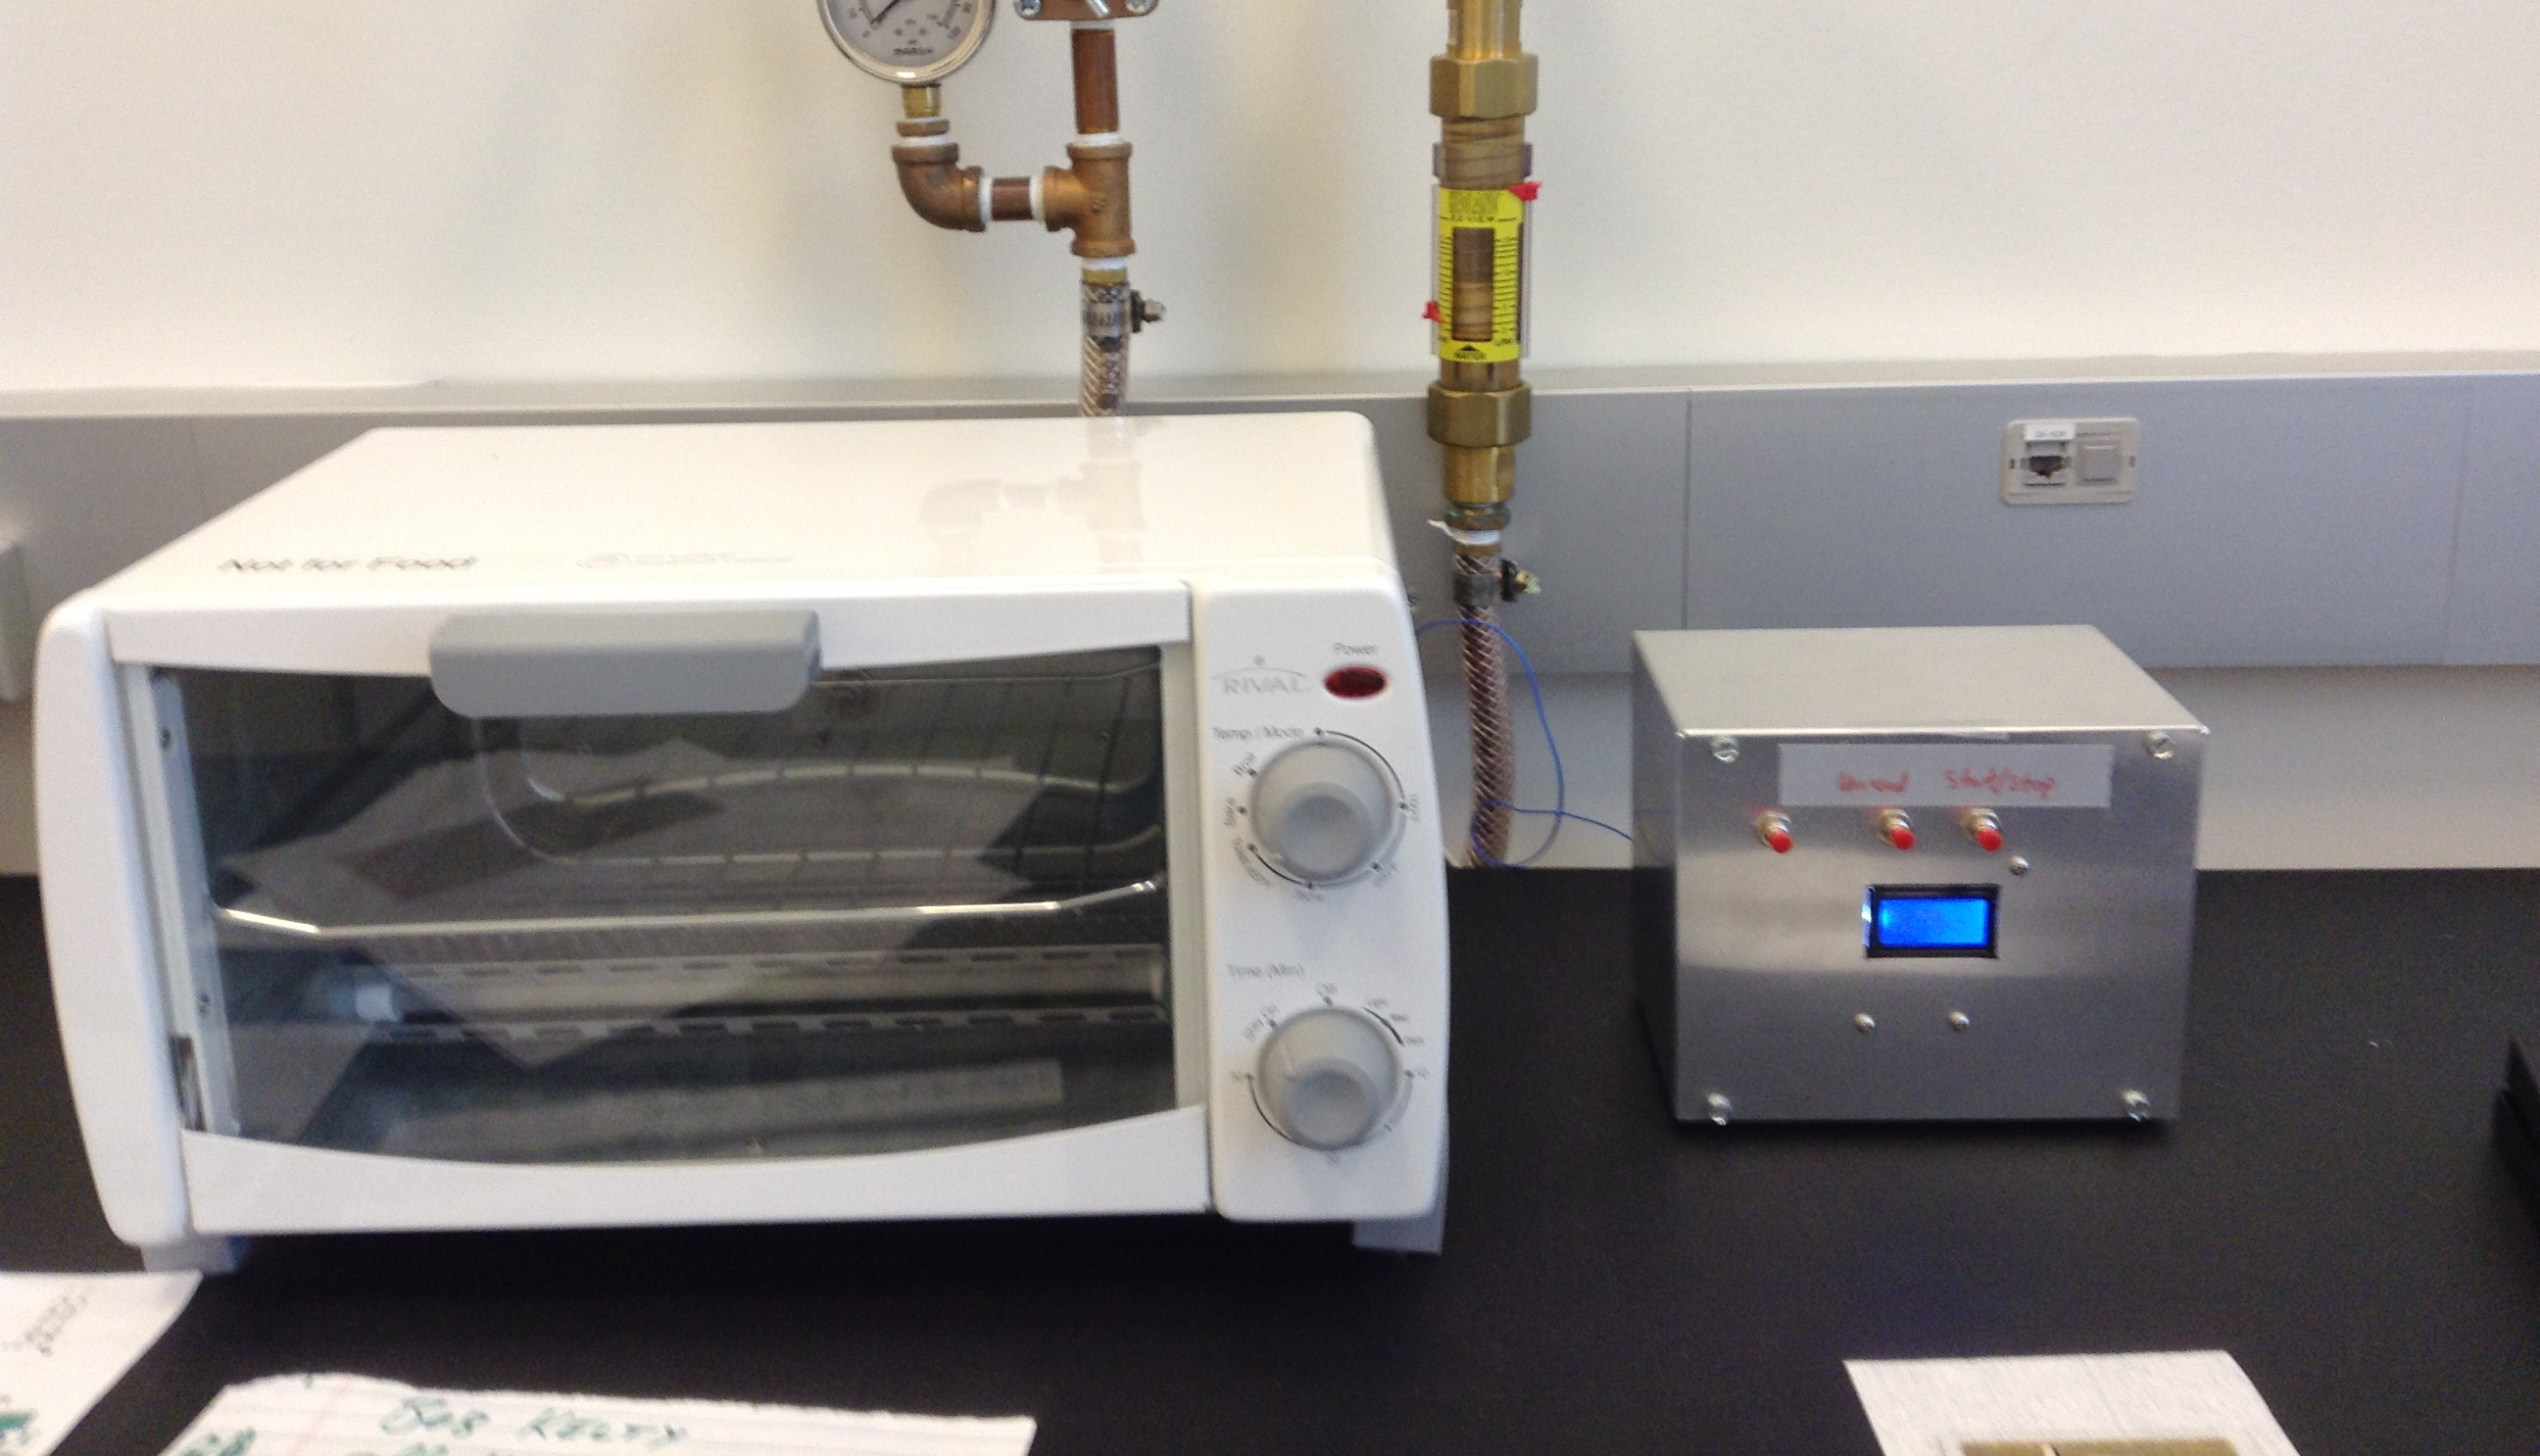
\includegraphics[width=0.45\textwidth,height=0.35\textwidth]{pixel/curing_oven.png}
    \caption[Dispensing system components.]{Dispensing system components.}\label{fig:potting_comp}
  \end{center}
\end{figure}

The encapsulation process consists of depositing a sylgard trace over the wires connecting the HDI and ths ROC; it is highly dependent not only on the ability to measure the location of the regions to be encapsulated, which is well managed by the vision system, but also on the ability to know with high precision the position of the needle tip, which added to the fact that for each encapsulation session a new set syringe-needle has to be used, demands a robust method to find the needle tip.

\begin{figure}[h]
  \begin{center}
    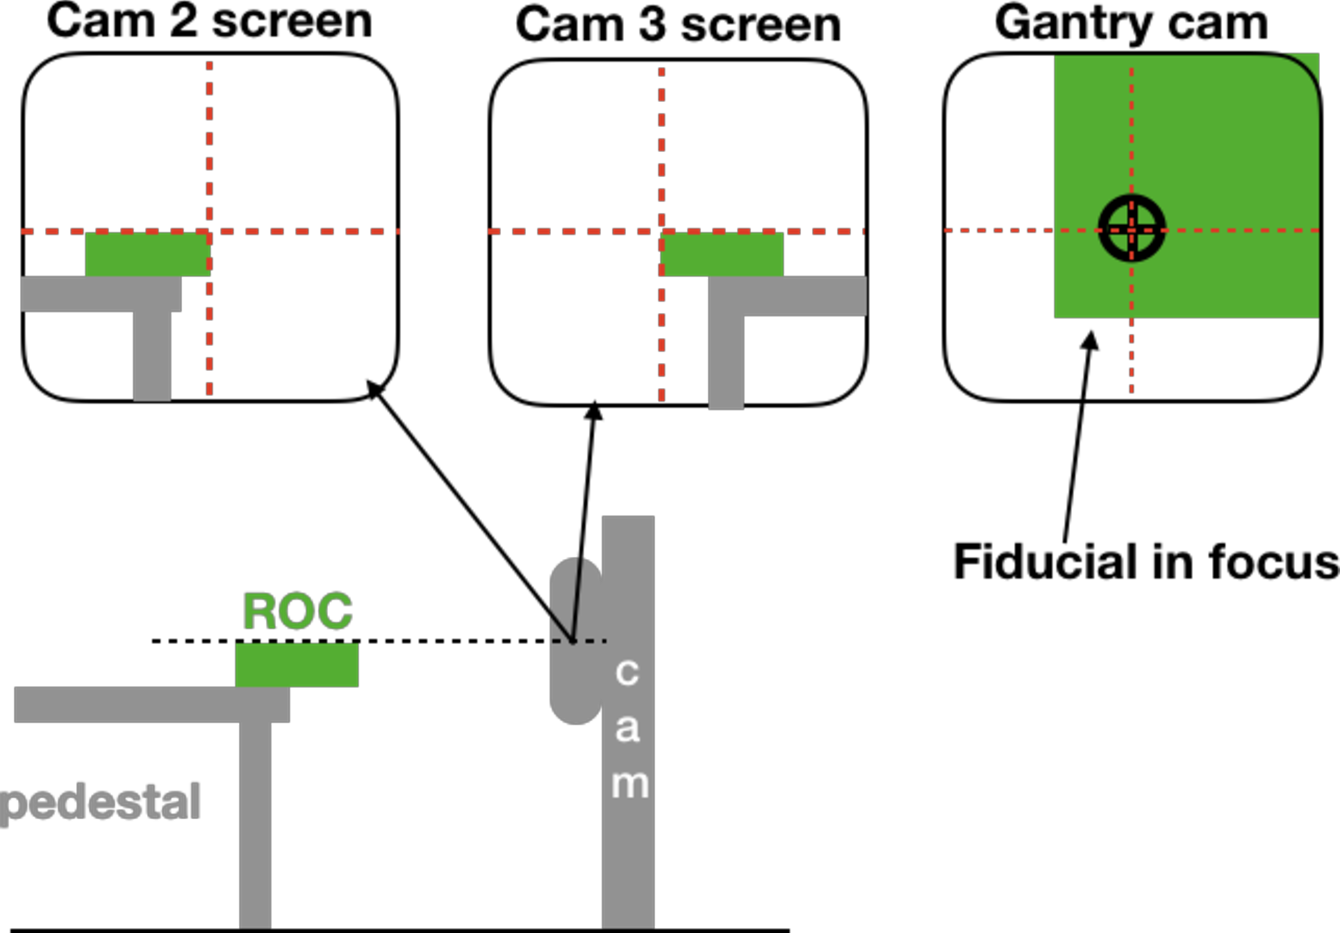
\includegraphics[width=0.55\textwidth,height=0.4\textwidth]{pixel/webcam_setup.png}
    \includegraphics[width=0.4\textwidth,height=0.5\textwidth]{pixel/webcam_setup2}
    %\includegraphics[width=0.45\textwidth,height=0.35\textwidth]{pixel/.png}
    %\includegraphics[width=0.45\textwidth,height=0.35\textwidth]{pixel/curing_oven.png}
    \caption[Webcam setup.]{Webcam setup used to locate the needle tip in 3D.}\label{fig:webcam_setup}
  \end{center}
\end{figure}

\begin{figure}[h]
  \begin{center}
    \includegraphics[width=0.40\textwidth,height=0.45\textwidth]{pixel/webcam_setup_cal2.pdf}
    \includegraphics[width=0.45\textwidth,height=0.45\textwidth]{pixel/webcam_setup_cal3.pdf}\\
    \caption[Webcam setup calibration.]{Webcam setup calibration. The 3D needle tip coordinates define the reference coordinates (origin) of the webcam setup.}\label{fig:webcam_cal}
  \end{center}
\end{figure}

The needle-tip calibration procedure was implemented using an additional vision system composed of two regular web cameras disposed one perpendicular to each other as shown in Figure \ref{fig:webcam_setup} known as \ti{webcam setup}. The reference position acting as the origin of the webcam setup coordinate system (RC) was defined by looking at a ROC placed over a pedestal so that the horizontal plane of the webcams is adjusted; then, using the gantry camera, a fiducial mark on the ROC was located and focused so that the $z$ coordinate of the fiducial is known ($RC_z$). Later, with a dispenser syringe and a needle tip mounted on the syringe holder, the needle tip was moved to the position of the fiducial mark on the ROC previously focused; the focuses of webcams were adjusted such that the needle is well visible in the screens (see Figure \ref{fig:webcam_cal}) and simultaneously in focus for both webcams, while the needle tip is centered in the screen, thus, ($x,y$) gantry head coordinates at that position correspond to the $(RC_x, RC_y)$ coordinates; after the calibration the RC is
\beqn 
  RC= (17.337,80.144, 88.486)\ mm
\eeqn

For any new needle to be used, it is necessary to correct for the needle tip coordinates deviation from the RC; the correction is obtained by moving the new needle tip to the RC position and adjusting the position of the needle tip to get it focused and centered in the webcam setup screens; these modified coordinates (MC) are compared with RC, and the difference is called \ti{Needle Tip Offset} (NTO); this calibration is connected to the calibration made for the GHCO so that the coordinates provided by the vision system for the regions to be encapsulated are also corrected for the NTO.              

\begin{figure}[h]
  \begin{center}
  \includegraphics[width=0.7\textwidth,height=0.3\textwidth]{pixel/nto}
  \caption[Needle tip offset measurement.]{Needle tip offset measurement.}\label{fig:webcam_adjust}
  \end{center}
\end{figure}

\subsubsection*{Space-time synchronization of the sylgard deposition}

The requirement imposed to the sylgard deposition over the modules, HDI and BBM, is to cover all the bond pads including the wire bonds; to do that, several parameters were optimized. First, when the sylgard starts to flow out of the needle, it is necessary that the sylgard drop gets in touch with a surface/object before it gets to heavy to fall down and prevent a continuous flow. Also, it is desired that the sylgard drop touches the HDI/BBM bondpads/surface first, rather than the wires themselves; in the former case, the sylgard spreads along the surface while in the latter case the sylgard sticks to the wires and it does not spread. Thus, the distance between the needle tip and the surface is a critical factor.

\begin{figure}[h]
  \begin{center}
    \includegraphics[width=0.7\textwidth]{pixel/bondpad_region}
    \caption[Wire bond region.]{Wire bond region.}\label{fig:bondpad_region}
  \end{center}
\end{figure}

Figure \ref{fig:bondpad_region} shows a schematic of the wire bond region and some typical dimensions involved. The slope of the wire is about $34^o$ but can vary according to the wirebonding conditions. Going too close to the surface would make the needle tip to touch and break the wires. If the reference to deposit the sylgard is chosen to be the center of the bond, \ie, the center of the needle will be right above the center of the bond, then a simple calculation of the height (h) necessary to have the wire at a safe distance from the needle tip is given by 

\beqn
h=\left(d+r_N-\frac{b}{2}\right )\tan(\theta)
\eeqn

\noindent where $d$ is the distance from the needle tip edge to the wire (safe distance), $r_N$ is the external needle radius ($310 \mu$m), $b$ is the size of the bond ($100 \mu$m) and $\theta$ describe the slope of the wire. Table \ref{tab:needle_tip_heights} shows the values of $h$ for several combinations of $d$ and $\theta$ ($r_N$ and $b$ fixed).
\begin{table}
  \centering
  \begin{tabular}{ c  c  c  c  c } \hline
               &\multicolumn{4}{c}{d($\mu$m)}\\\hline
  $\theta(^o)$ & 100   & 150   & 200   & 250 \\\hline
    30         & 207.8 & \textcolor{red}{236.7} & 265.6 & 294.4 \\
    45         & 360.0 & 410.0 & 460.0 & 510.0 \\
    60         & 623.5 & 710.1 & 796.7 & 883.3 \\\hline
  \end{tabular}
  \caption[Values of the needle tip height $h$]{Values of the needle tip height $h$ ($\mu$m) for several combinations of parameters $d$ and $\theta$. }\label{tab:needle_tip_heights}
\end{table}

Given the typical slope of the wires, it was chosen $h=236.7$ $\mu$m as the needle tip height.   

The next optimization was performed on the parameters defining the sylgard deposition kinematics. The basic sylgard deposition process consists of depositing a sylgard trace along a path defined by an initial and final positions $(x_i, y_i, z_i), (x_f, y_f, z_f)$. To make sure that all the wirebonds are covered, it is necessary to synchronize the dispenser action and the gantry motion. The top side of Figure \ref{fig:sylgard_synch} shows an sketch of the gantry speed and dispenser action as a function of the time. When the dispenser is open the sylgard starts to flow out of the needle, however, the sylgard needs some time to flow out and get touch the surface of the HDI/BBM, thus, there should be a time delay between the dispenser valve opening and the movement of the gantry, it is called $\Delta t_0$. Accordingly, after the valve is closed, there is a remaining sylgard flowing, so the valve should be  closed before the gantry reach the end of the way; this time delay is called $\Delta t_1$.

\begin{figure}[h]
  \begin{center}
    \includegraphics[width=0.75\textwidth]{pixel/time_delay}\\\ 
    \includegraphics[width=\textwidth]{pixel/space_delay}
    \caption[Sylgard deposition synchronization.]{Sylgard deposition synchronization. Top: sketch of the gantry velocity and dispenser action as a function of the time. Bottom: sketch of the strategy designed to determine the time delays.}\label{fig:sylgard_synch}
  \end{center}
\end{figure}

To find these time delays, the strategy sketched in the bottom side of Figure \ref{fig:sylgard_synch} was implemented in a LabVIEW program; it proceeds as follows: with the dispenser needle loaded and mounted on the syringe holder and the needle tip calibrated, a set of sylgard marks are deposited over a glass slide. The first is a control mark at $x_0$, then, at $x_1$ the gantry starts to move at constant speed $v$; at $x_2$ the dispenser valve is opened; at $x_3$ the sylgard gets in touch with the glass slide and it starts to spread. At $x_4$, the dispenser valve is closed, but some sylgard is still flowing out until $x_5$. At $x_6$, the gantry stops and finally, at $x_7$ another sylgard control mark is deposited. The time delays are given by 

\begin{align}
  \Delta t_0&=\frac{\Delta S_0}{v}=\frac{x_3-x_2}{v},\\
  \Delta t_1&=\frac{\Delta S_1}{v}=\frac{x_5-x_4}{v}
\end{align}

Figure \ref{fig:delays_measure} shows the results from two attempts to measure the time delays. In the first attempt, the samples were taken at intervals of five minutes at 1 mm/s; the sylgard traces started to break up after seven samples. The reason of the breaking up is that the sylgard gets ticker with time so that the speed of the gantry needs to be decreased. In the second attempt, the speed was decreased when the breaking up showed up; in total, forty samples spaced by five minutes were taken at six values of the speed (0.6,0.5,0.4,0.3,0.25) mm/s.

\begin{figure}[h]
  \begin{center}
    \includegraphics[width=0.48\textwidth,height=0.3\textwidth]{pixel/time_delays1.png} 
    \includegraphics[width=0.48\textwidth,height=0.3\textwidth]{pixel/time_delays2.png}
    \caption[Time delay measurements.]{Time delay measurement. Left: ten samples spaced by 5 minutes at 1mm/s. Right: forty samples spaced by 5 minutes, adjusting the speed to eliminate the breaking up..}\label{fig:delays_measure}
  \end{center}
\end{figure}

\begin{figure}[h]
  \begin{center}
    \includegraphics[width=0.7\textwidth,height=0.4\textwidth]{pixel/speed_function1.png}\\ 
    \includegraphics[width=0.8\textwidth]{pixel/time_delays3.png}
    \caption[Speed function for sylgard deposition.]{Top: speed evolution in time for the time delays determination. Bottom: time delays determination experiment after the implementation of the speed function. After 3.5 hours of data taking, there is no sign of sylgard breaking up.}\label{fig:speed_function}
  \end{center}
\end{figure}

Figure \ref{fig:speed_function} (top) shows the speed evolution as a function of time for the forty samples; the quadratic fit (modified) corresponds to a function that models a consistent reduction of the gantry speed in time such that the breaking up of the sylgard traces is avoided. This fitting function was implemented in the labVIEW program used to take the samples for the time delay calculation; the results are shown in the bottom side of Figure \ref{fig:speed_function} where it is clear that the implementation of the speed function meets the requirements. This speed function is called \ti{deposition speed}.

\begin{figure}[h]
  \begin{center}
    \includegraphics[width=0.45\textwidth]{pixel/dt0.png} 
    \includegraphics[width=0.45\textwidth]{pixel/dt1.png}
    \caption[Time delay functions.]{Time delay functions $\Delta t_0$ and $\Delta t_1$. In the time range of the typical encapsulation process, time delays are approximated by a constant; conservative values were adopted:  $\Delta t_0 =0.1$ s,  $\Delta t_1 = 1$ s.}\label{fig:time_delay_functions}
  \end{center}
\end{figure}

From this test it is also possible to extract the time delay functions (given that the deposition speed is a function of the time it is expected that the time delays also depends on time); they are shown in Figure \ref{fig:time_delay_functions}.

The typical encapsulation time per module is about five minutes, therefore, a full encapsulation session would last about one and a half hours in total, counting the time used to find the fiducial marks on the HDIs/BBMs and the regions where the sylgard will be deposited. In that time range, $\Delta t_0$ and $\Delta t_1$ could be approximated by a constant; a conservative choice was adopted: $\Delta t_0 =0.1$ s,  $\Delta t_1 = 1$ s.            

\subsection{The gluing routine}

\begin{figure}[h]
  \begin{center}
    \includegraphics[width=0.9\textwidth]{pixel/glue_workflow2}
    \caption[Gluing routine workflow.]{Gluing routine workflow.}\label{fig:glue_workflow}
  \end{center}
\end{figure}

A gluing session was defined as the process where four modules are assembled. The gluing routine workflow is shown in Figure\ref{fig:glue_workflow}; the green steps represent the steps that are performed more than once in the same session, while the red steps represent those performed by the operator. The routine was implemented in a LabVIEW program (\ti{Gluing\_main.vi}) that controls the sequence. The \ti{Main front panel} of the gluing routine, shown in Figure \ref{fig:gluing_front_main}, gathers the most relevant information about the gluing session, while each step in the routine has its dedicated front panel. The module gluing sequence begins by manually placing pre-tested, BBMs, HDIs and tools on their chucks. Figure \ref{fig:gluing_materials} shows the materials used during the gluing session; the aluminum squared tool is used to hold the gel-pack containing the BBMs while the vacuum pen is used to manipulate the BBMs.

\begin{figure}[h]
\begin{center}
  \includegraphics[width=0.58\textwidth, height=0.4\textwidth]{pixel/gluing_materials}
  \includegraphics[width=0.4\textwidth, height=0.4\textwidth]{pixel/gel_pack1}
 \caption[Materials used during gluing stage]{Materials used during gluing stage (left). BBMs on a Gel-pack.}\label{fig:gluing_materials}
\end{center}
\end{figure}

\begin{landscape}
\begin{figure}[h]
  \begin{center}
    \vspace{-2.5cm}
    \hspace{-1cm}
    \includegraphics[width=24cm,height=16cm]{pixel/gluing_front_main1.png}
    \caption[Gluing routine LabVIEW front panel]{Gluing routine LabVIEW front panel.}\label{fig:gluing_front_main}
    \vspace{-2cm}
    \hspace{-2cm}
  \end{center}
\end{figure}
\end{landscape}


Once the parts are in place, and the program is run, the BBM and HDI identification information (serial numbers) is collected\footnote{A batch numbering strategy was designed to identify the modules internally at UNL.} in the first step as well as the configuration of the gantry table, \ie, the BBM/HDI slots and tools to be used so that the vacuum system is properly activated. 

The camera is moved to view, recognize and find the fiducials locations on the BBMs, HDIs and tools. These locations are stored and shown in the Main and \ti{Find fiducials} front panels so that the operator can identify abnormal values from extreme misalignment and pattern recognition fails; that usually occurs when the plates are not properly placed on the chucks and/or when the fiducials do not appear in the camera field of view. In those cases, a manual fiducial finding option is available. The find fiducial front pannel is shown in Figure \ref{fig:find_fid_front} and a sample of the found fiducials on a HDI and a BBM is shown in Figure \ref{fig:fid_reco} indicating the located center of the fiducial with a green dot. After all the fiducials are identified, the operator has to check them and perform the necessary adjustments. Usually, the glue was prepared in parallel to the fiducial identification, reducing the session time.  

\begin{landscape}
\begin{figure}[h]
\begin{center}
    \vspace{-2.9cm}
    \hspace{-1cm}
    \includegraphics[width=24cm,height=16.5cm]{pixel/find_fid_front}
    \caption[Fiducial finder LabVIEW front panel]{Fiducial finder LabVIEW front panel.}\label{fig:find_fid_front}
    \vspace{-2cm}
    \hspace{-2cm}
\end{center}
\end{figure}
\end{landscape}


\begin{figure}[h]
\begin{center}
  \includegraphics[width=\textwidth]{pixel/fid_reco1}
 \caption[Fiducial finder step LabVIEW front panel]{Fiducial finder step LabVIEW front panel.}\label{fig:fid_reco}
\end{center}
\end{figure}

The glue application step starts by picking up the grabber tool from the tool rack, and grabbing the stamp tools from their chuck; after dipping the stamp tool in the glue reservoir, the epoxy is dispensed on the BBMs. The procedure is repeated as many times as the number of modules involved in the session, each time using a different stamp tool and a different glue reservoir slot. The step finishes by returning the grabber tool to the tool rack. The routine provides full freedom to choose any available combination of stamp tool, glue reservoir slot and BBM; this feature is particularly useful for glue testing and commissioning. The grabber tool is then returned to the tool rack and the picker tool is picked, so that the HDIs are picked from their plate slots and placed on top of the BBMs (making the alignment with respect to BBMs); again, the routine allows for different combinations of BBM-HDI. The front panels for both, gluing and pick-and-place steps, are shown in Figure \ref{fig:stamp_place_front}. Later, the picker tool is returned to the tool rack.

\begin{figure}[h]
\begin{center}
  \includegraphics[width=\textwidth]{pixel/stamp_front.png}
  \includegraphics[width=\textwidth]{pixel/place_front.png}
 \caption[Gluing and pick-and-place LabVIEW front panels]{Gluing (top) and pick-and-place (bottom) LabVIEW front panels.}\label{fig:stamp_place_front}
\end{center}
\end{figure}

In the weight step of the routine, the grabber tool is picked again from the tool rack in order to move the weight tools from their plate slots to the BBM locations. The front panel for this step is similar to the gluing front panel. Later, the grabber tool is returned to the tool rack and the gantry head is moved back to the home position. Figure \ref{fig:gluing_steps} shows pictures of the glue reservoir plate loaded with glue, BBMs after the glue deposition, BBM-HDI after pick-and-place, and weight tools over the assembled modules. 

\begin{figure}[h]
\begin{center}
  \includegraphics[width=0.4\textwidth,height=0.25\textwidth]{pixel/glue_reservoir_full.png}
  \includegraphics[width=0.4\textwidth,height=0.25\textwidth]{pixel/glue_on_bbm.png}\\
  \includegraphics[width=0.4\textwidth,height=0.25\textwidth]{pixel/bbm_hdi2.png}
  \includegraphics[width=0.4\textwidth,height=0.25\textwidth]{pixel/weight_on_bbm.png}
  \caption[Gluing steps pictures.]{Gluing steps pictures. Top: glue reservoir loaded (left), glue dispensed on BBMs (right). Bottom: BBM-HDI after pick-and-place(left), weight tools over assembled modules(right).}\label{fig:gluing_steps}
\end{center}
\end{figure}

The last step of the routine consists of creating and publishing the gluing session report (see Figure\ref{fig:gluing_report}) in the UNL silicon lab. electronic logbook (ELOG) and updating the database created to keep track of the assembly progress.  

\begin{figure}[h]
\begin{center}
  \includegraphics[width=\textwidth]{pixel/gluing_report}
 \caption[Gluing session report.]{Gluing session report.}\label{fig:gluing_report}
\end{center}
\end{figure}

At the end of the full cycle, the stamp plate with stamp tools is moved to be cleaned thoroughly using water and 2-propanol at sink outside the clean room; let them dry and bring them back to gantry table. The assembled modules are left to cure eight hours, typically overnight. The fully detailed SOP (SOP-103) for the gluing stage can be found in Reference \cite{sop_103}, while several videos showing the gluing routine in action can be found in References \cite{gluing_frank, jmonroy_channel}. 

\subsection{The encapsulation routine}

Following the assembly, HDIs are wirebonded to the ROCs using a semi-automated ultrasonic wirebonding machine. Pull tests of wirebonds are performed on a sample of modules for quality control; a picture of one of the sixteen ROCs wirebonded to its HDI counterpart is shown in Figure \ref{fig:wirebonds}. The wirebonds were encapsulated with an elastomeric compound in order to protect them from mechanical damage and to avoid possible shortcut circuits.

\begin{figure}[h]
\begin{center}
  \includegraphics[width=0.8\textwidth]{pixel/wirebond}
 \caption[ROC-HDI wirebonding.]{ROC-HDI wirebonding.}\label{fig:wirebonds}
\end{center}
\end{figure}

The encapsulation was performed using the robotic gantry and the dispensing system described in Section \ref{sec:setup}; the step by step instructions are documented in SOP-105 \cite{sop_105}. After the wirebonding, the plates with the modules were taken back to the gantry table and placed in the BBM chucks. The encapsulation strategy is based on a simple routine: by stating the initial conditions, \ie, the initial ($R_i$) and final ($R_f$) reference positions, the time elapsed after sylgard preparation, time delays, and needle tip location, the gantry head is moved to $R_i$ and the encapsulant is deposited following the structure sketched in Figure \ref{fig:sylgard_synch} (top). The sylgard trace is required to fully cover the HDI/BBM bond pads without spreading out in between the sensor and the ROC.

\begin{figure}[h]
\begin{center}
  \includegraphics[width=\textwidth]{pixel/potting_workflow}
  \caption[Encapsulation workflow.]{Encapsulation workflow. Steps in red correspond to interactions with the user; steps in blue are those performed by the gantry automatically while the step in green is performed by the gantry repeatedly during the same encapsulation session.}\label{fig:potting_workflow}
\end{center}
\end{figure}

An encapsulation session is defined as the process where 8 modules are encapsulated following the encapsulation routine workflow shown in Figure \ref{fig:potting_workflow}; steps in red correspond to actions performed by the user; steps in blue are those performed by the gantry automatically while the step in green is performed by the gantry repeatedly during the same encapsulation session. The routine was implemented in a LabVIEW program controlling the sequence, taking advantage of the routines created during the implementation of the gluing stage.   

The main routine is composed of two steps, although each step involves more than one substeps. Again, the most important information about the session is gathered in the main front panel as shown in Figure \ref{fig:potting_main_front}. The encapsulation routine involves much less vacuum manipulation given that there are no movable elements.

\begin{landscape}
\begin{figure}[h]
\begin{center}
    \vspace{-2.9cm}
    \hspace{-1cm}
    \includegraphics[width=24cm,height=16.5cm]{pixel/potting_main_front}
    \caption[Encapsulation LabVIEW main front panel]{Encapsulation LabVIEW main front panel.}\label{fig:potting_main_front}
    \vspace{-2cm}
    \hspace{-2cm}
\end{center}
\end{figure}
\end{landscape}

The module encapsulation sequence begins by moving the wirebonded modules from the storage cabinet to the chucks; since the session involves eight modules, only two chucks are made available in the routine. Once the module identification information and gantry table configuration are provided by the operator, the vacuum is activated accordingly.

In the first step, the vision system is used to locate the fiducial marks on the BBMs and HDIs, the same used in the gluing stage, and the reference positions that define the sylgard traces to be deposited. 

\begin{figure}[h]
\begin{center}
  \includegraphics[width=\textwidth]{pixel/hdi_bondpads}
 \caption[Encapsulation region.]{Encapsulation region. The sylgard trace, defined by the reference positions $R_i$ and $R_f$, is required spread out to fully cover the bond pads. }\label{fig:hdi_bondpads}
\end{center}
\end{figure}

These reference positions $R_i$ and $R_f$ define the length of the sylgard trace  as shown in Figure \ref{fig:hdi_bondpads}; they are determined from the bond pad locations which in turn are found using the information from the BBM/HDI design technical specifications, \ie, knowing the location of the fiducial marks on the BBM/HDI, it is possible to locate with precision the location of the bond pads. Originally, $R_i$ was identified with the center of the first bond pad, while $R_f$ was identified with the center of the last bond pad; however, the initial testing showed that this identification resulted in some of the pads not being fully covered. At first, the proposed solution was to extend $\Delta t_0$ and eliminate $\Delta t_i$ which would increase the amount of sylgard in the trace ends, but further testing showed that the additional amount of sylgard, due to an extended $\Delta t_0$, did not provide a full solution and that the surface tension would be source of the issue. A simple solution was to move the reference positions a bit away from the bond pad center as showed in Figure \ref{fig:hdi_bondpads}; this adjustment was implement in the routine. 

In general, the sylgard trace lives in 3D because the module is not perfectly aligned with respect to the gantry coordinate system (neither the HDI) and even thought the ROCs are flat the HDI could be bent, therefore, the gantry motion during the sylgard deposition is carried in 3D. The displacements in each direction are determined from the reference positions and the motions are done in the same time interval, thus, the speed for each direction is different; however, the displacement in $y$-direction, \ie, the length of the set of bond pads which is about 8 mm, is much larger than the displacement in $x$ and $z$ directions, which are expected to be about 10-50 $\mu$m, so essentially the speed in y-direction is essentially the same as the deposition speed.

The fact that the HDI is not perfectly flat, implies that even though the technical specifications can provide a very precise estimation of the references in the $x-y$ plane and at some extend the information from the fiducials locations can provide a measurement of the variation in $z$-direction, it is still necessary to set the reference positions independently for each sylgard trace in order to foreseen any bump in the HDI.

After the reference positions have been determined, they are approved by the operator or adjusted according to the parameters described above; in case of failure, a manual mode is available. Figure \ref{fig:potting_references} shows pictures with the reference positions chosen for a module.        

\begin{figure}[h]
\begin{center}
  \includegraphics[width=0.32\textwidth,height=0.32\textwidth]{pixel/pot_ref_hdi1.png}
  \includegraphics[width=0.32\textwidth,height=0.32\textwidth]{pixel/pot_ref_bbm2.png}
  \includegraphics[width=0.32\textwidth,height=0.32\textwidth]{pixel/pot_tbm1.png}
  \includegraphics[width=0.32\textwidth,height=0.32\textwidth]{pixel/pot_ref_hdi2.png}
  \includegraphics[width=0.32\textwidth,height=0.32\textwidth]{pixel/pot_ref_bbm1.png}
  \includegraphics[width=0.32\textwidth,height=0.32\textwidth]{pixel/pot_tbm2.png}
  \includegraphics[width=0.32\textwidth,height=0.32\textwidth]{pixel/pot_ref_add.png}
  \includegraphics[width=0.32\textwidth,height=0.32\textwidth]{pixel/pot_ref_hv_hdi.png}
  \includegraphics[width=0.32\textwidth,height=0.32\textwidth]{pixel/pot_ref_hv_bbm.png}
 \caption[Encapsulation reference positions.]{Encapsulation reference positions for one module. 1 and 4 show the reference positions for one of the HDI bond pads sets, while 2 and 5 show the corresponding reference positions for the bond pads on the BBM side. 3 and 6 show the reference points for the TBM; 7, 8 and 9 show the reference positions for the address pads, the HV pad on HDI and the HV pad on BBM respectively.}\label{fig:potting_references}
\end{center}
\end{figure}

The next step is the sylgard preparation; 1 cc of sylgard elastomer are mixed with 0.1 cc of curing agent over a plastic sheet and then transferred to the dispenser syringe using the spatula. Later, the dispenser syringe is placed in a clinical centrifuge in order to eliminate the air bubbles; finally the dispenser syringe is installed in the syringe holder attached to the gantry head. This process takes about ten minutes and is required to be done in the shortest time possible given that sylgard gets ticker with time; the mixing time has to be annotated and inputted into the program in order to control the deposition speed.

The needle tip is installed once the dispenser syringe is mounted in the holder, then, the needle tip calibration is performed using the webcam setup; before to start dispensing the sylgard, the syringe is purged to eliminate the air trapped between the syringe mouth and the needle tip.

In total, the encapsulation of one module is composed by 32 sylgard traces covering the bonds connecting the HDI and each of the 16 ROCs per module, 8 sylgard traces covering the bonds connection the TBM and the HDI, 2 sylgard traces covering the bonds of the address pads, and two sylgard drops covering the HV pads; each module is encapsulated in about five minutes. Figure \ref{fig:sylgard_dep} shows the sylgard deposition front panel. 

\begin{figure}[h]
\begin{center}
  \includegraphics[width=\textwidth]{pixel/sylgard_dep.png}
  \caption{Sylgard deposition LabVIEW front panel.}\label{fig:sylgard_dep}
\end{center}
\end{figure}

After the sylgard deposition step, the syringe is removed from the holder and the gantry head goes back to home position. The work at the gantry table ends with the generation and publication of the encapsulation session report (see Figure \ref{fig:potting_report}).   

\begin{figure}[h]
\begin{center}
  \includegraphics[width=\textwidth]{pixel/potting_report}
 \caption[Encapsulation session report.]{Encapsulation session report.}\label{fig:potting_report}
\end{center}
\end{figure}

At the end of the full cycle, a visual inspection of the sylgard traces is performed in order to ensure the quality of the encapsulation; in case of defects, the encapsulation procedure is repeated taking the reference positions in agreement with the regions that are not fully sylgard-covered. Several videos showing the encapsulation routine in action can be found in Reference\cite{jmonroy_channel}.

\begin{figure}[h]
\begin{center}
  \includegraphics[width=0.32\textwidth,height=0.42\textwidth]{pixel/potting_test.png}
  \includegraphics[width=0.32\textwidth,height=0.42\textwidth]{pixel/ROC_HDI_bonds1.png}
  \includegraphics[width=0.32\textwidth,height=0.42\textwidth]{pixel/pot_res_tbm.png}
  \includegraphics[width=0.45\textwidth,height=0.32\textwidth]{pixel/pot_res_add.png}
  \includegraphics[width=0.45\textwidth,height=0.32\textwidth]{pixel/pot_res_hv.png}
  \caption[Encapsulation results.]{Encapsulation results. 1 shows an encapsulation test. 2-5 show the results from a module encapsulation for two sets of ROC-HDI traces, TBM, address pads and HV pads respectively.}\label{fig:potted_module}
\end{center}
\end{figure}

Later, the plates with the encapsulated modules are transferred into the curing oven where they are submitted to a thermal cycle keeping them at 50 $^o$C degrees for one hour. The curing procedure is not included in the encapsulation routine and no details are provided about it in this document. Figure \ref{fig:potted_module} shows a picture of an encapsulation test using a plain HDI glued on a glass slide; also, pictures of an encapsulated module confirming the quality of the encapsulation.  

The module assembly sites were also responsible for the testing and characterization of the assembled pixel modules; therefore, modules were tested at room temperature ($\sim$ 17 $^o$C) while monitoring ROC
digital and analog currents. The very last step in the production line was the shipment to the $X-rays$ characterization site located at the University of Kansas. Figure \ref{fig:module_in_carrier} shows a module in the carrier ready to be shipped; a plastic lid, not showed, was used to fully cover the module.       

\begin{figure}[h]
\begin{center}
  \includegraphics[width=0.8\textwidth]{pixel/module_in_carrier}
 \caption[Module in carrier.]{Module in carrier. A plastic lid was used to fully cover the module.}\label{fig:module_in_carrier}
\end{center}
\end{figure}

\subsection{FPix module production yields}

Figure \ref{fig:mod_ass_time} shows the module assembly over time for both assembly sites and for UNL; in total 1224 were assembled, 555 of them at UNL. At the integration site (SiDet-Fermilab), modules were submitted to testing in order to ensure they are fully functional and fulfill the performance requirements; a detailed description of the complete set of tests is documented in Reference \cite{fpix_module_testing_guide}.

\begin{figure}[h]
\begin{center}
  \includegraphics[width=0.8\textwidth]{pixel/mod_ass_time}
  \includegraphics[width=0.8\textwidth]{pixel/mod_ass_unl}
 \caption[Module assembly over time.]{Module assembly over time for both assembly sites(top) and for UNL (bottom).}\label{fig:mod_ass_time}
\end{center}
\end{figure}

After testing, each module is given a grade based on its IV performance and its single pixel defects as stated in Table \ref{tab:grad_scheme}. The IV performance refers to two aspects; on one side, the amount of leakage current at the expected operating bias voltage ($I_{-150\textrm{V}}$), and on other side, to the breakdown voltage which should be higher than -150 V. If the breakdown voltage is lower than -150 V, the ratio $I_{-150V}/I_{-100V}$ should be small, otherwise it should be large.      

\begin{table}
  \centering
  \begin{tabular}{ c  c  c  c  c } \hline
                                    &                       & \multicolumn{3}{c}{Grade} \\\hline
                                    & Criteria              & A        &  B         &   C       \\\hline
    \multirow{2}{*}{IV performance} & $I_{-150V}$           & $<2\mu$A &  $<10\mu$A & $>10\mu$A \\
                                    & $I_{-150V}/I_{-100V}$ & $<2$     &  $<2$      & $>2$      \\\hline
    Pixel defects                   & Sum per ROC           & $<1$\%   &  $<4$\%    & $>4$\%    \\\hline
  \end{tabular}
  \caption[FPix module grading scheme.]{FPix module grading scheme. The overall module grade is assigned as the worse of the IV grade and the pixel defect grade.}\label{tab:grad_scheme}
\end{table}

\begin{figure}[h]
\begin{center}
  \includegraphics[width=0.6\textwidth]{pixel/mod_grade_time}
  \includegraphics[width=0.8\textwidth]{pixel/mod_grade_batch}
  \caption[Module grade over time.]{Module grade over time (top) and per received batch at the integration site(bottom).}\label{fig:mod_grad_time}
\end{center}
\end{figure}
Figure \ref{fig:mod_grad_time} shows the module grading yields over time as well as the module grading yields by batch received at the integration site; while in the first weeks of modules production the modules were mainly C-graded, due to a combination of failures in the quality of the HDIs and BBM received at the assembly sites and technical issues involving the production line, the quality of the modules was improved and about 620 A-graded modules were produced in the whole production time. At the integration time, not enough A-graded modules were available, therefore, B-graded modules were used to complete the 672 modules installed in the FPix detector; B-grade modules were installed in the outermost rings. C-graded modules were not used. Figure \ref{fig:fpix_mounted} shows the FPix installed in the CMS detector.

\begin{figure}[h]
\begin{center}
  \includegraphics[width=\textwidth]{pixel/fpix_mounted}
  \caption{FPix installed in the CMS detector.}\label{fig:fpix_mounted}
\end{center}
\end{figure}

